\documentclass[lablogo]{thesis}


\title{Secure Interface Design \\Leveraging Hardware/Software Support}
\author{Atri Bhattacharyya}
\president{Prof. Carmela González Troncoso}
\director{Prof. Mathias Payer}
\codirector{Prof. Babak Falsafi}
\internal{Prof. Sanidhya Kashyap}
\external{Dr. Anil Kurmus, IBM Research}
\external{Dr. Anjo Lucas Vahldiek-oberwagner, Intel Labs}

\cv{resume/main.pdf}

%%%%%%%%%%%%%%%%%%%%%%%%%%%%%%%%%%%%%%%%%%%%%%%%%%%%%%%%%%%%%%%%%%%%%
%%%%%%%%%%%%%%%%%%%%%%%%%%%%%%%%%%%%%%%%%%%%%%%%%%%%%%%%%%%%%%%%%%%%%
%%%%%%%%%%%%% Standard list of used packages %%%%%%%%%%%%%%%%
%%%%%%%%%%%%%%%%%%%%%%%%%%%%%%%%%%%%%%%%%%%%%%%%%%%%%%%%%%%%%%%%%%%%%
% \usepackage{cite}
\usepackage{amsmath,amsfonts}
% \usepackage{amssymb, amsfonts}
\usepackage{graphicx}
\usepackage{textcomp}
\usepackage{xcolor}
\usepackage{fancyhdr}
\usepackage{booktabs}
% \usepackage[hyphens]{url}
\usepackage[mathscr]{euscript}

% \usepackage[normalem]{ulem}

% Atri's list of typically used packages
% List of unused packages from Midas/TikTok
\usepackage{adjustbox}
% \usepackage{amsmath}
% \usepackage{filecontents}
% \usepackage{tikz}
\usepackage{xspace}
\usepackage{listings}
% \usepackage{xcolor}
% \usepackage{textcomp}
% \usepackage{graphicx}
% \usepackage{caption}
% \usepackage{subcaption}
% \usepackage{todonotes}
\usepackage{multirow}
\usepackage{multicol}
% \usepackage{booktabs}
\usepackage{paralist}       % For inparaenum
% \usepackage{enumitem}
% \usepackage{tabulary}
% \usepackage{verbatim}
\usepackage{balance}
\usepackage{tabularx}
\usepackage{algorithm}
\usepackage{algpseudocode}
\usepackage{braket}         % Fancy brackets
\usepackage{threeparttable} % Table with footnotes
\usepackage{makecell}       % Fancy multiline cells in table
\usepackage{pifont}         % For fancy dingbats, example xmark
\usepackage{comment}        % For comment environment
\usepackage{prettyref}    % For labels for autoref
% \usepackage[bookmarks=true,breaklinks=true,letterpaper=true,colorlinks,linkcolor=black,citecolor=blue,urlcolor=black]{hyperref}
                            % For autoref
\usepackage{listofitems}    % For `readlist` used for \newreviewer command
\usepackage{soul}           % For strikethrough \st
\usepackage{array}          % For whole row `\rowstyle'


%%%%%%%%%% Sid's list of packages %%%%%%%%%%
% \usepackage[normalem]{ulem}
% \usepackage[final]{microtype}
% \usepackage[keeplastbox]{flushend}
% \usepackage{soul}
% \usepackage{makecell}
% \usepackage{hyphenat}
% \usepackage{subfig}
% \usepackage{color}
% \usepackage{balance}    
% \usepackage{verbatimbox}
% \usepackage{fancyvrb}
% \usepackage{enumitem}

%%%%%%%%%% Packages borrowed from Ahmad's thesis %%%%%%%%%%%%%%%%%%
% \usepackage{titlesec}
% \titleformat{\chapter}[display]
%   {\normalfont\huge\bfseries}{\chaptertitlename\ \thechapter}{20pt}{\Huge}
% \titlespacing*{\chapter}{0pt}{-20pt}{40pt}

% \usepackage{xcolor}
% \usepackage{xspace}
\usepackage{epigraph}
% \usepackage{enumitem}                 % custom lists
% \usepackage{listings}                 % code formatting
% \usepackage{tikz}
% \usepackage{expl3}
% \usepackage{caption}                  % figure captioning
% \usepackage{subcaption}               % subfigures
% \usepackage{listofitems}              % \readlist
% \usepackage{fontawesome}              % faArrowUp, etc...
% \usepackage{siunitx}                  % \num, SI units
% \usepackage{xpatch}                   % \xapptocmd
% \usepackage{minted}                   % listing environment (TODO replace with consistent code listings)
% \usepackage{algorithm}                % algorithm environment
% \usepackage{algpseudocode}            % \algnewcommand, \Procedure, \Call, etc...
% \usepackage{varwidth}                 % varwidth environment
% \usepackage{fmtcount}                 % \numberstringnum
% \usepackage{refcount}                 % \getrefnumber
% \usepackage{soul}                     % \sethlcolor
% \usepackage{adjustbox}                % adjustbox environment
% \usepackage{booktabs}                 % \toprule
% \usepackage{multirow}                 % \multirow
% \usepackage{colortbl}                 % \cellcolor
% \usepackage{pifont}                   % \ding
% \usepackage{makecell}                 % \multirowcell
% \usepackage{rotating}                 % sideways environment
% \usepackage{pgfplots}                 % axis environment
% \usepackage{csquotes}                 % \enquote
% % \usepackage{annotate-equations}
% \usepackage{bbding}                   % \XSolidBold
% \usepackage{ifsym}                    % \textifsymbol
% \usepackage{nicefrac}                 % \nicefrac
% % \usepackage{amsmath}
% \usepackage{amssymb}                  % \npreceq etc...
% \usepackage{pgf-umlsd}                % sequencediagram environment
% \usepackage{tikz-layers}
% \usepackage{scalerel}
% \usepackage{graphicx}
% \usepackage{threeparttable} % Table with footnotes
% \usepackage[
%   backend=bibtex,
%   style=numeric-comp,
%   hyperref=true,
%   defernumbers=true,
%   maxbibnames=99,
%   maxcitenames=1
% ]{biblatex}
% \addbibresource{thesis.bib}

%%%%%%%%%%%%%%%%%%%%% Commenter's sections %%%%%%%%%%%%%%%%%%%%%%%
% Enable or disable reviews
\newif\ifreview
\reviewtrue   % comment this line to disable reviews
% newreviewer command description
\newcounter{ReviewerID}
\readlist*\annotationcolors{blue, red, orange, green, purple, yellow, brown, olive}
\newcommand{\newreviewer}[2]{%
  \ifnum \theReviewerID=\annotationcolorslen
    \setcounter{ReviewerID}{0} % cycle through colors
  \fi
  \stepcounter{ReviewerID}%
  \expandafter\edef\csname bootstrap#1\endcsname{%
    \expandafter\def\csname #1\endcsname####1{%
      \ifreview%
        {\noexpand\color{\annotationcolors[\theReviewerID]} {\noexpand\bf{\noexpand\fbox{#2}} {\noexpand\it ####1} }}
      \else%
        {}% disable annotations
      \fi%
    }%
  }%
  \csname bootstrap#1\endcsname%
}
% List of reviewers
% Command: \newreviewer{latexcommand}{visiblename}
% You will be able to use a command \latexcommand{comment}
% to generate a colored comment prepended by visiblename.
\newreviewer{mat}{Mat}
\newreviewer{atri}{AB}
% \newreviewer{florian}{FH}
\newreviewer{babak}{BF}
% \newreviewer{andres}{AS}
% \newreviewer{yuanlong}{YL}
% \newreviewer{sg}{Sid}
% \newreviewer{ant}{AV}
% \newreviewer{ahmad}{AH}
% \newreviewer{nicolas}{NB}

\graphicspath{{./media}}

\makeatletter
\providecommand*{\input@path}{}
\g@addto@macro\input@path{{./chapters/}} % append
\makeatother

%%%%%%%%%%%%%%%%%%%%%%%%%%%%%%%%%%%%%%%%%%%%%%%%%%%%%%%%%%%%%%%%%%%%%
%%%%%%%%%%%%%%%%%%%%%%%%%%%%%%%%%%%%%%%%%%%%%%%%%%%%%%%%%%%%%%%%%%%%%
% SecureCells definitions
%%%%%%%%%%%%%%%%%%%%%%%%%%%%%%%%%%%%%%%%%%%%%%%%%%%%%%%%%%%%%%%%%%%%%
\newcommand{\seccells}{SecureCells\xspace}
\newcommand{\ptable}{PTable\xspace}
\newcommand{\gtable}{GTable\xspace}
\newcommand{\cell}{cell\xspace}
\newcommand{\cellx}  [1]{$Cell_{#1}$\xspace}
\newcommand{\secdiv}{SD\xspace}
\newcommand{\secdivx}[1]{$SD_{#1}$\xspace}
% List of SD/SC instructions
\newcommand{\sdswitch}{\Code{SDSwitch}\xspace}
\newcommand{\sdentry} {\Code{SDEntry}\xspace}
\newcommand{\scprot}  {\Code{SCProt}\xspace}
\newcommand{\scgrant} {\Code{SCGrant}\xspace}
\newcommand{\screcv}  {\Code{SCRecv}\xspace}
\newcommand{\sctfer}  {\Code{SCTfer}\xspace}
\newcommand{\scinval} {\Code{SCInval}\xspace}
\newcommand{\screval} {\Code{SCReval}\xspace}
\newcommand{\scexcl}  {\Code{SCExcl}\xspace}
% List of SD/SC registers
\newcommand{\sid}{$SDID$\xspace}
\newcommand{\rid}{$RID$\xspace}
\newcommand{\xid}{\Code{XID}\xspace}
% Requirements
\newcommand{\req}[1]{\textbf{O#1}\xspace}

%%%%%%%%%%%%%%%%%%%%%%%%%%% Atri's design choices %%%%%%%%%%%%%%%%%%%%%%%%%%%%

\newenvironment{minilisting}
  {\minipage[b]{\linewidth}\verbatim}
  {\endverbatim\endminipage}

\lstdefinestyle{cstyle}{
  basicstyle=\footnotesize\ttfamily,
  keywordstyle=\color{black!85}\bfseries,
  keywordstyle=[2]\color{black!85}\bfseries\emph,
  showstringspaces=false,
  language={C},
  breaklines=false,
  mathescape=true,
  escapechar={@}
}
\lstdefinestyle{inline}{
  style=cstyle,
  mathescape=false,
  breaklines=true,
  keywordstyle=,
  keywordstyle=[2],
  extendedchars=true,
  basicstyle=\ttfamily\small
}
\newcommand{\Code}[1]{\lstinline[style=inline,breaklines=false]@#1@}
\let\realparagraph\paragraph
\let\paragraph\relax
\newcommand{\paragraph}[1]{\textbf{#1.}}
% \newcolumntype{Q}{>{\centering\arraybackslash}X}
% \newcolumntype{M}[1]{>{\centering\arraybackslash}m{#1}}

% These old were useful with the prettyref package
% Now overruled by the autoref package
% \newrefformat{cha}{\hyperref[#1]{Chapter~\ref*{#1}}}
% \newrefformat{sec}{\hyperref[#1]{Section~\ref*{#1}}}
% \newrefformat{sub}{\hyperref[#1]{Section~\ref*{#1}}}
% \newrefformat{tab}{\hyperref[#1]{Table~\ref*{#1}}}
% \newrefformat{fig}{\hyperref[#1]{Figure~\ref*{#1}}}
% \newrefformat{line}{\hyperref[#1]{line~\ref*{#1}}}
% \newrefformat{lst}{\hyperref[#1]{Listing~\ref*{#1}}}
% \newrefformat{pat}{\hyperref[#1]{Patch~\ref*{#1}}}
% \newrefformat{alg}{\hyperref[#1]{Algorithm~\ref*{#1}}}
% Customizing reference formats for
\addto\extrasenglish{%
\renewcommand{\sectionautorefname}{Section}
\let\subsectionautorefname\sectionautorefname
\let\subsubsectionautorefname\sectionautorefname
\renewcommand{\chapterautorefname}{Chapter}
}


\newcommand{\algorithmautorefname}{Instruction}
% Custom naming for algorithm, used for table of securecells instructions
\makeatletter
\newcommand{\removelatexerror}{\let\@latex@error\@gobble}
\renewcommand{\ALG@name}{Instruction}
\makeatother

% Custom command for making formatting changes to an entire row in tables
% For example, \setrow{\bfseries} in front of a row to make it bold
% https://tex.stackexchange.com/questions/4811/make-first-row-of-table-all-bold
\newcolumntype{!}{>{\global\let\currentrowstyle\relax}}
\newcolumntype{?}{>{\currentrowstyle}}
\newcommand{\rowstyle}[1]{\gdef\currentrowstyle{#1}%
  #1\ignorespaces
}

% Cross and tick marks
\newcommand{\cmark}{\ding{51}}%
\newcommand{\xmark}{\ding{55}}%

% Aliases:
% yes: for checkmark to make readable
\newcommand{\yes}{\checkmark}

% End of SecureCells definitions
%%%%%%%%%%%%%%%%%%%%%%%%%%%%%%%%%%%%%%%%%%%%%%%%%%%%%%%%%%%%%%%%%%%%%

%%%%%%%%%%%%%%%%%%%%%%%%%%%%%%%%%%%%%%%%%%%%%%%%%%%%%%%%%%%%%%%%%%%%%
%%%%%%%%%%%%%%%%%%%%%%%%%%%%%%%%%%%%%%%%%%%%%%%%%%%%%%%%%%%%%%%%%%%%%
% Midas definitions
%%%%%%%%%%%%%%%%%%%%%%%%%%%%%%%%%%%%%%%%%%%%%%%%%%%%%%%%%%%%%%%%%%%%%

%%%%% Duplicate from SecureCells, commented out
% \newenvironment{minilisting}
% {\minipage[b]{\linewidth}\verbatim}
% {\endverbatim\endminipage}

% \lstdefinestyle{cstyle}{
% basicstyle=\footnotesize\ttfamily,
% keywordstyle=\color{black!85}\bfseries,
% keywordstyle=[2]\color{black!85}\bfseries\emph,
% showstringspaces=false,
% language={C},
% breaklines=false,
% mathescape=true,
% escapechar={@}
% }
% \lstdefinestyle{inline}{
% style=cstyle,
% mathescape=false,
% breaklines=true,
% keywordstyle=,
% keywordstyle=[2],
% extendedchars=true,
% basicstyle=\ttfamily\small
% }
% \newcommand{\Code}[1]{\lstinline[style=inline,breaklines=false]@#1@}
% \let\realparagraph\paragraph
% \let\paragraph\relax
% \newcommand{\paragraph}[1]{\textbf{#1.}}
% \newcolumntype{Q}{>{\centering\arraybackslash}X}
% \newcolumntype{M}[1]{>{\centering\arraybackslash}m{#1}}

\newcommand{\tocttou}{TOCTTOU\xspace}
\newcommand{\midas}{Midas\xspace}

%%% More repitition from SecureCells
%   \newrefformat{cha}{\hyperref[#1]{Chapter~\ref*{#1}}}
%   \newrefformat{sec}{\hyperref[#1]{Section~\ref*{#1}}}
%   \newrefformat{sub}{\hyperref[#1]{Section~\ref*{#1}}}
%   \newrefformat{tab}{\hyperref[#1]{Table~\ref*{#1}}}
%   \newrefformat{fig}{\hyperref[#1]{Figure~\ref*{#1}}}
%   \newrefformat{line}{\hyperref[#1]{line~\ref*{#1}}}
%   \newrefformat{lst}{\hyperref[#1]{Listing~\ref*{#1}}}
%   \newrefformat{pat}{\hyperref[#1]{Patch~\ref*{#1}}}
%   \newrefformat{alg}{\hyperref[#1]{Algorithm~\ref*{#1}}}
%   \renewcommand{\sectionautorefname}{Section}
%   \let\subsectionautorefname\sectionautorefname
%   \let\subsubsectionautorefname\sectionautorefname

\renewcommand\itemautorefname{Attack}

% Probably don't need DOI for artificat
\newcommand{\doinumber}{5753026}
\newcommand{\zenodorecord}[0]{\url{https://zenodo.org/record/\doinumber}}
\newcommand{\zenododoi}[0]{10.5281/zenodo.\doinumber\xspace}

\newcommand{\footremember}[2]{%
   \footnote{#2}
    \newcounter{#1}
    \setcounter{#1}{\value{footnote}}%
}
\newcommand{\footrecall}[1]{%
    \footnotemark[\value{#1}]%
}

% End of Midas definitions
%%%%%%%%%%%%%%%%%%%%%%%%%%%%%%%%%%%%%%%%%%%%%%%%%%%%%%%%%%%%%%%%%%%%%


%%%%%%%%%%%%%%%%%%%%%%%%%%%%%%%%%%%%%%%%%%%%%%%%%%%%%%%%%%%%%%%%%%%%%
%%%%%%%%%%%%%%%%%%%%%%%%%%%%%%%%%%%%%%%%%%%%%%%%%%%%%%%%%%%%%%%%%%%%%
% Thesis front matter
%%%%%%%%%%%%%%%%%%%%%%%%%%%%%%%%%%%%%%%%%%%%%%%%%%%%%%%%%%%%%%%%%%%%%

% Change epigraph length to fix Adams' quote
\setlength\epigraphwidth{.45\textwidth}

\begin{dedication}
  \epigraph{
    \raggedleft
    Let us think the unthinkable, \\
    Let us do the undoable, \\
    Let us prepare to grapple with the ineffable itself, \\
    And see if we may not eff it after all.
  }{\textit{Douglas Adams}}
  \begin{absolute}
    \makebox[0pt]{\parbox{\textwidth}{
      \centering
      TODO: To the lack of humanity
    }}
  \end{absolute}
\end{dedication}

\begin{acknowledgments}
"
It's a dangerous business, Frodo, going out your door. 
You step onto the road, and if you don't keep your feet, there's no knowing where you might be swept off to.
”, 
Bilbo Baggins often said to his young nephew Frodo Baggins. 
When I left India to start a Masters program at EPFL in 2016,
little did I know of the journey that lay ahead. 
Looking back at the path culminating in the attainment of the doctorate, 
I must thank the many people who accompanied me through my wanderings, 
sweeping me off on unknown paths
and bringing light  in times of darkness.

Every journey requires guidance, and first I would like to thank my academic advisors,
Prof. Mathias Payer and Prof. Babak Falsafi, who led me through my PhD.
Mathias has been a source of constant inspiration throughout the years,
with his belief that all systems are definitely and undeniably ``broken''.
Mathias has been critical to my successes during the PhD, pushing me to try
every new avenue, teaching me to believe in my ideas, and providing the ever present
support required to make ideas real. 
My thesis is the culmination of a long series of ideas and ``weekend projects'' of 
increasing depth and clarity.
Many of the ideas comprising this thesis are the result of ideas refined and
polished into clarity with Mathias' invaluable insights.
Mathias' humanity was also key to surviving the unprecedented COVID-19 crisis
marking a major fraction of the PhD.
I am also deeply indebted to Babak, who hosted me in PARSA during my masters studies
in addition to being my PhD co-advisor. 
Babak is a great leader, and has the ability to push research projects to look beyond the
superficial symptoms ailing computer systems, and find the right questions to ask.
Babak belief and insistence on pushing for excellence has been instrumental in
deciding my research topics.

I would also like to thank the guardians of the final treasure, the members of my
thesis committee, Prof. Carmela Troncoso, Prof. Sanidhya Kashyap, Dr. Anil Kurmus, 
and Dr. Anjo Vahldiek-Oberwagner.
I greatly appreciate their detailed and constructive feedback on my thesis draft,
and for providing a fresh perspective on my research allowing me to iron the final 
wrinkles in my research.
I would like to particularly thank Anjo for dedicating time to my thesis during a
time of great personal difficulty.

I have also profited from a set of amazing collaborators helping me realize my
research ideas. 
Dr. Anil Kurmus' sabbatical at EPFL was a great opportunity to explore the
fine details of microarchitectural side-channel attacks.
I have also been fortunate to closely collaborate with other PhD students,
key among whom were Siddharth Gupta, Florian Hofhammer, Andres Sanchez, Yuanlong Li,
Uros Tesic and Lana Josipovic. 
Without our time spent working through tough problems, and working late to meet
ambitious deadlines, the PhD journey would have been particularly lacking lustre.
I would like to particularly thank Siddharth and Florian for teaching me to
structure papers into logical sequences of details from an unmanageable heap of
ideas and data.
I must also thank my student collaborators, Andrej Gorjan, Lucas Lopez Cendes, 
Andres Sanchez (later a PhD collaborator), Soléne Husseini, who enabled me to 
explore the ideas which I never had time to do justice to. 
Alongside the students I had the pleasure to teach during teaching assistant
duties, they helped me realize my love for teaching, for sharing knowledge
and for learning together.

Behind my love for teaching also are the many amazing teachers who have
injected their love for learning into me.
I fondly remember the passionate high school lessons by 
Mr. Dey, Mr. Sur, Mr. Royan Mrs. Basu, and Mrs. Chakrabarthy.
They helped develop an adoration for maths, the sciences, and the arts.
My bachelors would have been far less educative without the efforts 
of Prof. Mainak Chowdhury, Prof. Aloke Dutta, Prof. Achla Raina
and Prof. Suchitra Mathur.
The efforts of Prof. Chowdhury and Prof. Dutta formed the basis for my
future in low-level topics in computer science. 
Prof. Raina and Prof. Mathur fascinated me with the use of science to
understand society and particularly its language.
I am also thankful for my teachers at EPFL for the knowledge imparted during
numerous courses through my Masters and PhD studies here.
I have found the advice "Prepare to throw one away" imparted during the
Principles of Computer Systems course invaluable during my
PhD research.

I would like to specially extend thanks to Natascha Fontana for seamlessly 
managing the myriad administrative tasks and for dealing with EPFL's bureaucracy.
She managed to wrap her head around the interminable list of funding sources
supporting my PhD, and always managed to simplify requirements from our side.
Natascha's efforts made dealings with EPFL administration, from organizing and
cancelling visiting talks, reimbursing expenses, renewing contracts, 
hiring interns and ordering hardware trivial.

No person walks through a PhD alone, and I am deeply grateful for my
many colleagues who walked beside me.
I would like to particularly thank the members of the Hive and PARSA, my two 
primary academic families during my time at EPFL. 
I am indebted to Florian Hofhammer, who has evolved from being a
student I supervised for a masters thesis to a close collaborator to
eventually becoming a constant fixture in 
innumerable rambling discussions over coffee,
rants against every conceivable inconvenience, and 
being a rubber ducky for many random, ambitious or otherwise zany ideas.
Without your engineering skills, SecureCells may never have been a
paper, and I might not have finished a thesis.
Next, I have to thank Nicolas Badoux who has been an unending source of generosity, 
joy, cakes and chocolate across the years.
I must also thank Luca di Bartolomeo for teaching me to shamelessly ask "Why?",
and for showing me how to not feel guilty about being constructively competitive.
My gratitude also goes out to the other members of the Hive.
Ahmad Hazimeh has been my longest compatriot in the lab and has shared
my earliest days in the lab.
Andres Sanchez has been a close collaborator across numerous projects, and
will be remembered by his terrible puns.
The postdocs, Flavio Toffalini and Marcel Busch brought a fresh dose of life into the lab. 
I feel like Flavio always has a ear to listen to whatever I need to get off my back.
I look forward to more afternoons playing badminton with the Hive's permanent
visitor, Qiang Liu.
Marcel has instrumental in creating many indelible memories, specially on Fridays.
I have also enjoyed spending time with the many other members of the lab, 
Antony Vennard, Lucio Romerio, Jelena Jankovic, Uros Tesic, Daniele Antonioli,
Chibin Zhang, Jean Michel, Han Zheng, Zhiyao Feng, and Phillip Mao.
On the PARSA side, I will remember Siddharth Gupta, who played a crucial role leading
to my skiing accident while also teaching me how to write good papers.
Ognjen Glamocanin has been a constant presence throughout the years, and I 
look forward to sharing more burgers with you.
I must thank the remaining members, Alex Daglis, Mario Drumond, Arash Pourhabibi,
Mark Sutherland, Javier Picorel, Dimitrii Ustiugov,
Yuanlong Li, Shanqing Lin, Simla Harma, Yunho Oh, Rafael Pizzaro 
for welcoming me into the lab across many years.
I was also lucky to have an amazing group of other PhD peers.
Mahyar Emami was present at my first PC build, many intermediate Kashmiri lunches,
and will likely help me with my next PC build.
I will remember Sahand Kashani-Akhavan, the FPGA wizard, whose humour, 
humility and technical knowledge always left me astounded.
I must thank other members of my PhD cohort with whom I spent many light
moments in the fellowship room, Athanasios Xygkis, Xinrui Jia, Zeinab Shmeis and
Khashayar Barooti.
Finally, I must acknowledge the remaining systems PhDs who contributed to
making my PhD life amazing, Rishabh Iyer, David Atken, Marios Kogios, Adrien Ghosn,
Neelu Kalani, Stefan Nikolic, Matthaios Olma, Stella Giannakopoulou,
Lana Josipovic,  and Andrea Guerrieri. 

Next, I want to thank the entire Zenith family, which was a crucial part of my
Masters and PhD life. 
I also am grateful for the many other folks who made life outside EPFL an amazing
experience.
Particularly, I would like to thank Kirtan Padh, Kenneth Joseph Paul, 
Yassir el Maaroufi, Asli Yörüsün, Rahul Gupta, Rasool Ahmad, Sharbatanu Chatterjee, 
Shankha Nag, and Debdatta Ray.
The Zenith family was a crucial part of my life for many years, and helped support
me particularly through the COVID-19 pandemic.
The board game group comprising Kirtan Padh, Kenneth Joseph Paul, Christina Grimm,
Asli Yörüsün, Soner Serbest, and (more recently) Saskia Thomi have contributed to 
many periods of fun and intense competition. 
The years in Marcelin were my best in Switzerland by a large margin.
I would also like to thank Nina and Daniel Brissot, who welcomed me to Switzerland
and have always been supportive of my endeavours.


game night group
kirtan
saumya
asli
christina
soner
kenneth
now saskia

ultimate teachers
Parents and dada
\end{acknowledgments}

\begin{abstract}
Computer systems rely heavily on abstraction to manage the exponential
growth of complexity across hardware and software.
Due to practical considerations of compatibility between components of
these complex systems across generations, developers have favoured stable 
interfaces at crucial boundaries such as between hardware and software, 
or between the kernel and userspace.
While these interfaces have persisted across more than 20 years, the modern 
computing
environment has evolved significantly in terms of security and performance.
Our increasingly connected systems share code components of widely varying
provenance and legacy interfaces are unable to counter modern threats
while maintaining strict performance objectives.
Computing requires new interfaces with stronger security guarantees which
can also support high performance applications.
First, the kernel-user interface remains one of the primary vectors for 
inter-application attacks
as compromising the kernel gives an attacker total control over the system's 
resources and to other applications on the same system.
Second, the virtual memory interface has newly emerged as another crucial
interface enabling attackers to remotely compromise systems
as applications increasingly execute third-party code, 
for example JavaScript scripts downloaded from the internet.
In this thesis, therefore, we investigate these two key interfaces to 
improve their security and performance limits.

The kernel-user system call interface suffers from double-fetch
bugs for passed-by-reference arguments stored in user memory.
Double fetches allow malicious users to compromise the isolation guaranteed 
at the kernel-user interface to illegally access memory,
cause kernel crashes, or to escalate their privileges.
The modern multi-user, multiprocessing environment allows the user to
change the arguments read by the kernel by modifying
the contents of memory from a concurrent thread.
Traditional testing techniques cannot eliminate all double-fetch bugs due 
to the complexity and configurability of the kernel.
The extensibility of the kernel further exacerbates the challenge as 
third-party modules loaded by the kernel may further introduce double-fetches.
We present \midas, a systematic mitigation for kernel double-fetches which
leverages the kernel's interface to read user memory to guarantee that 
every kernel read of a user object during a system call will return the 
same value.
\midas's guarantee makes an implicit assumption by kernel developers
explicit, protecting the kernel against a class of bugs while incurring
merely $3.4\%$ overhead on diverse workloads across the NPB and PTS 
benchmark suites.

Whereas modern systems software runs code from a plethora of sources with
varying degrees of trust, the traditional virtual memory abstraction lacks
support for isolating untrusted parts of an application within the same 
virtual address space.
Since all code running within a process execute at the same trust level,
buggy or malicious third-party code can compromise
the process by directly leaking or modifying memory used by other components 
of the application.
We must redesign the virtual memory interface to allow applications to
be compartmentalized, essentially implementing the principle of least privilege
by isolating untrusted parts of the application within compartments with 
limited access to the application's resources.
We present \seccells, a novel architectural interface for intra-address space
compartmentalization.
\seccells enables applications to define hardware-enforced memory views for 
application compartments with 
accelerated userspace instructions for inter-compartment calls.
In microbenchmarks, \seccells enables a 5-stage in-order core to switch 
compartments in only 8 cycles reducing the cost of transitions by an order
of magnitude compared to the state of the art.
We also build a full-system prototype of \seccells, based on the RISC-V 
RocketChip core running the seL4 kernel to evaluate userspace benchmarks.

This thesis also presents the first systematization of knowledge for  
compartmentalization mechanisms, evaluating both qualitative and quantitative
properties.
We describe relevant security and performance properties for practical
compartmentalization, and show how well each mechanism provides each
property.
A comprehensive review of compartmentalization techniques aims to enable
computer systems developers to define a secure, performant and usable interface
to support widespread compartmentalization of applications in the future.
Our systematization exposes common shortcomings of these mechanisms,
pointing future research efforts to opportunities for more comprehensive
compartmentalization support.

This thesis posits that legacy interfaces between components of modern
computing systems inhibits their security guarantees, and explores issues
at two major interfaces.
We show that principled redesign of interfaces enables the implementation of
more secure systems while supporting high-performance application needs,
with the design and implementation of \midas and \seccells to tackle challenges
at the kernel-user and intra-process interfaces respectively.


\end{abstract}

\begin{frenchabstract}
Les systèmes informatiques font un lourd usage d'abstraction pour répondre à la croissance exponentielle de la complexité du matériel et du logiciel. 
A cause des considérations pour maintenir une compatibilité entre des éléments de différentes générations de ces systèmes complexes, les développeurs ont favorisé des interfaces stables aux limites critiques tels que celles entre le matériel et le logiciel ou entre les espaces utilisateurs et noyaux. 
Alors que ces interfaces perdurent depuis plus de 20 ans, l'environnement informatique moderne a évolué significativement en termes de sécurité et de performance. 
Ces systèmes sont de plus en plus connectés et partagent des composants de provenance  très diverses. 
Ces anciennes interfaces ne sont pas à même de contrer les menaces modernes tout en maintenant des objectifs de performances stricts. 
L'informatique nécessite de nouvelles interfaces garantissant une plus grande sécurité tout en gardant possible des applications à haute performance. 
L'interface utilisateur-noyau reste un des vecteurs principaux d'attaques entre applications car la compromission du noyau permet à l'attaquant de contrôler les ressources du système ainsi que les autres applications installées. 
Au vue de l'augmentation de code tiers exécuté par les applications, par exemple des scripts Javascript téléchargé depuis l'internet, l'interface de la mémoire virtuelle est en train d'émerger comme une autre interface critique pouvant offrir à des attaquants l'accès au système. 
Dans cette thèse, nous investiguons donc ces deux interfaces critiques afin d'améliorer leurs limites de performances et de sécurité.

L’interface d'appel noyau-utilisateur souffre de bogues de double récupération pour les arguments passés par référence stockés dans la mémoire utilisateur. 
Les double récupérations permettent à un utilisateur malveillant de compromettre l'isolation garantie par l'interface noyau-utilisateur pour accéder illégalement à la mémoire, provoquant des crashs du noyau, ou permettant l’escalade de leurs privilèges. 
L'environnement moderne multi-utilisateur et multi-processus permet à l'utilisateur de modifier les arguments lus par le noyau à différents moments en modifiant le contenu de la mémoire à partir d'un fil concurrent. 
La complexité du noyau empêche les développeurs de trouver et de corriger tous ses bogues. 
L'extensibilité du noyau aggrave encore le défi, car des modules tiers chargés par le noyau peuvent également introduire des double récupérations. 
Nous présentons \midas, une prévention systématique des double récupérations du noyau en exploitant son interface pour accéder à la mémoire utilisateur afin de garantir que chaque lecture demandée par le noyau d'un objet utilisateur lors d'un appel système renverra la même valeur. La garantie de \midas rend explicite une hypothèse implicite des développeurs du noyau, protégeant le noyau contre une classe de bogues tout en entraînant un coût de seulement $3,4\%$ sur les charges de travail diverses des suites de benchmarks NPB et PTS.

Alors que les logiciels système modernes exécutent du code provenant de nombreuses sources avec des degrés de confiance variables, l'abstraction traditionnelle de la mémoire virtuelle ne permet pas l'isolation des parties non fiables d'une application partageant le même espace d'adressage virtuel. 
Tout le code s'exécutant au sein d'un processus a le même niveau de confiance. 
Par conséquent, un code tiers défectueux ou malveillant dans un processus peut compromettre le processus en divulguant ou modifiant directement la mémoire utilisée par d'autres composants de l'application. 
L'interface de la mémoire virtuelle doit être repensée pour permettre aux applications d'être compartimentées, implémentant le principe du moindre privilège en isolant les parties non fiables de l'application dans des compartiments avec un accès limité à certaines ressources de l'application. 
Nous présentons \seccells, une nouvelle interface architecturale pour la compartimentation intra-espace d'adressage. \seccells permet aux applications de définir des vues de mémoire garantie par le matériel pour les compartiments d'application avec des instructions d'espace utilisateur accélérant les appels inter-compartiments. 
Dans des microbenchmarks, \seccells permet à un cœur ordré à 5 étages de passer d'un compartiment à un autre en seulement 8 cycles, réduisant le coût des transitions d'un ordre de grandeur par rapport aux meilleures alternatives. 
Nous construisons également un prototype complet de \seccells, basé sur le cœur RISC-V RocketChip exécutant le noyau seL4, pour évaluer des benchmarks d'espace utilisateur.

De plus, cette thèse présente la première systématisation des connaissances sur les mécanismes de compartimentation, évaluant à la fois les propriétés qualitatives et quantitatives. 
Nous décrivons les propriétés de sécurité et de performance pertinentes pour une compartimentation pratique, et montrons dans quelle mesure chaque mécanisme fournit chaque propriété. 
Une revue complète des techniques de compartimentation vise à permettre aux développeurs de systèmes informatiques de définir de future interfaces sécurisées, performantes et utilisables pour soutenir la compartimentation généralisée des applications.
Notre systématisation expose les lacunes communes de ces mécanismes, orientant ainsi les efforts de recherche future vers des opportunités de soutien à la compartimentation plus exhaustive.

Cette thèse soutient que les interfaces entre les composants des systèmes informatiques modernes entravent leurs garanties de sécurité, et explore les problèmes de deux interfaces majeures. 
Nous montrons qu'une refonte raisonnée de ces interfaces permet la mise en œuvre de systèmes plus sécurisés tout en soutenant les besoins d'applications haute performance, avec la conception et la mise en œuvre de \midas et \seccells pour résoudre les défis aux interfaces noyau-utilisateur et intra-processus respectivement.
\end{frenchabstract}

% End of thesis front matter
%%%%%%%%%%%%%%%%%%%%%%%%%%%%%%%%%%%%%%%%%%%%%%%%%%%%%%%%%%%%%%%%%%%%%


%%%%%%%%%%%%%%%%%%%%%%%%%%%%%%%%%%%%%%%%%%%%%%%%%%%%%%%%%%%%%%%%%%%%%
%%%%%%%%%%%%%%%%%%%%%%%%%%%%%%%%%%%%%%%%%%%%%%%%%%%%%%%%%%%%%%%%%%%%%
% Thesis CORE
%%%%%%%%%%%%%%%%%%%%%%%%%%%%%%%%%%%%%%%%%%%%%%%%%%%%%%%%%%%%%%%%%%%%%
\begin{document}

\chapter{Introduction}
% \epigraph{Testing can only prove the presence of idiots, not their absence. Software is written---for the most part---by idiots.}%
%          {\textit{Aristotle}}
% TODO Epigraph?

%%%%%%%%%%%%%%%%%%%%%%%%%%%%%%%%%%%%%%%%%%%%%%%%%%%%%%%%%%%%%%%%%%%%%%%%%%%%%%%
%%%%%%% Customary 5-part intro explaining:
%%%%%%% Context, problem, prior work, insight and solution
%%%%%%%%%%%%%%%%%%%%%%%%%%%%%%%%%%%%%%%%%%%%%%%%%%%%%%%%%%%%%%%%%%%%%%%%%%%%%%%

% Context, computers are running ever increasing code bases, which are impossible to definitively verify
% and which are getting executed in shared environments all the time.
% Computer systems and computing environments have significantly evolved over time.
% \begin{itemize}
%   \item The complexity and scale of computing systems has increased exponentially for decades. 
%   \item The scale of modern systems allows, and also relies on, a large degree of sharing. 
%   \item The degree of code sharing has changed dramatically, 
%         from 
%         code written by individual tech-savvy developers and run on their personal machines
%         to 
%         code fully written and distributed by corporations and run by users on their personal machines
%         to
%         code written and distributed by a large variety of sources, and implicitly run in shared environments
%         by even unwitting users on personal machines.
%   \item Large amount of shared code cannot be vetted even by large corporations (e.g., popular libraries)
%   \item Shared code gets distributed by avenues with low checks or measures (e.g., package managers like crate, npm)
%   \item Browsers fetch and execute code on-demand from an infinitely varying set of sources.
%   \item Consequently, modern systems include a wider range of trust relationships compared to traditional systems.
% \end{itemize}
The computing landscape is one of rapidly growing software and hardware
complexity.
Modern computing systems inherit many of the abstractions and interfaces
developed at the inception of personal computing and mainframe servers,
but face a very different computing environment.
First, the complexity and scale of computing systems have increased 
exponentially over the decades, far outscaling the ability for developers to 
exhaustively test and verify their systems, leading to an abundance of bugs.
Popular software runs hundreds of millions of lines of source code, with
millions of lines worth of changes every year.
Transistor counts for processors have roughly followed Moore's law for
near 50 years, and a modern Apple M2 chip has more than a $10^{11}$
transistors compared to the 68,000 transistors of the Motorola 68k processor
from 1979.
Second, this scaling in complexity relies on, and also enables, pervasive code
sharing.
A web browser (e.g., Firefox) along with the underlying operating 
system (e.g., Linux) accounts for hundreds of millions of lines of code
including
\begin{inparaenum}
      % this point is meant to demonstrate the somewhat lack of formal structure
      % in Linux development. 
      % Individual devs are allowed to contribute their own improvements, 
      % alongside improvements planned centrally by Linus, maintainers and co.
      \item mainline kernel code written by a informal melange of developers
            distributed across the globe and varying 
            industrial/academic/governmental/individual affiliation,
      % fragmentation of sources/developers
      \item numerous device drivers written by the respective hardware 
            vendors,
      % absolute fragmentation of library development. popular libs developed
      % independently, and were incrementally adopted based on popularity
      \item shared libraries and modules developed independently and 
            written using a plethora of different languages,
      % again, fragmentation of sources, but particularly on lack of trust
      \item code from websites, often including other embedded pages,
            written by respective developers.
\end{inparaenum}
Modern systems need to include the threat of bugs in shared code
compromising their security in the their threat model, and implement
necessary mitigations.
For example, a developer of web code must consider the threat that any of the
thousands of JavaScript packages their code depends on might be malicious,
currently or in the future.
% See this example:
% https://therecord.media/malware-found-in-npm-package-with-millions-of-weekly-downloads


% The core problem: mismatch between interface design and modern computing trust relations
% Modern systems are implemented on legacy interfaces, incurring security or performance limitations.
% \begin{itemize}
%   \item modern systems continue to rely extensively on legacy interfaces. 
%   Examples  of these interfaces include the ISA interface and OS system call interface, both of which largely resemble systems from 20-40 years back.
%   For example, the virtual memory definition of traditional ISAs focus on isolating different virtual address spaces from each other, whereas modern systems mix code from various untrusted sources within the same address space.
%   \item Interfaces might lack the expressivity to express modern trust relations (virtual memory)
%   \item Interfaces might include implicit assumptions, including ones not noticed by the developers of the interface, which may be wilfully or unknowingly violated by malicious or buggy code.
% \end{itemize}
% Problems with two specific interfaces are tackled by this thesis.
% \begin{itemize}
%   \item The OS interface to userspace lacks protection against concurrent modification by userspace. 
%         A contributing factor to this problem could be the relative absence of concurrency, and absolute 
%         lack of parallelism when modern operating systems were conceived.
%   \item The ISA interface for virtual memory contains a single permission for any address, for all code
%         executing within that address space.
%         This design was sufficient when programs trusted all of their code, moreso since most computers 
%         ran code entirely designed and written by one corporation.
%         The relative infancy of the internet meant very limited code sharing, and only among developers when
%         at all.
% \end{itemize}
While computing systems have evolved significantly, interfaces between many 
parts of this system remain entrenched in antiquity.
The designs of these interfaces reflect the requirements and threat landscape
of their respective design periods, but fail to adequately address modern
needs.
One consequence is that interfaces might not adequately mitigate threats
that have arisen or worsened \emph{after} the design of the interface.
For example, the kernel system call has always considered the threat
of attacks from untrusted userspace and system calls typically check the 
validity of arguments passed from userspace.
Meanwhile, computing has evolved to support increased concurrency and true 
parallelism, with the rise in popularity of multicore CPUs and multi-threaded 
programs.
For system call arguments stored in user memory and passed by reference,
this evolution has enabled data races if the user program
modifies the arguments from a second thread while the kernel executes
a system call from one thread.
A second consequence is that interfaces might not provide the correct
abstractions to efficiently support program design that reflects
modern trust relations.
For example, the dominant abstraction for isolation within userspace code
is a process, and different applications typically execute in different 
processes to isolate applications from bugs in other applications.
Isolation using processes is well suited to the historical state of software
development where software vendors wrote their own applications with limited
code sharing between vendors.
Processes isolated code for one application, from one software vendor,
from other applications, from other software vendors or for another user.
With more code within applications originating from third-party developers
and less trust of code run within a single process, intra-process isolation
has become crucial.
Security-critical programs, like browsers, microservices and microkernel
operating systems (OSs), refactored to enforce intra-application isolation 
using processes are limited by the high overheads of this abstraction, and 
only support coarse-grained isolation to provide acceptable performance.


% Prior work around fixing abstractions or introducing new ones
% Recent work has started tackling this problem at various levels. 
% \begin{itemize}
%   \item Papers have tried to remove this implicit assumption from the kernel by attempting to find and 
%         refactor code vulnerable to userspace TOCTTOU, using methods based on static and dynamic analysis.
%         Limitations of existing works includes:
%         - protection only against known bugs, 
%         - detection of subset of bugs triggered by dybnamic analysis,
%         - other shortcomings described in the paper.
%   \item Mechanisms (research and production) have tried to introduce additional access control within an
%         address space to isolate parts of a program which do not trust each other.
%         However, these mechanisms continue to trade-off performance and security guarantees. 
%         - Some existing mechanisms offer a thin additional layer of security for very little overhead.
%         - Others provide more comprehensive protection, but at high cost.
%         A common contributing factor to higher costs is a reliance on more traditional abstractions.
%         Particularly, the OS is included in the TCB and tasked with implementing switching between
%         protection domains or compartments, assuring security at high cost.
% \end{itemize}
Continuing industrial and academic efforts have proposed various 
improvements to improve the kernel-user boundary and add isolation within
a process.
The security of operating systems is an area of active research, and many
methodologies have been proposed to fix the issue of data races at the system
call interface, primarily focussing on finding and fixing instances of such
bugs.
One class of proposals leverage static analysis to search the 
OS codebases for specific vulnerable patterns.
DFTinker~\cite{dftinker} and Wang et. al.~\cite{wang2017double} use
pattern matching derived from known double fetch bugs.
DFTracker~\cite{wang2019dftracker} and Deadline~\cite{deadline} further
generalize the search using symbolic execution.
Alternative proposals
leverage dynamic analysis to detect instances of data races at runtime
by tracking kernel memory accesses running various common 
workloads (for e.g., booting up, running a browser, playing multimedia).
Bochspwn~\cite{jurczyk2013bochspwn} runs the target OS in an emulator, 
whereas DECAF~\cite{schwartzDECAF} and Xenpwn~\cite{wilhelm2016xenpwn}
run on native hardware and rely on hardware tracing functionality.
Eliminating the found data races through bug fixes in source code allows the
kernel to present a more secure interface, though the invulnerability to 
data races remains an informal assumption rather than a guarantee.
% schwartsDECAF has decaf - detection, dropit - mitigation.
Finally, DropIt~\cite{schwartzDECAF} repurposes a CPU-specific feature
intended for accelerating database transactions to instead mitigate such
bugs.
Bug finding techniques, however, are insufficient --- they can only fix
bugs found, and both static and dynamic analysis are incomplete.
The significant churn in code further complicates the challenge, as every
change potentially introduces a new such bug.
DropIt's mitigation is also incomplete, since the protection depends on
a vendor-specific feature, which has since also been deprecated on newer
processors.
The system call interface requires a more principled and reliant
mitigation against data race attacks.
Similarly, while researchers and processor vendors continue to propose 
mechanisms for finer-grained isolation within a process' address space, 
these mechanisms vary in their design goals, and do not adequately
support widespread adoption.
Mechanisms which prioritize backward compatibility with existing 
systems~\cite{LittonVE0BD16, HsuHEP16, HedayatiGJCSSM19Hodor, LeeSK18, DuHXZC19XPC}
introduce the security benefits of intra-address space isolation
but continue to suffer the consequences of other legacy design choices, 
such as expensive supervisor-mediated context switches.
Some mechanisms~\cite{ParkLXMK19, HedayatiGJCSSM19Hodor} trade off 
performance for security, either providing weaker security than processes
to provide better performance or making restrictive assumptions on
use case.


% Insights: Problems with abstractions can be fixed. 
% Fixes might require principled changes to the interfaces, as either mitigations which preserve the
% interface but allow additional checks to be implemented, or as a redesign of the entire interface.
% In this thesis, we solve the two interfaces by:
% \begin{itemize}
%   \item We recognize that
%           TOCTTOU comes in the insight that devs make an implicit assummption.
%         System calls implicitly assume that their view of accessed user memory does not change
%         during the system call's lifetime. 
%         The kernel uses a well-defined software interface to access user memory. 
%         The clean separation of the access interface allow additional checks to assure that 
%         the implicit invariant is upheld.
%   \item The hardware is part of the TCB, and can be tasked with managing permissions for different
%         compartments, read from one two-D table.
% \end{itemize}
Security guarantees should inform the design of interfaces --- either by 
extending or redesigning interfaces.
% 
At the kernel-user interface, we see that data races require the kernel
to access the same argument in user memory at least twice, which
allows the user to modify the data in the meantime.
In fact, such bugs which are generally called double-fetch bugs commonly 
manifest from the same usage pattern.
The kernel first loads arguments once to check their validity, then
loads them at a later time in order to use them.
This pattern earns these bugs the often-used moniker of 
Time-of-Check to Time-of-Use (\tocttou) bugs.
A double-fetch bug manifests from an implicit assumption by the developer
that the fetched data is the same, which may be violated by another thread
through a concurrent modification.
OS kernels generally use a softare interface to access user memory, to manage
protections like Supervisor Memory Access Prevention (SMAP), and we can
extend this interface with a secure invariant.
% 
Within userspace, however, the requirements for isolation have changed 
drastically: from isolating per-user processes which occupy millisecond-scale
scheduling slots to finer grained module or library-level isolation, which
demands sub-microsecond operations (for example, compartment switching).
An userspace process needs to be further divided into isolated compartments
which can communicate along well-defined APIs.
Software OS mechanisms are expensive --- even IPC-optimized supervisors
on commodity hardware achieve millisecond-scale compartment switches at
best.
We notice that the traditional trusted-computing base includes the hardware
alongside the supervisor.
Hence, we can securely delegate some operations (access control, inter-compartment
control and data flow) from the supervisor to the hardware, improving 
performance while maintaining the same security guarantees.
Improvements and trends in microarchitectural design, such as the trend towards
VMA-based access control in the core's translation-lookaside buffer 
(TLB)~\cite{0003BOBFP21midgard} greatly assist in this transition.


% Solution:
% We solve the security issues at the interfaces by:
% \begin{itemize}
%   \item Fixing the interface implementation. 
%         We introduce a mitigation at the kernel-user interface tasked with maintaining
%         the implicit assumption.
%         We solve the kernel TOCTTOU problem by maintaining a strong invariant:
%         all reads from user memory return the same value throughout the lifetime of the system call.
%         We implement multi-version concurrency through the user-memory read method (read from user).
%   \item Enriching the interface implementation to enable developers to express their
%         trust model and relationships. 
%         We solve the compartmentalization problem by defining a new architectural virtual memory
%         interface, where the hardware isolates compartments based on permissions stored in a 
%         two-dimensional table, and tracking per-core executing compartment, along with 
%         userspace instructions for accelerating compartmentalization operations.
% \end{itemize}
In this thesis, we present secure designs for the kernel-user and user-user
interfaces, both of which are security- and performance-critical.
Midas provides systematic protection to the user-kernel interfaces against
double-fetch attacks by maintaining an invariant:
\emph{through a system call's lifetime, every read to a userspace object
will return the same value}.
Midas can also be extended as a sanitizer, enabling detection of \tocttou
attacks against the kernel.
To validate the design, we also present an implementation of Midas on the
Linux kernel.
SecureCells, meanwhile, is a compartmentalization mechanism providing isolation
between interacting userspace compartments.
SecureCells' design is based on three pillars: hardware-enforced access 
control for isolation, unprivileged instructions for accelerating common
operations and flexible software operations where necessary.
SecureCells is the first mechanism to combine the security and performance
requirements for flexible fine-grained intra-address space 
compartmentalization.


%%%%%%%%%%%%%%%%%%%%%%%%%%%%%%%%%%%%%%%%%%%%%%%%%%%%%%%%%%%%%%%%%%%%%%%%%%%%%%%
%%%%%%% Deeper dive into kernel TOCTTOU protection
%%%%%%%%%%%%%%%%%%%%%%%%%%%%%%%%%%%%%%%%%%%%%%%%%%%%%%%%%%%%%%%%%%%%%%%%%%%%%%%
\section{Kernel \tocttou Protection Overview}

% Context
% \begin{itemize}
%   \item The design of many modern operating system kernels heavily draw inspiration from UNIX.
%         These kernels have progressively developed to incorporate modern features and modern
%         security models.
%   \item System call interfaces were designed in the era of uniprocessors.
%   \item Userspace was suspended during kernel syscall processing.
%   \item Multi-threading was not commonplace.
% \end{itemize}
The operating system (OS) kernel is a key component of modern computer systems,
tasked with multiplexing resources like memory, execution time and I/O among
users on a shared machine, or among different tasks by the same user.
The kernel is part of the system's trusted computing base (TCB), and interacts
with untrusted userspace processes through system calls (syscalls).
The userspace/kernel interface is a security-critical barrier, and forms the
primary attack vector for attacker processes to compromise an entire system.
The kernel must, therefore, implement extensive checks at this interface to
protect itself from malicious arguments to syscalls.
Most modern OS kernels trace their heritage to systems designed or developed in
the 1980's and 90's. 
The Linux, Darwin/XNU (used by MacOS) and FreeBSD kernels are all 
mostly compatible with the POSIX interface, first defined in 
1988~\cite{AtlidakisAGMN16}.
The POSIX interface, itself, draws inspiration from the UNIX kernel first
published in 1971.
Over this time, the computing landscape has evolved immensely.
Whereas the original UNIX kernel was not designed for multi-tasking, the
modern desktop, server or mobile computing environment involves a 
multi-user, multi-tasking, multi-processing systems connected via internal
or internet interfaces.
Kernel security has come under ever-increasing threats, and requires stronger
protection guarantees.
% CHATGPT version:
% The kernel of an operating system (OS) constitutes a pivotal element within
% contemporary computer systems, assigned the critical task of resource 
% multiplexing, including memory, execution time, and I/O distribution among 
% users sharing a common machine or among diverse tasks initiated by the same user. 
% As an integral component of the system's trusted computing base (TCB), the kernel 
% engages with untrusted userspace processes through system calls (syscalls). 
% The interface between userspace and the kernel emerges as a security-critical 
% boundary, representing the primary avenue through which malicious processes may 
% compromise the entire system. 
% Consequently, the kernel must implement rigorous checks at this interface to 
% safeguard itself against potentially malicious arguments passed through syscalls. 
% The lineage of most contemporary OS kernels can be traced back to systems 
% conceived or developed during the 1980s and 1990s. 
% Noteworthy among these are the Linux, Darwin/XNU (utilized by MacOS), and 
% FreeBSD kernels, all predominantly adhering to the POSIX interface, initially
% formalized in 1988. 
% The POSIX interface itself draws inspiration from the UNIX kernel, first 
% documented in 1971. 
% Across this temporal expanse, the landscape of computing has undergone 
% profound transformation. 
% While the original UNIX kernel lacked provisions for multitasking, the 
% present-day computing milieu encompasses multi-user, multitasking, and 
% multiprocessing systems interconnected through internal or internet 
% interfaces, spanning desktops, servers, and mobile platforms. 
% The escalating threats to kernel security necessitate heightened protection 
% guarantees. 
% As computing environments become more intricate and interconnected, the 
% imperative to fortify kernel security intensifies, underscoring the 
% exigency for robust defensive measures.


% Short introduction on the Kernel TOCTOTU problem.
% \begin{itemize}
%       \item User space uses system calls to request operating system kernel operations
%       \item System call arguments are passed through registers and through memory
%       \item Kernel reads userspace memory, sometimes in separate accesses for checks
%             and use (TOCTTOU)
%       \item Concurrent or parallel userspace threads sharing the address space can 
%             modify the arguments in memory
%       \item Earlier kernel code implicitly assumes that userspace is paused while
%             syscall executes. This assumption would be almost certain in less
%             adversarial environments, and on single-core computers.
%       \item Today, the kernel works with different threat assumptions, however, 
%             vulnerable code still remains, despite efforts to eliminate TOCTTOU.
%             Partly due to implicit assumptions
%             by developers, sometimes due to legacy code.
% \end{itemize}
Untrusted userspace processes interact with the kernel using system calls,
passing arguments by value (through registers) or by reference (in memory).
When an argument is passed by reference, and the kernel loads the same
value twice, an attacking user process can leverage the temporal window 
between the loads to modify the value in memory, potentially triggering a
kernel bug.
Double-fetch bugs plague operating system kernels, but also extend beyond
to the similar OS-hypervisor interface~\cite{cve201812633, cve202012652, 
cve20131332, cve201920610,cve20158550, cve201610439, cve201610435, 
cve201610433, cve20195519,cve20168438}.
For example, the user could pass a buffer, and its corresponding length
as arguments, then later maliciously change the length to influence the
kernel to access memory outside the buffer.
A time-of-check to time-of-use (\tocttou) violation occurs when the
first read is used to validate an argument (example, the length above)
and the second read is to use the argument.
Double-fetch bugs might be particularly difficult to identify, as the two
reads might be in entirely different parts of the kernel, or even in external
code loaded through the eBPF interface or as modules.
Additional kernel security, such as through system call filters like 
SecComp~\cite{seccomp}, could also introduce double-fetches if extended to
include ``deep argument inspection'' (i.e., arguments passed by reference).

% Insight and design/solution mixed together
A systematic mitigation for double-fetch bugs must prohibit all concurrent
changes to memory accessed during a system call, including from within
threads in the same process, other processes, or from other system calls.
The userspace memory access interface can be tasked with maintaining
the core invariant: 
\emph{through a syscall's lifetime, every read to an usespace object
will return the same value}.


%%%%%%%%%%%%%%%%%%%%%%%%%%%%%%%%%%%%%%%%%%%%%%%%%%%%%%%%%%%%%%%%%%%%%%%%%%%%%%%
%%%%%%% Deeper dive into userspace compartmentalization
%%%%%%%%%%%%%%%%%%%%%%%%%%%%%%%%%%%%%%%%%%%%%%%%%%%%%%%%%%%%%%%%%%%%%%%%%%%%%%%
\section{Intra-address Space Compartmentalization Overview}

% Context
% SecureCells tackles the challenge of tailoring existing abstractions to keep up to date
% with modern threat models.
% Over the years, code sharing has become increasingly commonplace, essentially
% removing duplication of programmer effort, and allowing consumers to access
% vastly varying computing experiences.
% These experiences are enabled by:
% \begin{itemize}
%   \item Libraries (open-source or binary-only) distributed and shared widely across
%         programs, implementing widely-used operations like cryptography or
%         parsing common file formats. Often such code is available through package 
%         managers like apt or npm as source code or binary blobs. 
%         The intricate web of dependencies between libraries often results in
%         additional code being included.
%   \item Extensible frameworks like the linux kernel allow functionality to be added
%         on-demand, through the use of external code (such as kernel drivers or eBPF
%         payloads),
%   \item On-demand code being distributed to power interactive experiences on the web.
%         Websites are powered by vast code-bases of JavaScript, PHP and Wasm which are
%         dynamically loaded from servers and executed in sandboxes.
% \end{itemize}
% In all of these cases, an address space runs code written by a variety of different
% sources, with different levels of trust and testing, and with a significant code 
% churn.
The complexity and rapid pace of change of modern software systems inevitably
leads to a plethora of bugs across the stack.
Additionally, a system's software is extremely varied, including interacting
subsystems, numerous different applications each relying on a extensive list
of shared libraries, plugins, interpreted code and on-demand downloaded
code, interacting over untrusted I/O interfaces such as the network, disks, 
various accelerators and peripherals.
To manage this growth, software developers heavily rely on
abstraction and isolation.
Each software component hides much of its complexity behind an accessible
interface (commonly called Application Programming Interfaces or APIs).
An operating system kernel is tasked with system management and with 
isolating individual applications.
The hardware provides the abstraction of separate privilege levels, aiding
the kernel to isolate itself from untrusted userspace by inhabiting separate
privilege levels.
The kernel and hardware coordinate to provide the abstraction of processes,
isolated and private virtual address spaces along with separate copies of
kernel resources like file descriptors, used by userspace to isolate
applications.
These abstractions provide crucial security and robustness guarantees.
Applications cannot access other applications' memory spaces, or the
kernel's data.
The kernel can gracefully handle an application faulting, killing the
corresponding process without affecting itself or other applications.
Essentially, these abstractions work to mirror the trust relations between
components of the massive code base.

% Problem
Rapid development in computing, supercharged by the explosion of the internet,
have rendered traditional isolation abstractions insufficient to express modern
trust relations.
A browser, for example, contains hundreds of shared libraries and executes
code downloaded from untrusted websites.
To prevent website code, controlled by a remote adversary, from directly 
accessing local resources, modern browsers are already compartmentalized into
two components: 
an outside-facing rendering engine running in one process 
interacting with 
a separate inside-facing kernel process
using a well-defined API over remote procedure calls (RPCs).
This architecture is motivated by the browser's strong security requirements,
but limited by the coarse-grained abstraction of isolation (processes)
available on traditional systems.
Bugs in the sandbox within the rendering engine can still compromise all
other components in the sandbox, including the just-in-time compiler.
The key limitations of the process abstraction are:
\begin{inparaenum}
      \item all code within a process is equally privileged and can access all
            of that process' resources including memory, and
      \item interactions between processes incur microsecond-scale kernel
            operations.
\end{inparaenum}
The first limitation prevents untrusting components within a process to
isolate themselves, barring software sandboxing which can be buggy at scale.
The second downside limits how finely applications can be decomposed into
processes, due to considerations of performance overhead.
However, the process abstraction is flexible and remains the mechanism 
of choice for usable isolation.

% Insight and design/solution
Modern software requires an intra-address space compartmentalization mechanism
that provides strong isolation within a process' address space, with
low-overhead nanosecond-scale operations to support compartments with short
nanosecond-scale execution timescales, all while maintaining the flexibility
to support a variety of software trust relationships.
In this work, we highlight that the limitations of the process abstraction
stem from the software-hardware design of virtual memory.
First, page-based virtual memory requires permission and translation tracking
at page granularity, and near-core permission caching buffers (TLBs) whose
entry count cannot scale with the rate of growth of memory.
Second, the privileged kernel is tasked with changing between memory 
permissions (involving changing page tables) and incurs the unacceptable
cost of kernel entry and exits.
% TODO: here, the text starts getting wishy-washy
While the hardware is part of the trusted-computing base, its view of virtual
memory remains rooted in the designs of the 80s.
A compartmentalized abstraction of virtual memory, with the hardware capable
of tracking compartments and enforcing the requisite permissions to memory
can eliminate the kernel overheads, while preserving strong security checks.
Further, the hardware can accelerate specific common compartmentalization
operations for data and control flow if it is aware of compartments.
Finally, operations which do not benefit from hardware acceleration can
be retained in software, retaining the accompanying flexibility.

%%%%%%%%%%%%%%%%%%%%%%%%%%%%%%%%%%%%%%%%%%%%%%%%%%%%%%%%%%%%%%%%%%%%%%%%%%%%%%%
%%%%%%% Zoom out, present the thesis statement
%%%%%%%%%%%%%%%%%%%%%%%%%%%%%%%%%%%%%%%%%%%%%%%%%%%%%%%%%%%%%%%%%%%%%%%%%%%%%%%
\section{Thesis goals}

This thesis aims to redesign systems interfaces to satisfy the
security and performance requirements of modern and future computing 
systems, against contemporary threat models.
While the security of current systems is of paramount importance, the
performance of these systems must also satisfy strict deployment 
requirements.
Foremost, we prioritize the security of our proposed interfaces, but also
consider performance as a crucial secondary requirement.
For the user-kernel interface, we also consider backward compatibility with
the existing system call semantics as an essential requirement.
For intra-address space compartmentalization, we also deem the flexibility
of the interface to support varying softare use-cases to be vital for adoption.

\begin{center}
      \textbf{Thesis statement}

% \emph{
% The design of interfaces decisively influences the characteristics of 
% computing systems --- 
% strong, well-defined guarantees at the interfaces allow developers to build 
% well-protected high-performance systems.
% Systems software requires reimagined interfaces to reflect the security
% and performance requirements of modern software, particularly at the 
% user-kernel and intra-process boundaries.
% }

\emph{
      Critical software systems are limited by legacy interfaces, 
      and require redesigned interfaces to protect against the modern 
      threat landscape while satisfying strict performance requirements.
      User-kernel and intra-user interfaces particularly benefit from 
      better low-overhead isolation.
}
\end{center}

%%%%%%%%%%%%%%%%%%%%%%%%%%%%%%%%%%%%%%%%%%%%%%%%%%%%%%%%%%%%%%%%%%%%%%%%%%%%%%%
%%%%%%% Thesis contributions
%%%%%%%%%%%%%%%%%%%%%%%%%%%%%%%%%%%%%%%%%%%%%%%%%%%%%%%%%%%%%%%%%%%%%%%%%%%%%%%
\section{Thesis contributions}

\mat{What about using the attack as motivation?}
\atri{Not sure, which attack?}
% Summary of contributions
This thesis presents two redesigned security- and performance-critical 
interfaces, particularly at the user-kernel boundary and within a process.

\subsection{Midas}
Midas presents a multi-versioning concurrency control mechanism, inspired
from database systems, for maintaining its invariant during user data
accesses.
A \emph{security property} derived from this invariant is enforced ---
Midas uses kernel metadata to track userspace pages accessed, maintains
page-table permissions to enforce immutability and leverages page faults
to on-demand duplicate pages where necesssary to preserve an original
copy for a system call.
A \emph{correctness property} is described and proved in this thesis,
showing how the system execution remains correct under execution with
Midas.
The user-kernel interface is also performance-critical and affects the
system's performance on syscall-intensive workloads.
As concurrent writes to system call arguments is practically non-existent
for well-behaved programs, we have optimized Midas' design to minimize 
expensive page duplications.

% Use cases
% We eliminate TOCTTOU in a systematic solution which will:
% \begin{itemize}
%       \item Protect current (potentially unknown) TOCTTOU bugs in the kernel,
%       \item Protect vulnerable kernel modules or ebpf code developed 
%             by third parties,
%       \item Protect older systems with minor updates.
% \end{itemize}
Midas can be used in various scenarios. 
First, Midas protects systems against existing, even potentially unknown,
double-fetch bugs on current and future production systems.
Second, Midas can protect the kernel against double-fetch bugs in code
dynamically added to the kernel such as modules and eBPF code.
Third, Midas can help extend the functionality of system call filters,
enabling examination of arguments passed by reference without the introduction
of vulnerable double-fetches.
Finally, Midas can protect older systems where updates for modules or other
vulnerable components might be discontinued with a single update to the
kernel core.

% Results summarized
We have implemented a Midas prototype for the Linux kernel, demonstrating its
practicality, and evaluated the system's performance during system-call
dependent workloads from the NAS Parallel Benchmark Suite (NPB) and the
Phoronix Test Suite (PTS).
Midas results in an average performance overhead of $3.7\%$ on NPB and
$3.4\%$ on PTS.
We also perform a security evaluation to demonstrate that Midas successfully
stops an attack against a vulnerable system call.

\subsection{SecureCells}
% What does SecureCells do and provide?
% SecureCells proposes a novel architecture, comprising
% \begin{itemize}
%   \item Compartmentalized virtual memory, with the hardware MMU responsible for
%         enforcing access control to memory across isolated compartments, based on 
%         per-core compartment identifiers and permissions stored on an in-memory
%         two dimensional table storing per-compartment, per-virtual memory permissions,
%   \item Userspace instructions, securely accelerating common compartmentalization 
%         operations implemented as hardware execution units, microcode or firmware,
%   \item Software operations, flexibly adding the remaining functionality with the
%         same security or performance guarantees as hardware.
% \end{itemize}
In this work, we also present a comprehensive set of objectives for a 
compartmentalization mechanism to support widespread adoption.
SecureCells presents a novel virtual memory architecture for secure, 
high-performance, flexible intra-address space compartmentalization.
SecureCells maintains the strong security guarantees of process-based isolation
for fine-grained compartments within a process, with a mix of hardware and
software support.
SecureCells tracks the compartment executing on a core, and implements access
control to memory regions based on a supervisor determined permission table
stored in memory.
Additionally, SecureCells provides unprivileged instructions to implement
fast compartmentalization operations, specifically inter-compartment calls,
zero-copy permission transfer to data regions, and to manage lifetimes for
data regions.
Each of these instructions includes specific checks and controls to maintain
specific security properties, including preventing privilege escalation,
code injection and data races.
Finally, SecureCells delegates operations to software when the corresponding
hardware implementation would bring no advantage.

% Implementation and results
This work also describes our prototype SecureCells implementation, including
the RTL description of an in-order core based on the RISC-V RocketChip design,
a QEMU port for quick emulation, porting of the seL4 microkernel operating
system, and simplified versions of server benchmarks.
We investigate the performance characteristics of our prototype core, using
microbenchmarks designed to test the limits of access control, compartment 
switching and dataflow between compartments, and compare them to related work.
SecureCells' in-order core can switch between compartments (a key performance
metric) in as few as 8 cycles, which compares favourably to state-of-the-art
compartmentalization mechanisms and is orders of magnitude faster than the
traditional process abstraction.
We also demonstrate that SecureCells can help isolate the networking and
data storage of a \Code{memcached}-like benchmark with a small ($<3\%$)
overhead even for the smallest requests.
These improvements are a direct consequence of tailoring the software-hardware
interface to the requirements of modern programs.


% This thesis contributes the design and implementations of modern
% security- and performance-critical interfaces to support 
% current and future computing systems.
% Midas redesigns the userspace memory access interface to provide
% strong mitigations against data race attacks.
% SecureCells introduces compartmentalization to the architectural
% virtual memory interface.

% Midas' design is based on the following insights:
% \begin{itemize}
%   \item Modern OS kernels rely on softare interfaces to access
%         user memory, disabling and re-enabling related
%         protection measures like SMAP.
%   \item Non-adversarial userspace software will not modify
%         system call arguments passed by reference, as they
%         rely on the system call completing successfully.
%         Data races are, therefore, not the common case, and
%         the protection mechanism should be designed for better
%         performance when not under attack
%   \item Duplication of userspace memory is expensive, requiring
%         the corresponding memory allocation and expensive
%         metadata tracking.
%   \item The kernel does not need to duplicate userspace memory
%         except in the case of concurrent updates. In the common
%         case, duplication should be avoided.
%   \item MMU-based permission checks are ubiquitious in modern
%         architectures, allowing the hardware to efficiently
%         enforce read-only access to memory regions, and
%         notify the OS on violations.
% \end{itemize}
% This thesis contributes a design for system-call protection for Linux
% based on these insights.

% In this thesis, we also describe the design and implementation of
% SecureCells, our novel architecture for intra-address space
% compartmentalization.
% We
% \begin{itemize}
%   \item Explore the requirements for compartmentalization, and
%         categorize these requirements under performance, security
%         and flexibility umbrellas,
%   \item Present the design of three pillars of SecureCells: 
%         hardware access control, unprivileged userspace instructions
%         and softare operations.
% \end{itemize}

%%%%%%%%%%%%%%%%%%%%%%%%%%%%%%%%%%%%%%%%%%%%%%%%%%%%%%%%%%%%%%%%%%%%%%%%%%%%%%%
%%%%%%% Thesis Outline
%%%%%%%%%%%%%%%%%%%%%%%%%%%%%%%%%%%%%%%%%%%%%%%%%%%%%%%%%%%%%%%%%%%%%%%%%%%%%%%
\section{Thesis Organization}
This thesis is structured as follows.

\autoref{ch:midas} describes Midas, the systematic mitigation to
kernel double-fetch bugs.

\autoref{ch:seccells} describes SecureCells, our novel mechanism for
intra-address space compartmentalization.

Finally, \autoref{ch:compreview} contains a comprehensive survey comparing
compartmentalization mechanisms in qualitative and quantitative terms.

%%%%%%%%%%%%%%%%%%%%%%%%%%%%%%%%%%%%%%%%%%%%%%%%%%%%%%%%%%%%%%%%%%%%%%%%%%%%%%%
%%%%%%% Reference the included papers and contributors
%%%%%%%%%%%%%%%%%%%%%%%%%%%%%%%%%%%%%%%%%%%%%%%%%%%%%%%%%%%%%%%%%%%%%%%%%%%%%%%
\subsection{Bibliographic Notes}
This thesis was supervised by my advisors, Prof. Mathias Payer and Prof. Babak Falsafi.
Portions of the thesis describe projects conducted in collaboration with academic peers, 
namely Uros Tesic, Florian Hofhammer, Yuanlong Li, Siddharth Gupta, and Andres Sanchez.
The investigation of \tocttou protection~\cite{BhattacharyyaTP22}, described in \autoref{ch:midas},
was published in the
\emph{Proceedings of the 31st USENIX Security Symposium} in 2022.
The design, implementation and evaluation of SecureCells~\cite{BhattacharyyaHLGSFP23}, 
described in \autoref{ch:seccells}, was published as a conference paper in the 
\emph{Proceedings of the $44^{th}$ IEEE Symposium on Security and Privacy, SP 2023}.

\mat{Other publications not part of this thesis.}
\atri{Not sure what you want about other publications. Should I list them, or their co-authors?}



%%%%%%%%%%%%%%%%%%%%%%%%%%%%%%%%%%%%%%%%%%%%%%%%%%%%%%%%%%%%%%%%%%%%%
% Midas CORE
%%%%%%%%%%%%%%%%%%%%%%%%%%%%%%%%%%%%%%%%%%%%%%%%%%%%%%%%%%%%%%%%%%%%%
\chapter{Midas: Systematic Kernel \tocttou Protection}
\label{ch:midas}
% \epigraph{Thanks, Uros, really.}%
%         {\textit{Me}}

% Copying Midas' paper abstract
Double-fetch bugs are a plague across all major operating system kernels. 
These bugs occur when data is fetched twice across the user/kernel trust 
boundary while allowing concurrent modification, violating an implicit
assumption at this interface.
Double-fetches enable an attacker to illegally access memory, cause 
denial of service, or to escalate privileges.
%
So far, the only protection against double-fetch bugs is to detect and fix them.
However, existing methods to find double-fetch bugs are incomplete.
%
The double-fetch problem also fundamentally prohibits efficient, kernel-based
stateful system call filtering.
Thus, we propose \emph{\midas} to mitigate double-fetch bugs and secure the
system call interface.
\midas creates on-demand
snapshots and copies of accessed data, enforcing the key invariant
that throughout a system call's lifetime, every read to a userspace object
will return the same value.

\midas shows no noticeable drop in performance when evaluated on compute-bound
workloads. 
On system call heavy workloads, \midas incurs~0.2--14\% performance overhead, 
while protecting the kernel against any \tocttou attacks. 
On average, \midas shows a~$3.4\%$ overhead on diverse workloads across two 
benchmark suites.

\newpage
%%%%%%%%%%%%%%%%%%%%%%
\section{Introduction}
%%%%%%%%%%%%%%%%%%%%%%

The operating system (OS) kernel provides isolation between processes and is
a key trusted computing
base. Each \emph{untrusted} userspace process runs under a
dedicated user in its own address space and must request resources (such as
communication channels or changes to its address space) from the \emph{trusted}
kernel. The userspace/kernel interface forms an explicit trust barrier;
all data that crosses this boundary in either direction must be carefully
checked by the kernel.
%
Userspace processes attack the kernel by issuing system calls (syscalls) that then trigger
kernel bugs, elevating the privileges of the process.
%
A common class of kernel bugs are so-called \emph{double-fetch}
bugs~\cite{serna08doublefetch, twizsgrakky07ring0, wilhelm2016xenpwn,
wang2018survey}. They occur when higher-privileged code, such as
the kernel, reads the same data from the lower-privileged address space twice.
%
Double-fetch bugs are a
\emph{race condition} between threads of different privileges. A
\emph{time-of-check to time-of-use (\tocttou)} violation occurs when the first
read is used to check a condition while the second read is used to modify
state.
%
An example of a double fetch bug is when the kernel reads the length of a buffer
from userspace, allocates a kernel buffer, then reads the length a second time
to finally copy the data from userspace to the kernel. An attacker may concurrently
overwrite the length of the buffer (with a larger number) after allocation,
causing the memory copy to overflow the kernel buffer.
%
Double-fetch bugs are a frequent problem in kernels and
hypervisors~\cite{cve201812633, cve202012652, cve20131332, cve201920610,
cve20158550, cve201610439, cve201610435, cve201610433, cve20195519,
cve20168438}.
% Considering that double-fetches also appear in drivers, legacy
% systems with binary-only drivers cannot be patched, even if a bug is found.
Watson~\cite{watson2007exploiting} blames an unfixable \tocttou
constellation as a reason for the generic insecurity of \emph{syscall
wrappers}.
Syscall filtering wrappers require that data read from userspace for the
initial check remains the same when the kernel later uses it for computation.
Therefore, such filters can currently only check arguments passed by value.
\midas enables ``deep argument inspection'' for SecComp~\cite{seccomp_deep, seccomp}
(i.e., checks arguments passed by reference).
Without \midas, such inspection is impossible: these checks
introduce double fetches, and consequently \tocttou bugs.

To mitigate double-fetch bugs in the kernel, a system must prohibit
\emph{concurrent changes}\footnotemark to memory accessed by the syscall. Attackers may
find crafty ways to trigger such concurrent writes, including:
\begin{inparaenum}[\itshape i\upshape)]
\item  direct writes from userspace (e.g., from concurrent threads),
\item  kernel writes from syscalls (e.g., from concurrent syscalls),
\item  modifying address space mappings,
\item  concurrent \texttt{write} syscalls to a file that alters mapped
file pages, and
\item  storing arguments on device-backed pages, leveraging devices to trigger
concurrent writes.
\end{inparaenum}
To prevent attacks, all concurrent writes must be prohibited.
\footnotetext{The attacker model includes both concurrent and parallel
writes.}

% TODO key idea
We base our defense on a single key invariant:
\textbf{\emph{through a syscall's lifetime, every read to a userspace object
will return the same value}}. From this invariant we derive a \emph{security
property} ensuring that every read during the execution of a syscall is
tracked. Subsequent reads from the same address will always return the same value.
For performance, multiple versions of an object may exist simultaneously,
depending on when the syscall was started and how many
concurrent syscalls are in flight. 
Orthogonally, we derive a \emph{correctness
property} that ensures the sharing of the correct version among inflight
syscalls. All writes end up on the most recent version of
the objects, allowing forward progress.
% Mat: should we split it into security, correctness, and performance
% properties, all driven by the core invariant?
While we implement this invariant in our \midas prototype for the Linux kernel,
this defense applies to any modern OS kernel.

Our evaluation of \midas demonstrates low performance overhead.
On workloads from the NAS Parallel Benchmarks suite, \midas shows
an average performance overhead of~$3.7\%$. Similarly, its performance overhead on
more kernel-intensive workloads from the Phoronix Test Suite is~$3.4\%$ (with
negligible memory overhead).
%
Our security evaluation demonstrates how \midas successfully stops all attacks
against vulnerable syscalls.
%
Our contributions are:

\begin{itemize}
\item Distillation of \tocttou attack vectors into an invariant that protects
the kernel against malicious concurrent modifications,
\item \midas, a design that prohibits and detects
\tocttou attacks against modern kernels, prohibiting their exploitation,
enabling developers to detect \tocttou bugs, and providing the foundation for
safe syscall interposition and validation, and
\item An efficient implementation of \midas for the Linux kernel that exhibits
low ($3.4\%$) performance overhead.
\end{itemize}


%%%%%%%%%%%%%%%%%%%%
\section{Background}
%%%%%%%%%%%%%%%%%%%%

\midas orchestrates several mechanisms within the Linux memory subsystem
to provide its protection guarantees.
Linux uses architecturally defined per-address space page tables to define
mappings to pages.
\midas protects these pages by temporarily marking them read-only in the
page tables.
This section provides background information necessary to reason about
why and how \midas protects syscalls from concurrent writes.


\subsection{Page Tables and Memory Protection}
%%%%%%%%%%%%%%%%%%%%%%%%%%%%%%%%%%%%%%%%%%%%%%

Virtually all modern architectures (e.g., x86, ARM, SPARC, and
RISC-V) implement separate virtual and physical
address spaces (AS) based on fixed-size regions called pages.
%
%% ANH: if it's irrelvant, do we need to mention it?
%%Some architectures also include segmentation-based protection
%%working in tandem with page tables, but segmentation is irrelevant for \midas.
%
Programs execute in their virtual address space while caches and main memory
are accessed using physical addresses.
Architectures rely on page tables orchestrated by the operating system
to translate between these address spaces and to protect such accesses.
Page tables are arranged as radix trees, where different bits of the
virtual address are used as indices into successive levels of the page table.
At the leaf page table, a unique pagetable entry (PTE) stores the
translation and protection information for a page.

A PTE in x86-64 is a 64-bit value holding, among others, the following metadata:
% \begin{description}[noitemsep]
%   \item[Present bit (P)] which marks the PTE's validity;
%   \item[Protection bits (NX, R/W, U/S)] which restrict the type of
%         access and the privilege level of the accessing code;
%   \item[Software-usable bits] (SW1-SW4) ignored by the MMU and used by the
%         operating system to store metadata;
%   \item[Page Frame Number (PFN)] identifying the page's physical address.
% \end{description}
a \emph{Present bit (P)} to mark the PTE's validity;
\emph{Protection bits (NX, R/W, U/S)} to restrict the type of
access and the privilege level of the accessing code;
\emph{Software-usable bits (SW1-SW4)} that are ignored by the MMU and used by the
operating system to store metadata; and
a \emph{Page Frame Number (PFN)} to identify the page's physical address.

An access using a virtual address first reads the corresponding PTE's
present bit to check its validity.
Then, the access checks whether the access is allowed from the executing
code's privilege level by checking the U/S bit and whether the
read/write access is allowed by checking the R/W bit.
When all checks pass, the processor uses the PFN to find the data in
the caches or in memory.
When a check fails, the processor raises a protection fault/exception and
moves control to an OS-specified exception handler.

Reading PTEs from a multi-level page table is an expensive operation, and
modern processors cache PTEs in caches known as Translation Lookaside
Buffers (TLBs) to reduce the cost of subsequent accesses.
On most architectures, the OS is responsible for keeping TLBs coherent with
the page table, necessitating entries to be flushed from TLBs when the
corresponding PTE is updated.


\subsection{Linux Memory Subsystem}
%%%%%%%%%%%%%%%%%%%%%%%%%%%%%%%%%%%

Linux implements various abstractions---including processes, files, and shared
memory---using the architecture's page tables.
All threads within a Linux process share a single address space, and
consequently use the same page table for translation and protection.
Each page within the process' virtual address space may be mapped or
unmapped. Mapped pages have separate read/write/execute permissions.
Programs typically have write-execute exclusion, meaning
code pages cannot be written to and data pages cannot be executed.
These permissions map directly to page-table bits.
Pages in Linux may also be copy-on-write (COW) pages, which are mapped read-only
in multiple address spaces, but duplicated when any process writes
to it, resulting in a separate copy.

Linux maintains userspace and kernel mappings to memory in distinct
parts of the virtual address space.
The PTE entries for kernel mappings, located in the top half of the
address space, have the U/S bit set.
These kernel mappings are identical for all address spaces, and are
kept consistent across the corresponding page tables.
In contrast, the PTE entries for userpace mappings, located in the 
bottom half of the address space, have the U/S bit reset.
A userspace page has atleast one userspace mapping and atleast one
kernel mapping.
Shared userspace memory is implemented by mapping a page in more than
one address space.

Files in Linux occupy a separate namespace (rooted at \Code{/}).
However, when files are read or written, parts of the file are cached
in the kernel's page cache (which consists of pages mapped in the kernel's
address space).
Moreover, programs can explicitly map pages from a file, in which case
the corresponding pages from the page cache are also mapped at userspace
addresses in the process' page table.
Mapped file pages can therefore be accessed by the file-system driver using
kernel addresses, and userspace programs using userspace addresses.
Userspace pages not backed by a file are called \emph{anonymous pages}.


\subsection{Supervisor Memory Protection} %  and user-copy interfaces}
%%%%%%%%%%%%%%%%%%%%%%%%%%%%%%%%%%%%%%%%%%%%%%%%%%%%%%%%%%%%%%%%%%%

Kernel accesses to userspace memory use userspace mappings, introducing
the risk of the kernel confusing userspace data structures
for kernel data structures.
An attacker can exploit this behavior via bugs in the
kernel.
Essentially, the attacker needs to set up either data structures
or code within its accessible memory, then exploit a kernel
bug to make the kernel use these data structures, or execute
this code.

Architectures and OSs have mitigated these vulnerabilities
by introducing \emph{supervisor memory protection}.
Under supervisor memory protection, kernel read/write/execute access to userspace memory
raises a fault (depending on the state of a per-core system
register).
On x86-64, these features are known as Supervisor Memory Access
Protection (SMAP, for data accesses) and Supervisor Memory Execution
Protection (SMEP, for code accesses). 
Bits in the CR4 register track whether these protections are active, 
and the privileged \Code{stac}/\Code{clac} instructions are used to 
quickly enable and disable SMAP.
In the OS, all accesses to userspace memory are made explicit,
using \emph{transfer functions} to read from and write to userspace memory.
Any unintended access outside of these functions causes a
hardware fault, indicating a kernel bug or an attack.
Linux implements the \Code{copy_\{from/to\}_user} functions, which
use the access control instructions to disable SMAP before
accessing userspace data, and then re-enable SMAP afterwards.  
Transfer functions make
kernel accesses to userspace data explicit, allowing
\midas to reliably track and protect all kernel fetches from userspace memory.

\subsection{Double-Fetch Bugs}
%%%%%%%%%%%%%%%%%%%%%%%%%%%%%%

\begin{figure}[]
  \centering
  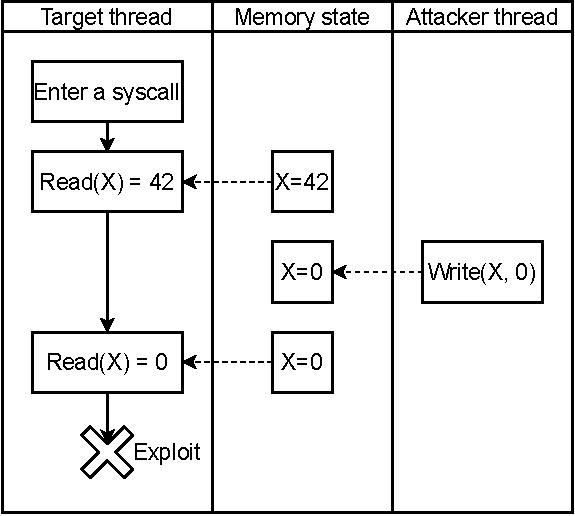
\includegraphics[width=.95\linewidth]{media/midas/doublefetch.pdf}
  \caption{Example of a double-fetch bug.}
  \label{fig:doublefetch}
\end{figure}

Double-fetch bugs occur when a privileged environment (such as the kernel)
reads untrusted memory multiple times, returning different values each time.
Such a situation is depicted in \autoref{fig:doublefetch}, 
where the value of \Code{X} in memory is changed by an attacker
between two reads by the target thread.
Exploiting such a bug requires a race condition i.e. accesses 
to memory in a particular order across threads.
A specific variety is the \emph{time-of-check to time-of-use}~(\tocttou) 
bug which occurs when the first fetch validates an object's value and
the second fetch uses the same object's value.
\tocttou bugs are widely studied in file systems, where the
API makes it possible to swap the file after validating the access
rights~\cite{payer2012protecting,
pu2006methodical, wei2010modeling, tsafrir2008portably,Garfinkel03}.
\tocttou bugs affect both kernel~\cite{jurczyk2013bochspwn, wang2018survey}
and dynamically-loaded driver code~\cite{cve201812633,cve201812633fix}.
Wang et al.~\cite{wang2018survey} showed that double fetches appear not only
in kernels, but wherever there is a trust boundary to cross (e.g.,
kernel---hypervisor~\cite{wilhelm2016xenpwn} and hardware---kernel
boundaries~\cite{lu2018untrusted}).


%%%%%%%%%%%%%%%%%%%%%%%%%%%
%\section{Attack vectors}
%\label{sec:threats}
%%%%%%%%%%%%%%%%%%%%%%%%%%%

% In this section, we describe the threat model for exploiting double-fetch
% bugs in the kernel and classify the possible attacks based on how the
% data is modified between vulnerable double fetches.

\section{Threat Model}
\label{sec:threatmodel}
%%%%%%%%%%%%%%%%%%%%%%%%%

% Nothing fancy -- the adversary is just trying to hack the system
% No black magic allowed
The attacker has access to a user account on the target machine. They can
execute arbitrary userspace code, including syscalls. Some of the system
calls have double-fetch vulnerabilities which the attacker wishes to exploit
(e.g., for privilege escalation).
The attacker may execute arbitrary sequences of syscalls on multiple CPU
cores in parallel, or concurrently on the same core.

\midas mitigates any unintended corruption or information leakage \emph{in the kernel}
or \emph{in other user processes} that arises through double-fetch bugs.
Hardware attacks such as Rowhammer~\cite{mutlu2019rowhammer}
or side-channels~\cite{KocherHFGGHHLM019}, and file-system TOCTTOU
attacks~\cite{payer2012protecting, pu2006methodical, wei2010modeling,
tsafrir2008portably} are out of scope.


\section{Attack Classification}
\label{sec:attacks}
%%%%%%%%%%%%%%%%%%%%%%%%%%%%%%%%%%

\begin{table}
  \centering

    \begin{adjustbox}{width=1.0\linewidth}
    \begin{tabular}{  l | l | l | l }
  \toprule
      & \textbf{Userspace} & \textbf{Kernel} & \textbf{Device} \\ \midrule

      % Note: this is a manually tuned fixup. multirow just sucks.
      & Intra AS     & User mapping          & DMA       \\
      \multirow{-2}{*}{\shortstack[l]{\textbf{Existing} \\ \textbf{mapping}}}
      & Cross AS     & Kernel mapping        & MMIO page     \\
      \midrule

      & \Code{mmap}  & \Code{mm\_populate}   & New           \\
      & \Code{clone} &                       & DMA/     \\
      \multirow{-3}{*}{\shortstack[l]{\textbf{New} \\ \textbf{mapping}}}
      & \Code{swap}  &                       & MMIO page              \\
  \bottomrule
  \end{tabular}
  \end{adjustbox}
  \caption{Attack vector classification for \tocttou exploits.}
  \label{tab:attack_class}
\end{table}

\midas guards data processed during a syscall's execution against concurrent modification.
We label the data fetched twice as vulnerable data.
In this section, we classify attacks based on two criteria: the
privilege level of the writer, and whether the mapping used for writing
exists at the time of the first read. \autoref{tab:attack_class} summarizes our
classification.
Importantly, this classification helps understand existing attacks and how to
protect against them, and where future attacks (bugs) may arise.
The device column corresponds to attacks where a device
(e.g., a network card, GPU, FPGA) is responsible for modifying vulnerable data.
Watson~\cite{watson2007exploiting} describes a subset of the
following attack vectors.

Existing userspace mappings to a page can be used to modify
vulnerable data which the targeted syscall is reading.
Userspace can directly write to a mapped page, irrespective of whether the mapping is
in the same address space or not.
% Watson~\cite{watson2007exploiting} called such attacks
% \emph{direct double fetch} attacks.
Alternatively, a concurrently executing syscall can also modify the
vulnerable data in a \emph{confused-deputy} attack.
When the attacker passes a pointer to the vulnerable data to
the syscall as a user buffer in which the syscall can return some
data, the kernel's write to the buffer can modify vulnerable data.
For example, the \Code{read} syscall takes an argument pointing
to a user buffer where the contents of a file will be copied to.
Another example is \Code{rt_sigaction}, where the kernel writes to
a user buffer pointed to by the \Code{oldact} argument.
In both of these attacks, the malicious write uses a userspace
mapping.
\emph{A protection mechanism must account for all userspace
mappings to pages containing vulnerable data at the time of the
targeted syscall's first read.}

Existing kernel mappings to a page also mapped in userspace can be
leveraged by an attacker in a confused-deputy attack.
Here, the attacker maps a file-backed page from the page cache into a
userspace process and then passes as an argument in this page to the
target syscall.
The attacker then triggers a concurrent \Code{write} syscall to modify the
vulnerable data using kernel mappings for the page cache
pages.
% This attack is called \emph{inception double fetch}~\cite{watson2007exploiting}.
% \mat{Did we call it inception double fetch?}
The kernel does not explicitly track kernel addresses mapping to a page,
but the file-system driver does explicitly find the page before writing to it.
\emph{A protection mechanism must instrument file-system
drivers to account for writes via kernel mappings to vulnerable data.}

The kernel might create new mappings to the vulnerable data
between the double fetches by the target syscall, bypassing any 
protective permissions installed by the transfer function in 
PTEs at the time of first read.
An attacker can call \Code{mmap} and \Code{clone} to create
a new mapping to the vulnerable data before writing to it.
% The first version is called a \emph{reflected double fetch}
% attack~\cite{watson2007exploiting}.
The page-table mapping might not be created at the time of the malicious
syscall, but lazily when the attacker writes to the vulnerable data
due to demand paging.
In a more involved variant, the attacker can use the kernel as a
confused deputy which touches the unmapped page and maps it in,
then writes to the vulnerable data.
In all of the above vectors, the function populating pages for a
process (\Code{mm_populate} on Linux) is creating the new mapping.
\emph{A protection mechanism must instrument any syscalls
and other kernel mechanisms which can create new mappings.}

Swapping may also create a new page-mapping.
If the attacker writes to a page that was previously swapped
to disk, but later swapped in to be read by the target syscall in
a different address space, the kernel might lazily reinstate
the attacker's mapping to the page.
\emph{The swapping mechanism must be protected.}

\midas protects against all of the previously-listed attack vectors.
In the absence of any other syscall which can create new userspace
mappings to vulnerable data, \midas' protection is complete
against writes from both user and kernel code.

Finally, a device might modify vulnerable data if it is either
allowed to DMA (direct memory access) to the page, or if the page is memory 
mapped (MMIO) and is actually backed by the device.
In the latter case, external factors can change the vulnerable
data.
Existing discretionary access control rules typically prevent users
(except a superuser) from mapping device-backed pages into their
address spaces.
Such users are also disallowed from configuring DMA devices.
Thus, device modifications to vulnerable data fall outside
our threat model and are not protected by \midas.
% The superuser may load arbitrary kernel code % via loadable
% % modules
% and confused-deputy attacks leveraging an incompetent
% system administrator are also outside the purview of our threat model.
However, \midas can be extended to protect against modifications by DMA devices
on processors supporting IOMMUs or similar methods for
access control~\cite{olsonbordercontrol}.
As a superuser can modify kernel code via kernel modules, protecting against 
attacks from this user falls outside of our threat model.


%%%%%%%%%%%%%%%%%%%%%%%%%%%
\section{\midas Design}
\label{sec:midas:design}
%%%%%%%%%%%%%%%%%%%%%%%%%%%

\midas maintains a single, core, \emph{invariant}:
\textbf{\emph{through a syscall's lifetime, every read to a userspace object
will return the same value}}.
By construction, the invariant guarantees that double-fetches in syscall
code will read the same data, \emph{eliminating \tocttou bugs}.
\midas maintains the invariant by tracking \emph{snapshots} of objects
when first accessed, lazily making \emph{copies} when the object is concurrently
written and accessing the correct copy on subsequent reads.
Copies are only maintained during syscalls' lifetimes, and are released as
soon as no syscall needs it.
Consequently, each userspace object has a single copy when no syscalls are
running.
The invariant also means that only accesses to userspace objects by the kernel
need to be protected.
Accesses to userspace objects from userspace and kernel objects by kernel
code remains unaffected.

\midas' implementation builds on the protection mechanisms provided by
existing virtual memory implementations.
On modern platforms, virtual memory protection is set up by the OS at
page granularity by setting bits in pagetable entries (PTEs).
These permission bits are checked by the hardware on memory access,
efficiently enforcing the permissions, and raising a fault when they
are violated.
For performance, \midas implements its invariant at page granularity, not object
granularity: when a syscall reads from userspace, every page touched by that
read is covered, not merely the bytes read.
Page-granularity protections are conservative compared to byte-granularity
protection and \midas maintains its invariant.
As a side-effect of its implementation, \midas does not distinguish
accesses to different parts of a page (intra-page false sharing).
False sharing leads to unnecessary page duplications, incurring performance
overhead on highly shared pages, but does not affect correctness.

For an object spanning multiple pages, \midas' design sequentially
protects each page before reading from it.
The leading pages containing the object are protected before the
later pages, allowing an attacker to potentially modify the later
pages before the syscall first reads them.
However, the attacker is prevented from modifying any of these pages
after the syscall's first read, ensuring that double fetches respect
the invariant.
If the syscall code contains a \tocttou bug, the modification will
be visible to the first fetch itself (which is used for checking for
validity of the data) and will lead to the data being rejected
straightaway.
\midas' invariant therefore prevent exploitation of double-fetch
vulnerabilities even when the fetched objects span multiple pages.
We elaborate on this case with an example in \autoref{sec:midas:design:discussion}.

A major requirement for \midas is to allow concurrent access to pages
by user/kernel code running in parallel with a syscall which reads from
the same pages.
This requirement prevents deadlocks and improves performance \textit{vis-a-vis}
a na\"ive design which blocks all other tasks writing to pages already
read by a syscall until the syscall completes.
The na\"ive design can deadlock because it introduces dependencies between
tasks for forward progress, which we illustrate in the following example
of a system with two tasks (A and B):
\begin{inparaenum}[\itshape i\upshape)]
  \item Task A issues a blocking syscall which reads a user page and blocks, then
  \item Task B writes to the same user page before issuing a syscall which
  resumes task A.
\end{inparaenum}
In this case, if Task A's read to the page preceeds Task B's write,
Task B will be blocked waiting for A to complete its syscall.
Task A will also remain blocked waiting for Task B's syscall,
introducing a circular dependency, leading to deadlock.
The na\"ive design also introduces unnecessary delays in other cases,
such as the one described below, again with two tasks (C and D):
\begin{inparaenum}[\itshape i\upshape)]
  \item Task C reads from a page and sleeps for a long while,
        but does not read from the page a second time, then
  \item Task D writes to the same page after task C has read from it,
        and blocks until Task C completes and is unnecessarily delayed.
\end{inparaenum}
A more performant approach is to duplicate the concurrently accessed page:
the copy is kept for task C for future fetches, and task D
can write to the original and proceed without delays.

\midas must maintain multiple versions of a page read by a syscall
to maintain its invariant in the face of concurrent writes.
\midas introduces \emph{snapshots} and \emph{copies} to keep track
of page versions.
Snapshots are logical views of the page's contents at a particular time,
while the actual contents are stored in one of many copies.
Each snapshot maps to a copy, allowing the contents of the page at the
time of creating the snapshot to be read.
If multiple snapshots are taken without intervening writes to the page,
these snapshots will map to a single copy, reducing \midas' space overheads
and performance overheads for creating copies.
\midas maintains a snapshot of every page when first read by a syscall.
On a double fetch by the same syscall, the copy mapped to the snapshot
is accessed, ensuring that the data read is the same as the first time.
The latest copy of the page is used for all writes, by the syscall as
well as from concurrently running tasks, updating the page as seen
from userspace.
%
\midas' design draws parallels to multi-version concurrency control
methods for databases based on snapshot isolation~\cite{WuALXP17}.
Transactions read from a snapshot of the database state from when
they started, and writes update the up-to-date state of the database.
%
\emph{Essentially, \midas is a multi-versioning system for pages where
syscalls read from immutable versions to prevent \tocttou bugs and
syscalls and userspace both write to a single mutable version
holding the latest state of the page.}

\subsection{Page State Machine}

\begin{figure*}[]
  \centering
  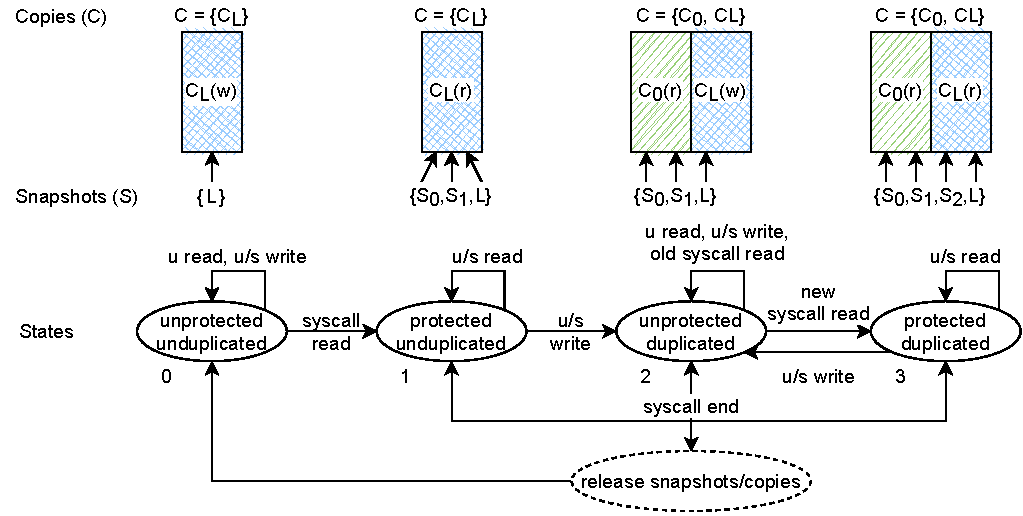
\includegraphics[width=0.9\linewidth]{media/midas/midas_states.pdf}
  \caption{State diagram for a page in \midas. Reads/writes from userspace/syscall
          code are marked (u)/(s) respectively. Shading is used to represent the
          mapping from snapshots to copies.}
  \label{fig:midas_states}
\end{figure*}

\begin{figure}[h]
  \centering
  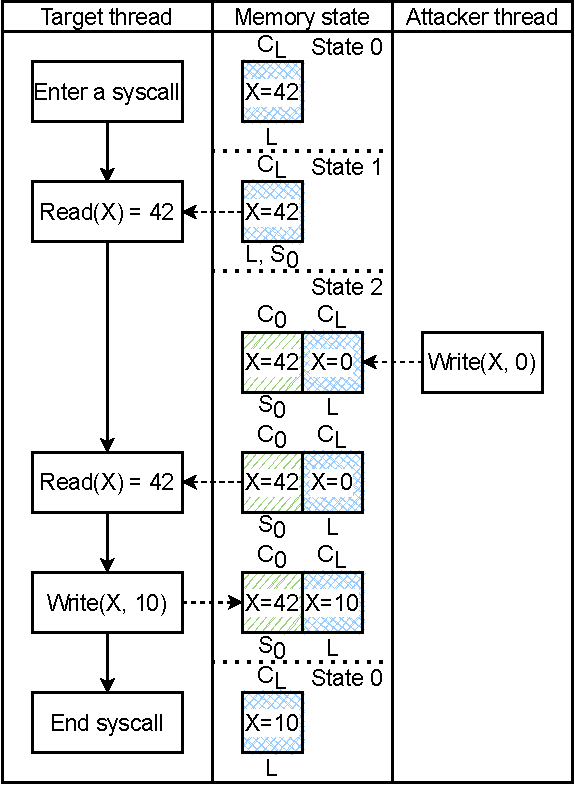
\includegraphics[width=0.95\linewidth]{media/midas/doublefetch_midas.pdf}
  \caption{Diagram illustrating \midas preventing exploitation of a
  double fetch of object \Code{X}.}
  \label{fig:doublefetch_midas}
\end{figure}

To track multiple versions of the contents of a page when being concurrently
accessed by numerous tasks, from userspace or during a syscall,
\midas implicitly maintains a per-user page state machine.
For a page, its corresponding state machine
\begin{inparaenum}[\itshape i\upshape)]
  \item tracks snapshots for currently executing syscalls which have read it,
  \item tracks copies of the page, and
  \item maintains the mapping between snapshots and copies necessary for providing
  the correct contents to subsequent reads. % by these syscalls.
\end{inparaenum}

\autoref{fig:midas_states} shows the state machine for a single page.
At every state, the page has two associated sets:
\begin{inparaenum}[\itshape i\upshape)]
  \item the copies set $C = \{C_L, C_0, \dots\}$ holds multiple copies of the page over time, and
  \item the snapshots set $S = \{L, S_0, S_1, \dots\}$ tracks logical versions of the page, each corresponding to one executing syscall and each mapping to a copy.
\end{inparaenum}
Reads from kernel code in a syscall use the \emph{snapshot's corresponding copy}.
Writes from user/kernel code and reads from userspace access the \emph{latest
copy} $C_L$, which is mapped in processes' address spaces.
All other copies are read-only (no matter what the original page protection is), and are used for providing snapshots to syscalls.
Read-only pages only use states 0 and 1, and writes lead to segmentation faults
(as they do on non-\midas systems).
Knowing which state the page is in allows \midas to differentiate between
faults due to \midas protecting pages and faults due to actual permissions
violations in userspace programs or the kernel.
The latest copy $C_L$ of read-only pages remains read-only in both
protected states (1 and 3).
In the following paragraphs, we describe how the state machine for a single,
writable user page transitions between its states, what triggers each transition,
and what changes are made to the copies and snapshot sets on a transition.
In \autoref{fig:doublefetch_midas}, we illustrate how the state machine protects the
syscall from \autoref{fig:doublefetch}.

\paragraph{State 0}
A page starts as \texttt{(unprotected, unduplicated)}.
In this state, there is a single copy $C_L$ and a single ``snapshot'' $L$.
The snapshot $L$ refers to the latest version of the page which changes
over time, and is the only mutable snapshot.
All processes where this page is mapped have unrestricted userspace read and write
access, and unrestricted kernel write access.
The remaining operation, a read from kernel code, triggers a transition to
State 1.
In \autoref{fig:doublefetch_midas}, the snapshot $L$ initially contains
the value $42$.

\paragraph{State 1}
The page in State 0 transitions to the \texttt{(protected, unduplicated)} state as soon as a syscall
reads from it.
\midas first marks the page's latest copy $C_L$ read-only in all processes,
trapping writes to the page but allowing concurrent userspace reads to continue.
A new snapshot, $S_0$ linked to this syscall is allocated for this page.
For the rest of its lifetime, this syscall will only read this page from this snapshot.
Both snapshots $S_0$ and $L$ refer to the same copy $C_L$ (shown by the
blue cross-thatch in \autoref{fig:midas_states}).
Prior to any writes to this page, any other syscalls which also read the page
get their own snapshots (e.g., $S_1$) all pointing to the single copy $C_L$.
The page's read-only status causes the hardware to fault on any write,
notifying \midas to transition the page to State 2.
In \autoref{fig:doublefetch_midas}, the page transitions to State 1 when
the syscall first reads it, and adds a snapshot $S_0$.

\paragraph{State 2}
A page in State 1 transitions to the \texttt{(unprotected, duplicated)} state
on any write from user or kernel code.
\midas duplicates the old contents of the page from copy $C_L$, creating a
read-only copy $C_0$ (shown by green shading in \autoref{fig:midas_states}).
Snapshots except $L$ (i.e. $S_0$ and $S_1$) previously mapping to $C_L$ are
mapped to the copy $C_0$.
The write then modifies the latest copy $C_L$, which is made writable again.
Note how, in this state, any read using the snapshots $S_0$ or $S_1$ reads
from the unmodified copy $C_0$ while writes directly affect $C_L$.
Certain syscalls such as \Code{rt_sigaction} both read and write from
the same user page.
A write by \Code{rt_sigaction} to the page it has previously read will update
the page's latest copy $C_L$, but not the duplicate copy $C_0$.
\midas' write policy ensures that the copy $C_L$ always holds the latest
contents of the page, up-to-date with all the writes to the page, from both user
and kernel code.
Further, \midas does not need to merge writes from userspace and syscall code
on a syscall's completion, since both directly modify the same copy $C_L$.
All other copies $C_i$ are immutable.
When the attacker writes to the page in \autoref{fig:doublefetch_midas}, the
page moves to State 2, linking the snapshot $S_0$ to a copy holding the
original value $42$.
The writes from both the attacker and the syscall itself both affect
the copy $C_L$, but the read from the syscall accesses the snapshot $S_0$
and reads the same value as the first time.


\paragraph{State 3}
A separate syscall subsequently reading the page in State 2 transitions
it to the \texttt{(protected, duplicated)} state.
The new snapshot, $S_2$, points to the latest copy $C_L$.
State 3 is similar to State 1, except that there are different copies of
the page used for reading by different syscalls.
The syscall for which $S_0$ was allocated will read from the copy $C_0$,
while the syscall for which $S_2$ was allocated will read from copy $C_L$.
On a write, the page transitions to State 2 and is duplicated again,
creating another copy $C_1$: snapshot $S_2$ maps to $C_1$ while
snapshots $S_1$ and $S_0$ continue to map to $C_0$.

\paragraph{Releasing snapshots}
\midas uses snapshots to enable a syscall to read the same data from a page
during its lifetime and releases snapshots when syscalls complete.
Releasing a snapshot is possibly accompanied by a state transition
and the release of the mapped copy.
If $S_i$ mapped to the latest copy $C_L$, \midas cannot free the copy
since userspace is using it.
In this case, the page must be in State 1 or 3, and $C_L$ is read-only.
After removing $S_i$, if $L$ is the sole remaining snapshot mapped to $C_L$,
\midas makes the page writable, moving to State 0 or 2 from State
1 or 3 respectively.
If $S_i$ is mapped to any other duplicate $C_i$, \midas frees the copy along
with the snapshot if $S_i$ is the last remaining snapshot mapped to $C_i$.
If the page was in State 2, $C_L$ was writable and unmapped by any snapshot,
so \midas changes the page to State 0.
This transition is shown in \autoref{fig:doublefetch_midas}, where the
snapshot $S_0$ and the copy $C_0$ are both discarded.
If the page was in State 3, $C_L$ was read-only and mapped by some other
snapshot, so \midas moves the page to State 1.
Recall that all snapshots $S_i$ except $L$ are immutable.
Any data written by the syscalls directly affect $L$.
Therefore, dropping a snapshot $S_i$ is trivial and does not require
writes from the syscall to be merged into the latest copy.

\subsection{Discussion}
\label{sec:midas:design:discussion}

\begin{table}
\begin{center}
  \begin{tabular}{  l  l }
  \toprule
    \textbf{System Call} & \textbf{Exemption reason} \\
  \midrule
    \Code{futex} & Relies on concurrent write \\
    \Code{execve} & Remaps address space \\
    \Code{write} & Invulnerable, improves performance \\
  \bottomrule
  \end{tabular}
\end{center}

\caption{System calls uninstrumented by \midas.}
\label{tab:except_syscall}
\end{table}

\paragraph{Correctness of syscalls directly updating snapshot $L$}
\midas' design lets all writes, including those from syscalls, to directly
update the latest copy of the page $C_L$ and this property maintains correctness
of system execution.
We now show that there is a valid, safe %\footnotemark
execution trace of a system not protected by \midas which generates the same
sequence of writes to the page, and therefore generates the same contents
of the page when the syscall ends.
%
We define a \emph{safe} trace as one that has no writes to vulnerable data between
double fetches by the kernel, and therefore does not trigger any existing
\tocttou bugs.
%
By showing that the final contents of memory after a \midas syscall has a
corresponding execution without \midas (which we assume to be correct)
leading to the same contents,
we can conclude that the execution of the \midas syscall is also correct.
For this proof, we assume that no syscall reads the same object after writing
to it (r-w-r pattern).
Such syscalls do not exist in the Linux kernel, and are discussed below.
Therefore, our syscalls write to an object after completing all of their reads
of that object.

% \footnotetext{A safe trace has no writes to vulnerable data between double fetches
% by the kernel, and therefore does not trigger any existing \tocttou bugs.}

Consider a page holding a single-byte object $O_0$, and the
sequence of operations to this byte during a \midas syscall be
$Ops = \{Op_0, Op_1, \dots \}$.
Each operation is a tuple $(r/w, k/u)$ specifying whether the
operation was a read or a write, and whether the operation was due to
a user or kernel instruction.
Suppose there was no attempt to exploit a \tocttou bug, i.e., between
any two read operations by the same syscall, there was no write to
this object.
% \mat{Second part of the conflict.}
% In case of the above mentioned scenario (1), which covers no concurrent
% writes, there are no writes to this object between any two read operations by
% the same syscall.
In this case, \midas reads the same value from its snapshot of the
object as is present on the latest version.
The same sequence of operations on a non-\midas system would be valid and
safe, since the object value does not change between the kernel's double
fetch and the syscall reads the same value on this system.

% \mat{Third part of the conflict.}
% Let us know focus on scenario (2) -- concurrent writes during a syscall's
% execution -- and
%
Assume there was an attempt to exploit a \tocttou bug:
a write $Op_1$ exists between two syscall reads $Op_0$ and $Op_2$.
\midas protects the syscall ensuring that $Op_2$ does not see the
effect of $Op_1$ by reading from a snapshot instead of the latest
copy $C_L$.
Since our syscalls are assumed to not contain any r-w-r pattern,
any writes by the syscall happen after $Op_2$.
Let us assume that the syscall's write is $Op_3$.
We can generate a valid, safe execution on a non-\midas system
by moving the attacker's write to after the last read by the
syscall, i.e., $Ops = \{Op_0, Op_2, Op_1, Op_3\}$.
The syscall in this system reads the same value both times, and
hence has the same execution as that in the \midas case.
The value of the object when the syscall completes is that
written by $Op_3$ in both cases (or that written by $Op_1$ when
the syscall does not have a final write).
Since the syscall has the same execution and the final value of
the object is the same, the execution of the \midas system
is the same as that of the non-\midas system.
In general, any trace of operations on a \midas system can
be translated  to a valid, safe trace on a non-\midas system
by moving malicious writes to an object to just after the last
double fetch of that object.
Multiple syscalls in \midas can therefore write to the same object
without affecting
correctness, because an equivalent, valid, safe non-\midas trace
exists where all of the writes have been postponed, in the same order
to after the double fetch reads.

\paragraph{Exemptions}
Syscalls such as \Code{futex} rely on user data changing between double
fetches to implement their functionality and cannot be protected by
\midas.
These syscalls are listed in \autoref{tab:except_syscall}.
The \Code{futex} syscall implements a fast synchronization mechanism
for userspace and relies on atomic writes from concurrent userspace
threads to update a condition the syscall is waiting for.
Subjecting a \Code{futex} syscall to \midas' invariant will prevent
it from ever waking up the waiting task.
Such syscalls cannot be protected by \midas, and we implement an
exemption list to prevent transitions in the state machines of pages read
by these syscalls.
The code for exempted syscalls must be manually inspected for double-fetch
vulnerabilities.
Crucially, exempting these syscalls from \midas' protection does not
affect the security of other syscalls containing double fetches.
Any writes from these syscalls are subject to the same rules described
in the state machine, and cannot break \midas' invariant.
\midas can also implement finer-grained exemptions based on syscall
parameters. Those were not necessary for Linux.
% Mat: the below is a bit stating the obvious, therefore commented.
%
% Other kernels may contain any number of
% syscalls which require exemption from \midas' protection, and
% they all need to be properly added to the exemption list.
% Finer grained exemptions based on syscall parameters can also be
% implemented, but was found unnecessary for Linux.
% A kernel where a majority of syscalls require exemption might not
% benefit from \midas' protection.


\paragraph{Syscalls with read-write-read patterns}
A (hypothetical) syscall that reads from an object, writes to it, and
then reads back the updated object cannot be protected using \midas.
\midas' invariant will ensure that the second read is identical to the first,
and does not reflect the intermediate write.
Such syscalls must remain exempt from \midas' instrumentation.
During extensive tests, we did not find any other syscall which exhibits this behavior in the Linux
kernel.

\paragraph{Syscalls with false sharing}
Another hypothetical type of syscall could struggle with \midas'
instrumentation due to false sharing.
Suppose a page contains two objects, $O_0$ and $O_1$, and a syscall
sequentially reads $O_0$ then $O_1$.
Due to \midas' invariant being enforced at page granularity and
false sharing of the page between these objects, \midas guarantees that
the value of object $O_1$ read is the same as what was contained when it
first read object $O_0$.
A syscall requiring the value of $O_1$ to change between these two
points in time would not work with \midas' protections.
Such a hypothetical syscall, requiring concurrent modifications to its
arguments, could exist to support some synchronization mechanism
similar to a \Code{futex} and can be safely exempt from \midas' invariant.
%
During extensive tests, we did not find any other syscall which exhibits this behavior in the
Linux kernel.


\begin{figure}[]
  \centering
  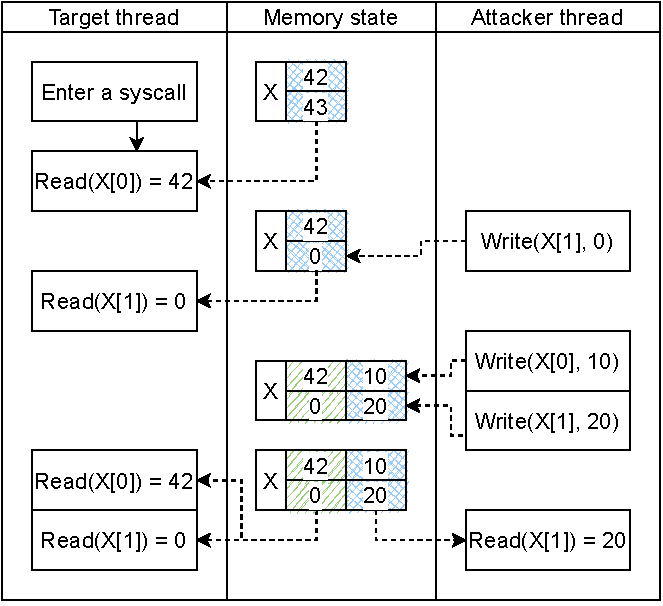
\includegraphics[width=\linewidth]{media/midas/doublefetch_midas_twopages.pdf}
  \caption{Diagram illustrating \midas preventing exploitation
  of a double fetch of an object \Code{X} spanning two pages.}
  \label{fig:copy_two_pages}
\end{figure}

\paragraph{Example: Objects spanning multiple pages}
\autoref{fig:copy_two_pages} shows \midas protecting a syscall which
has a double fetch for an object spanning multiple pages.
Here, the two pages containing the object \Code{X} are accessed as
\Code{X[0]} and \Code{X[1]}.
The attacker tries to attack the syscall by changing the value of the
second page:
\begin{inparaenum}[\itshape i\upshape)]
\item between the syscall's first reads of \Code{X[0]} and \Code{X[1]}, and
\item between the first and second fetches of X.
\end{inparaenum}
\midas ensures both fetches return \Code{X=(42,0)}.
Critically, any existing TOCTTOU bugs are not triggered since both fetches
read the same, possibly invalid, value of the object.
Note how the situation is identical to one where the malicious write
to \Code{X[1]} happens before the syscall starts.

\paragraph{Preventing deadlocks by design}
\midas' design is free of deadlocks, and exempts syscalls which
require violation of its invariant from triggering particular
state-machine transitions.
Userspace reads always succeed, using the latest copy $C_L$ of the
accessed page.
Writes from userspace and kernel code succeed directly if the
page is in State 0 or 2, and trigger a fault otherwise.
Handling these faults involves creating a new copy of the page and
setting the page writable.
Reading from kernel code involves creating a new snapshot and
setting the page read-only.
None of the aforementioned operations relies on other operations
on the same page to complete and all are finite time.
None of the operations on a page rely on operations on other pages.
A single, per-page lock can serialize operations on that page
and assure forward progress.

\paragraph{Detecting double fetches}
\midas' state machine for pages enables the precise detection of double fetch
bugs, turning it into an effective sanitizer and developer debugging tool in
addition to being an efficient mitigation.
When a syscall first reads from a user page, it creates a snapshot
of that page.
On future reads, the snapshot is used in order to maintain the
invariant.
While reading from a page, implementations must check
if a snapshot exists for the syscall: if yes, the snapshot is used
for the read, otherwise a new snapshot is created and then used
for the read.
The existence of a snapshot means the syscall had previously
read from this page and had then created this snapshot, implying a double
fetch.
Unfortunately, this approach is prone to false positives due to false sharing.
The two reads might read from the same page, but access entirely
disjoint bytes.
\midas currently reports double fetches at page granularity.
A precise sanitizer could maintain a bitmask of accessed bytes to
prune false positives.


%%%%%%%%%%%%%%%%%%%%%%%%%%%%%%%%
\section{\midas Implementation}
\label{sec:midas:impl}
%%%%%%%%%%%%%%%%%%%%%%%%%%%%%%%%

Our \midas prototype implements the state machine described in
\autoref{sec:midas:design} on Linux version 5.11, targeting the x86-64
architecture.
A page protected by \midas transitions between states on
either a kernel read to user memory, or when user or kernel code
writes to protected, read-only memory (see \autoref{fig:midas_states}).
\midas can be implemented on any operating system kernel that
\begin{inparaenum}[\itshape i\upshape)]
\item systematically uses transfer functions for reading from userspace, and
\item on any architecture which implements hardware-controlled access
control to memory through page tables.
\end{inparaenum}
The first requirement enables \midas to implement transitions on
kernel reads from user memory.
The Linux kernel uses the \Code{raw_copy_from_user} interface which
we instrument for our prototype.
The second requirement causes the hardware to raise a fault on
writes to \midas-protected pages,
directing execution on the processor to a pre-defined exception
handler in the OS.
Our prototype instruments Linux' fault handler in the function
\Code{handle_pte_fault} to implement the write-triggered transmissions
from states 2 and 4.
Overall, our prototype adds around $1,100$ lines of code and modifies
17.
Our design allows the changes to be mostly limited to the memory
subsystem, and in general does not require individual syscalls to
be modified.
Only one syscall~(\Code{clone}) required code modification.

\subsection{Tracking Page State}
%%%%%%%%%%%%%%%%%%%%%%%%%%%%%%%%

\begin{figure}[]
  \centering
  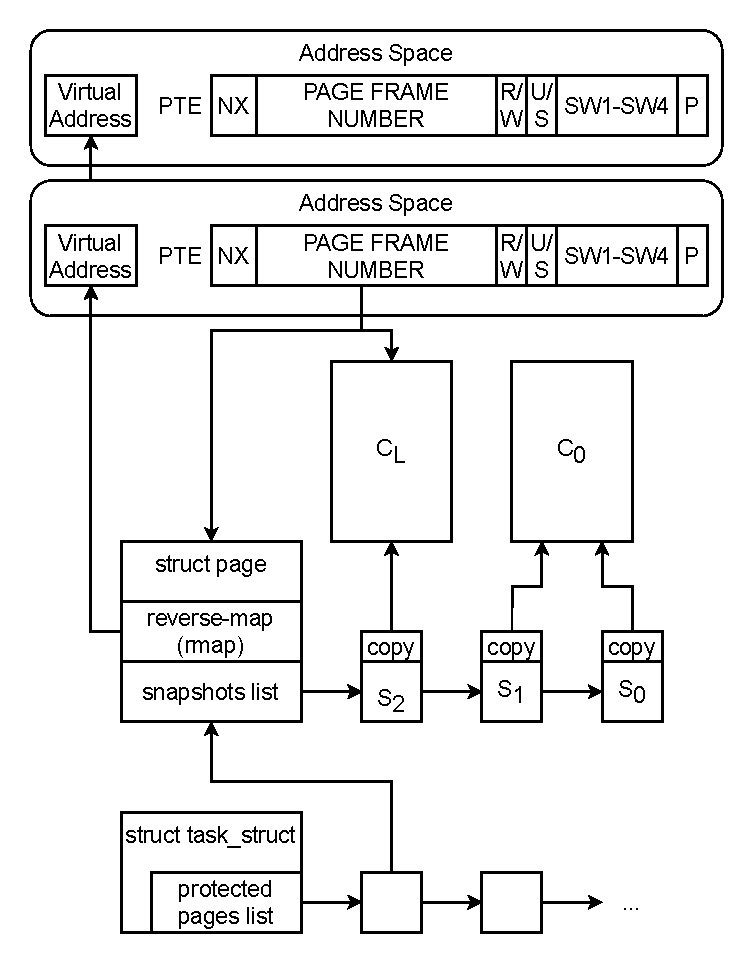
\includegraphics[width=\linewidth]{media/midas/book-keeping.pdf}
  \caption{Bookkeeping information for a page.}
  \label{fig:midas_bookeeping}
\end{figure}

\midas needs to track the state for every userspace page, including
its snapshot and copy sets.
\autoref{fig:midas_bookeeping} shows the data structures used to
track a page's state in our prototype.
Linux maintains a \Code{struct page} object for every frame of
physical memory.
We augment \Code{struct page}  with a list holding the snapshots
for this page, excluding the latest snapshot $L$.
Each snapshot has a pointer to its copy.
In the figure, the snapshots $S_1$ and $S_0$ share the copy $C_0$.
We are aware of the strong aversion of the
Linux kernel developer community towards increasing the size of
\Code{struct page}.
An alternate implementation can use a hashmap to
map from a page's frame number to its snapshots list or
reuse existing data members (e.g., \Code{struct list_head lru} which
can be used as a generic list by page owners).

Each pagetable entry for a user page in different address spaces
maps the copy $C_L$, enabling userspace to directly access the page
with reads (and writes for writable pages).
We use one software-controlled bit (SW3) in the pagetable entries
to track the protection status of the page, and another
(SW2)\footnote{The SW2 bit is alternatively used by the experimental Software Dirty Pages feature of
Linux, and cannot be run alongside \midas in our prototype.}
to track the original protections for the page.
SW3 is set whenever the page is in one of the two protected
states (1 and 3).
On a write-triggered protection fault, SW3 can be read to
efficiently determine if the fault was due to \midas' protection
mechanisms, triggering a state change, or due to buggy software
accessing a page with illegal permissions, triggering a signal to
the task.
Other architectures might have fewer software-usable
bits in the page table, and implementations of \midas would
require storing the protection status of pages in a separate data structure.
The duplication status of the page is implicitly encoded in the
snapshots: the page is duplicated when any of its snapshots
holds a pointer to a copy other than $C_L$.

Changing a page's protection state requires PTE updates
in all address spaces where the page is mapped.
The page's \Code{struct page} structure includes a reverse-map
listing for all of these pages, and the corresponding virtual
address in each.
Our prototype uses this mapping to change PTE permissions across
all address spaces for a page.


\subsection{Kernel Reads from User Memory}
%%%%%%%%%%%%%%%%%%%%%%%%%%%%%%%%%%%%%%%%%%

\begin{figure}[]
  \centering
  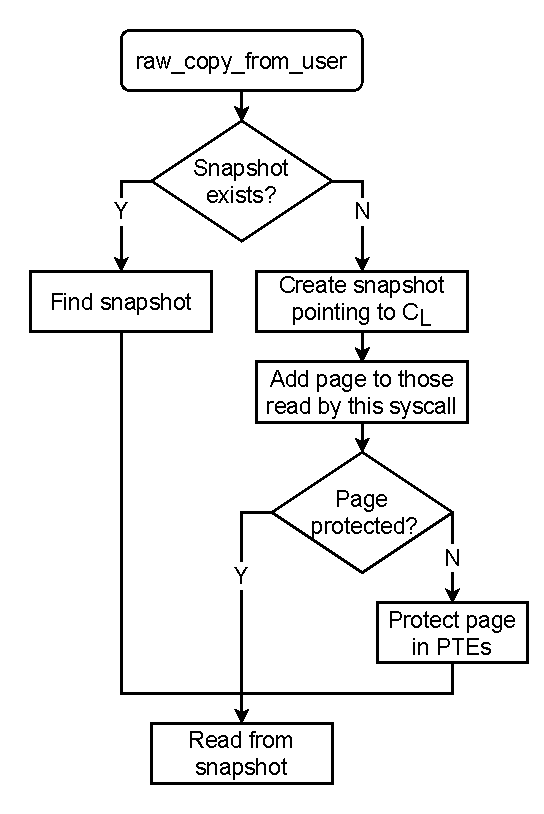
\includegraphics[width=0.8\linewidth]{media/midas/copy_from_user.pdf}
  \caption{Flowchart for a syscall using the transfer function
          \Code{raw_copy_from_user}
          for reading from userspace.}
  \label{fig:copy_from_user}
\end{figure}

Syscalls reading from user memory the first time triggers the
allocation of a new snapshot.
If the page is not protected (states 1 and 3), the read also
triggers a state change where the kernel protects the page
in all address space that it is mapped in.
\autoref{fig:copy_from_user} shows the flowchart of the steps
implemented by the kernel function \Code{raw_copy_from_user} for
reading from user memory.
This function also uses the kernel's \Code{mark_page_accessed}
interface to move the page to the ``Active'' state for the
kernel's swapping mechanism, making the page ineligible for being
swapped out.
We also implement \Code{get_user} and \Code{unsafe_get_user}
(used by the kernel for small reads) as a call to \Code{raw_copy_from_user}.

\paragraph{Exemptions}
Our prototype \midas kernel exempts a couple of functions
from \midas' invariant (in addition to those described in
\autoref{sec:midas:design:discussion}), and these functions are
therefore not instrumented
to follow the aforementioned steps while accessing userspace
memory.
First, \Code{raw_copy_from_user_inatomic} is a special
transfer function used by the kernel to
read user memory in special situations such as a kernel
oops\footnote{A kernel oops is triggered when the kernel detects a
problem while running which can affect its proper functioning, such
as corrupted data structures.
A more severe version, a kernel panic, causes the kernel to stop
executing, expecting data loss or damage if it does.}
where the kernel reads user memory to provide a backtrace.
In this severe situation, the kernel's goal is to collect debug
information before its imminent termination and no \tocttou protection
is needed.
Second, we also exempt the \Code{write} system
call's reads from user memory from instrumentation.
The \Code{write} syscall takes three arguments: a
file descriptor passed as a register, a pointer to a user
buffer and a count of bytes to be written to the file.
While the write to the file's pages is sensitive, and
\midas takes care to ensure that it follows the page state
machine, the read from userspace is not.
The syscall reads from userspace only once, and its data
is only used for copying into the file.
An attacker who modifies the user buffer concurrently with
the syscall only manages to change the contents written to
file, which it could have done anyway since it has access to
this buffer.
A kernel developer can similarly exempt other syscall which
they can prove to be secure from double-fetch bugs.


\subsection{Handling Faults}
%%%%%%%%%%%%%%%%%%%%%%%%%%%%

\begin{figure}[]
  \centering
  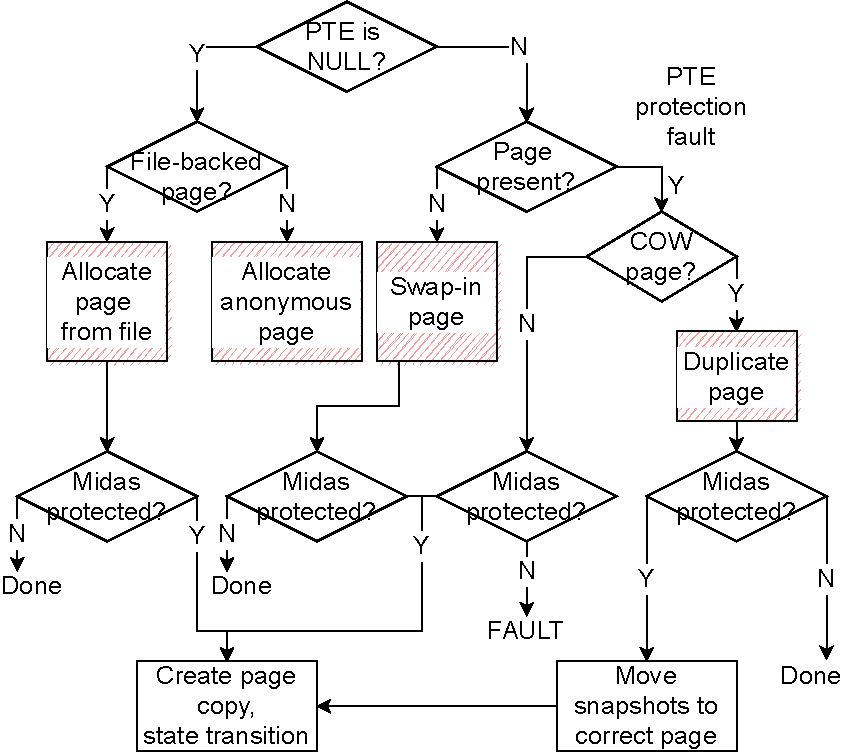
\includegraphics[width=\linewidth]{media/midas/pagefault.pdf}
  \caption{Flowchart for handling a page fault. Shaded
          operations are unmodified.}
  \label{fig:fault_handling}
\end{figure}

\begin{figure}[]
  \centering
  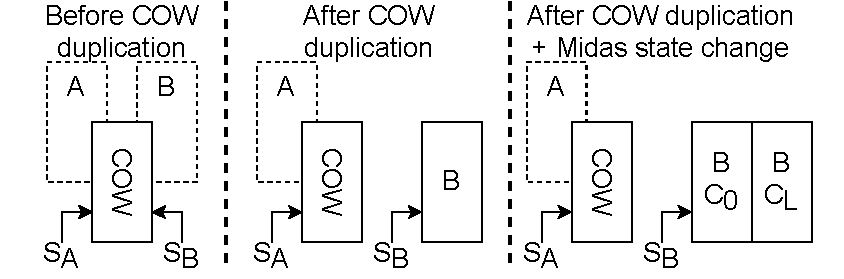
\includegraphics[width=\linewidth]{media/midas/pagefault_cow.pdf}
  \caption{Flowchart for handling a page fault to a COW page.}
  \label{fig:fault_handling_cow}
\end{figure}

The memory management unit generates a fault when kernel or user code accesses
a page without having the correct permission in the corresponding PTE.
\midas marks writable pages read-only to protect them in
states 1 and 3, allowing the kernel to detect writes to these pages.
A common OS mechanism, copy-on-write (COW) pages, also uses
permissions in the PTE to detect when COW pages need to be copied.
The PTE's present bit are used to store pointers to file-backed pages
when they are swapped to disk.
\autoref{fig:fault_handling} shows the flowchart implemented by
\Code{handle_pte_fault} to handle faults for userspace addresses.

The page-fault handler first checks if the PTE is NULL, and if so
knows that it must allocate a page.
If the required page is anonymous, the page can be allocated as usual.
Otherwise, for file-backed pages, the handler has to check if the
page is already in a protected state (states 1 and 3) by reading
the SW3 bit of the PTE and if so, transitions to the required state
and allocates a new copy.
Pages in states 0 and 2 can be directly mapped, and subsequently
accessed.

For non-NULL PTEs, the handler checks if the PTE indicates that the
page is present.
Non-present pages need to be swapped in.
After finding the page, \midas then checks if the page was previously
swapped in by any other task and is now in a protected state.
For protected pages, \midas implements the required state change based
on whether the faulting access was a read or a write.

In the remaining case, faults for a present page indicate a
permission fault (for example, a write to a read-only page).
If the page is not a COW page, the handler then checks if the page
is in a protected state by checking the SW3 bit.
If the page was protected, a new copy is allocated and the page
transitions to the following state.
For non-protected pages, however, the fault implies a real access
violation, sending a signal to the process.

COW pages represent separate virtual pages from different
address spaces mapped to the same physical page.
An example of a COW page protected by \midas is shown in
\autoref{fig:fault_handling_cow}, where logically-separate pages A and B
are actually mapped to the COW page.
COW pages cannot be in states 2 or 3, since they cannot have multiple
\midas copies.
COW pages in state 0 can be dealt with by the kernel's standard
duplication method (not \midas' duplication).
For a COW page in state 1, its list of snapshots can correspond to
reads from syscalls for threads in different address spaces.
In \autoref{fig:fault_handling_cow}, we show snapshots $S_A$ and
$S_B$ corresponding to syscalls for threads in different address
spaces (containing A and B respectively).
These snapshots correspond to different logical pages, but are
all squashed into the snapshots list of the single COW page.
Therefore, after the kernel duplicates the COW page (new page
B created, in \autoref{fig:fault_handling_cow}), \midas moves
the snapshots for the faulting process ($S_B$) to the new page.
Here, \midas also updates the protected page list in the
affected syscalls' \Code{task_struct}s so that these structures
correctly refer to the new page.
Finally, the new page is transitioned to its next state to allow
for the write to occur, creating a new copy ($C_0$) for the
snapshot $S_B$ to read from.

We ensure that \midas' modifications to the fault handler
correctly handle concurrent faults and do not cause additional
nested faults.
During concurrent faults for the same page, only one thread
changes the page's state whereas the other directly uses the new
state.
The kernel's split page-table lock is reused to serialize state
changes.
We also ensure that the only additional accesses to user memory
within the handler (used for duplication) happen when the page
is assured to be in memory and correctly mapped.
All nested faults are therefore caused by existing kernel code
and do not interact with \midas' modifications.

\subsection{Syscall Completion}
%%%%%%%%%%%%%%%%%%%%%%%%%%%%%%%

On syscall completion, \midas cleans up snapshots allocated for
the syscall by instrumenting the end of \Code{do_syscall_64}.
\midas goes through the list of all the pages for which the
executing syscall has a snapshot, and frees those snapshots.
For snapshots which were the last to point to a copy, that
copy is also freed.


\subsection{File System Writes}
%%%%%%%%%%%%%%%%%%%%%%%%%%%%%%%

\midas instruments file-system writes to protect the kernel
from modifications via kernel mappings.
When a \Code{write} syscall writes to a file, it actually
writes to copies of pages of the file stored in memory within
a page cache.
In the spirit of abstraction, the kernel does not directly write to
these pages, but calls the relevant file-system (FS) driver instead.
The FS driver will access the page using kernel mappings when writing to pages in the page cache.
Since \midas only protects userspace mappings for protected pages,
writes by FS drivers will not raise a fault.
To comprehensively protect the page, any implementation needs to
instrument FS drivers' write functions.
Fortunately, FS drivers provided with the kernel follow a simple
recipe: for pages not in the page cache, the driver executes
FS-specific code to read the page into the page cache and then
call a generic function (\Code{generic_file_write_iter}) to actually
write the data into the page.
Instrumenting this generic function, therefore, protects the kernel
for a wide range of common file-systems (including ext4, nfs and
ntfs). \footnote{A more comprehensive list of kernel-provided FS drivers
protected via \Code{generic_file_write_iter} includes v9fs, ADFS, AFFS,
AFS, BFS, CIFS, eCryptfs, extFAT, ext2, F2FS,  FAT, FUSE, HFS, HFS+,
hostfs, HPFS, JFS, JFFS2, Minix, NILFS2, OMFS, OrangeFS, ramfs, ReiserFS,
SystemV, UBIFS, UDF, UFS, VboxSF, shmem.}
The added instrumentation checks whether the target page is
protected, and if so, transitions it to the next state and
creates a copy of the page before writing to the latest copy.

Our current prototype does not, however, protect out-of-tree drivers
which are not distributed with the kernel if they do not use the
\Code{generic_file_write_iter} function.
A user with superuser privileges can load a insecure module implementing a
FS driver which does not implement \midas checks.
A malicious superuser is, however, outside our threat model.
% Mat: IMO a very weak argument and always the case, so rather than waste
% precious time here, I've commented out the below as it distracts from our key
% argument IMO.
%
% A more reasonable threat involves a sysadmin unwittingly loading a
% insecure driver which a non-privileged user can then use to
% exploit a \tocttou bug.
% One solution would be for the kernel to inspect the relocations table of
% a new module while loading it to see if it uses \Code{generic_file_write_iter}
% and raising a warning if it does not.


\subsection{New Mappings to Protected Pages}
%%%%%%%%%%%%%%%%%%%%%%%%%%%%%%%%%%%%%%%%%%%%

Our \midas prototype preserves the state machine for user pages
across operations which create new mappings to a page to prevent
attacks which rely on mappings being created between double fetches.
The \Code{mmap} syscall is responsible for creating new virtual
memory mappings for processes, and requires instrumentation.
When \Code{mmap} is called with the \Code{MAP_POPULATE} flag, or
on the first access to the page, the \Code{mm_populate} function
is responsible for actually mapping the correct page in the
page table.
In our prototype, we check if the page being mapped is protected,
and if so, correctly protect the new mapping too.
Another syscall, \Code{clone}, duplicates a process' address space
when called without the \Code{CLONE_VM} flag, creating new mappings
to pages.
We instrument \Code{clone} to ensure that new mappings for protected
pages are also correctly protected.


\subsection{Discussion}
%%%%%%%%%%%%%%%%%%%%%%%

\paragraph{Optimizations on capable hardware}
To protect a page in an address space, a \midas implementation
needs to change the permissions in the page table for that page.
Modern CPUs cache virtual memory translations in per-core
Translation Lookaside Buffers (TLBs) which need to be (partially)
flushed on page-table updates (TLB shootdown).
On most CPUs, the core updating permissions will perform a global
shootdown to ensure that other TLBs for cores executing in the
same address space are also updated.
Implemented with inter-processor interrupts, global shootdowns
are expensive.
In our evaluation, 21\% of the runtime of the load generator
\Code{bombardier} used for stressing the Nginx server was spent
performing TLB shootdowns when running on the \midas kernel.

A more efficient solution would be to have special hardware support
for invalidating TLB entries globally, not just on the executing
core.
The AMD64 architecture manual~\cite{amd64prog} lists such an instruction
(\Code{INVLPGB}), though it is yet to be implemented in any commercially
available x86 processors.
The ARM v8-A architecture manual~\cite{armv8a} lists similar instructions
\Code{TLBI ASIDE1}\texttt{\textbf{IS}} and \Code{TLBI ASIDE1}\texttt{\textbf{OS}} which invalidate all PTEs
of a page within a cluster of cores but not for cores in other clusters
(Inner Shareable Domain) and cores across clusters (Outer
Shareable Domain) respectively.

Alternate architectures~\cite{0003BOBFP21midgard,ChaseLFL94SASOS} with a single,
system-wide translation table
would also benefit \midas by having a single page table to
update instead of multiple page tables for each address space a page
is mapped in.

\paragraph{Porting to other OSs}
\midas can provide \tocttou protection on other operating systems by
tracking the states of each page and implementing state transitions
as required.
OSs track page state in per-page state structures,
such as \Code{vm_state_t} for BSD-based OSs (*BSD) such as FreeBSD and XNU.
An implementation on these OSs must instrument the
read transfer function(\Code{copyin} for *BSD) to transition to states 1 and 3.
The OS' fault handler (\Code{vm_fault} on *BSD) will trap on writes to
protected pages, and needs to be modified to implement the required page
duplication and state change.

The remaining OS modifications for \midas support depends on
the OS' features.
If an OS allows userspace to map file pages, filesystem code to write
to these page needs to be modified.
Other syscalls which create/modify mappings to userspace pages will
also have to be instrumented to ensure that the new mapping respects the
page's state.
Such modifications are OS-specific, making it difficult to recommend
a generic methodology.


%%%%%%%%%%%%%%%%%%%%
\section{Evaluation}
%%%%%%%%%%%%%%%%%%%%

In this section, we emperically verify \midas' ability to mitigate
a known double fetch vulnerability, and quantify \midas' overhead on
workloads with different characteristics including both compute-bound
applications which rarely use syscalls and a mix of syscall-heavy applications
which heavily rely on the kernel's performance.

\subsection{Mitigation of CVE-2016-6516}
%%%%%%%%%%%%%%%%%%%%

\definecolor{mygreen}{RGB}{62, 123, 49}
% \begin{minipage}{\linewidth}
\begin{lstlisting}[language=C, escapeinside={<@}{@>},
                  basicstyle=\ttfamily, frame=single, numbers=left,
                  captionpos=b,
                  label=lst:cve-2016-6516,
                  caption={CVE-2016-6516: Vulnerable double fetch in \Code{ioctl_file_dedupe_range}.
                          Lines in green show the fix and testing code.},
                  float]
  //First fetch
  if(get_user(count,&argp->dest_count))
  {...}
  //Using first fetch
  size = offsetof(..., info[count]);
  //Secong fetch
  same = memdup_user(argp, size);
<@\texttt{\color{mygreen}{+ \textit{//Added check for bug}}}@>
<@\texttt{\color{mygreen}{+ \textbf{if}(same->dest\_count != count)}}@>
<@\texttt{\color{mygreen}{+ \ \ printk("Bug triggered");}}@>
<@\texttt{\color{mygreen}{+ \textit{// Fix: copy over original count}}}@>
<@\texttt{\color{mygreen}{+ same->dest\_count = count;}}@>
  //Using second fetch
  ret = vfs_dedupe_file_range(file,same);
\end{lstlisting}
% \end{minipage}

CVE-2016-6516 is a known vulnerability in kernels prior to version
4.7 in a file-system \Code{ioctl}.
The vulnerable code is shown in \autoref{lst:cve-2016-6516} and is
triggered when the value of the \Code{dest_count} object differs between
the two fetches (in lines 2 and 7).
\Code{memdup_user} uses the value from the first fetch for allocating a buffer
and copying in an array of descriptors from the user in line 7.
\Code{memdup_user} also contains the second fetch of \Code{dest_count}
which is later used in the function \Code{vfs_dedupe_file_range}.
An attacker who increases the size of \Code{dest_count} between the
two fetches will cause the kernel to access the copied array out-of-bounds,
causing a heap buffer overflow.

For verifying \midas' defense, we introduce a non-faulting assertion
check into the function~(lines 9--10) and run a known
exploit.\footnote{\url{https://github.com/wpengfei/CVE-2016-6516-exploit/tree/master/Scott\%20Bauer}}
The condition checks whether the fetched value of the user object (\Code{dest_count})
had changed, indicating a successful attack, and prints a message.
Finally, we re-introduce the fix for the bug (line 12), fixing the value of
\Code{dest_count} in \Code{same} to that from the first fetch.
In this setup, we can detect when the conditions for triggering the bug are met,
but also revert to a correct state allowing the kernel to safely
continue.
The exploit was able to successfully trigger the bug on the baseline kernel
every time over 10 runs.
With \midas enabled, the exploit was never triggered, i.e., both fetches
returned the same value on every call.\\


\subsection{Performance evaluation}
\label{sec:perf}
%%%%%%%%%%%%%%%%%%%%

We evaluate \midas on
\begin{inparaenum}[\itshape i\upshape)]
\item microbenchmarks targeting specific common syscalls,
\item workloads from two benchmark suites: the NAS Parallel
    Benchmark (NPB)~\cite{npb} and select workloads
    from the Phoronix Test Suite (PTS)~\cite{pts}, and
\item the webserver Nginx.
\end{inparaenum}
NPB includes compute-intensive multiprocessing workloads with a
low, but non-negligible syscall rate.
NPB therefore demonstrates the ability of \midas to
scale to systems where pages are protected across numerous
address spaces.
PTS includes a variety of benchmarks, both compute bound and
I/O bound representative of both desktop and server workloads.
PTS includes syscall-heavy applications with varying degrees
of parallelism.
The Nginx webserver is capable of both high request service rates
and scalability with multiple worker processes.
We do not include the SPEC CPU2017 benchmarks
as they are heavily compute bound and designed to isolate userspace
performance without syscalls, and are impervious to kernel performance.
SPEC benchmarks would unfairly bias performance in favor of
\midas.

The testbench for the evaluation consists of a desktop machine
with an 8-core Intel i7-9700 processor and 16GB DRAM running
Ubuntu 20.04 LTS. This configuration and CPU is commonly used on desktop
machines and workstations.
%
To eliminate the effect of dynamic frequency and voltage
scaling (DVFS), we set the processor to run at constant
frequency of 3.0GHz which is this model's base frequency.
In the \emph{baseline} configuration, we run the testbench
with the mainline kernel v5.11 available from Ubuntu's package
repository.
The \emph{\midas} configuration runs our prototype \midas kernel
also based on kernel v5.11.
For particular benchmarks, we also run the \emph{\midas{+}write}
configuration which also runs our prototype \midas kernel
but instruments all syscalls including \Code{write}.

\begin{figure*}[!t]
  \centering
  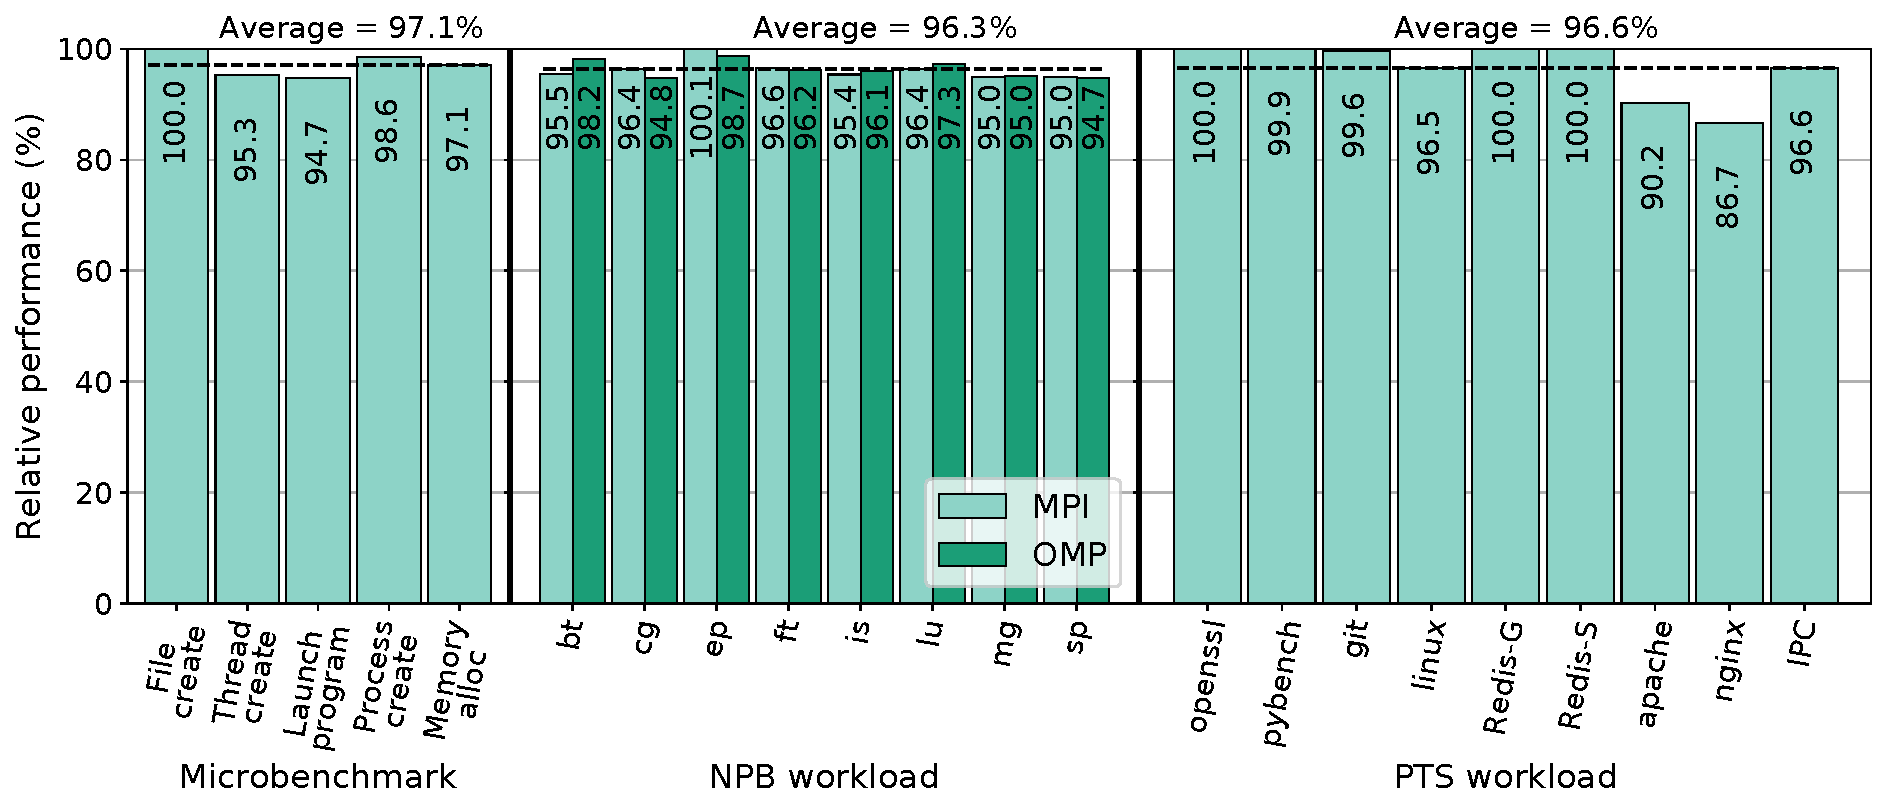
\includegraphics[width=\linewidth]{media/midas/midas_performance.pdf}
  \caption{\midas' performance on microbenchmarks, NPB and PTS benchmarks
          relative to the baseline kernel.}
  \label{fig:midas_performance}
\end{figure*}

\begin{table}
  \centering
  \begin{tabular}{l l}
    \toprule
    \textbf{Microbenchmark} & \textbf{Top syscalls used} \\
    \midrule
    File creation & \Code{openat}, \Code{fstat}, \Code{write}, \Code{close} \\
    Thread/Process creation & \Code{mmap}, \Code{clone}, \Code{exit}, \Code{wait} \\
    Program launch & \Code{mmap}, \Code{execve}\Code{readlink}, \Code{openat} \\
    Mem alloc & \Code{brk} \\
    \bottomrule
  \end{tabular}
  \caption{Prominent syscalls used by OSBench microbenchmarks.}
  \label{tab:osbench_syscalls}
\end{table}

\paragraph{Microbenchmarks}
%%%%%%%%%%%%%%%%%%%%%%%%%%%%%%%%%%%%
We test \midas on microbenchmarks from
OSBench~\cite{osbench}.
The programs use \Code{libc} interfaces such as \Code{fopen},
\Code{pthread_create}, \Code{fork} and \Code{malloc} for creating files,
threads, processes and for memory allocation respectively.
\autoref{tab:osbench_syscalls} lists the prominent syscall usage
for these workloads.
\autoref{fig:midas_performance} shows \midas' performance
(time per operation)
on OSBench relative to the baseline kernel, with overheads ranging from
zero to 5.3\%.

\paragraph{NAS Parallel Benchmarks}
%%%%%%%%%%%%%%%%%%%%%%%%%%%%%%%%%%%%
NAS Parallel Benchmarks (NPB)~\cite{npb} is a benchmark introduced by
NASA.
NPB consists of several parallel programs using different communication
patterns and is available for two frameworks for parallel programming:
OpenMP and MPI.
OpenMP~\cite{dagum1998openmp} is a compiler extension that splits a
program's execution to multiple threads.
All threads still use the same address space, keeping the overhead minimal.
MPI~\cite{snir1998mpi} implements parallel execution by launching multiple
processes which communicate by message passing.
The two technology stacks have different frequency of syscalls due to
different communication methods.
Communication through kernel syscalls for either stack will incur overhead
due to \midas' protection.
Additional global TLB shootdowns (for snapshot synchronization) added by
\midas will also affect the performance of such parallel benchmarks.

We run NPB benchmarks of class A on our testbench, executing
4 threads or processes in parallel.
The benchmarks' runtime varies between 10 seconds and 8 minutes,
and are all long enough for the kernel to reach equilibrium.
Certain benchmarks require a parallelism number which is a perfect square.
On our 8-core CPU, having 4 compute-bound threads/processes instead of 16 allows
all threads to run without time sharing.
\autoref{fig:midas_performance} shows \midas' performance for both MPI and OpenMP,
normalized to the performance of the baseline system with the same parallelization
framework.
On average, \midas achieved $96.3\%$ of the baseline system's performance on
both frameworks.
\midas' performance for the \Code{ep} (Embarrassingly Parallel) benchmark is
closest to that of the baseline, since it has low communication overheads.
\midas shows low overhead ($3.7\%$) for compute-intensive, parallel workloads.


\paragraph{Phoronix Test Suite}
%%%%%%%%%%%%%%%%%%%%%%%%%%%%%%%%
The Phoronix Test Suite (PTS)~\cite{pts} includes a large set ($>500$) of
open-source benchmarks, of which we have chosen a range of benchmarks
suitable for evaluating both desktop and server performance.
We bias the selection to benchmarks that require (heavy) kernel activity to
test the overhead of \midas' instrumentation.
A sole benchmark, OpenSSL, is included to represent single-threaded,
compute-bound workloads for which kernel performance is less relevant.
The benchmarks are also varied, ranging from single-threaded (Pybench) to
multi-threaded, multi-process workloads (Apache).
At the extreme, we have an IPC benchmark transferring tiny, 128-byte
buffers between processes which spends all of its time in syscalls
and whose performance is entirely dependent on kernel IPC performance.

We plot \midas' performance relative to the baseline kernel on
these benchmarks in \autoref{fig:midas_performance}, roughly ordering
workloads in increasing order of syscall dependence from left to right.
For benchmarks for which PTS reports runtime, we compute the inverse
of the runtime as performance.
Benchmarks with low syscall frequency such as OpenSSL,
Pybench and Git have correspondingly low dependence on kernel performance.
Accordingly, these benchmarks see a negligible overhead when running
on our prototype kernel.
The benchmark titled ``Linux'' represents compilation of the Linux kernel.
While compilation is mostly compute bound, compiling the Linux kernel requires
accessing a large number of source files, resulting in the creation
of a large number of compiler processes each of which read and create
files.
\midas experiences a small, but non-negligible overhead of $3.5\%$ on this workload.
Redis requires syscalls for receiving and replying to requests, but
processes its transaction entirely in-memory.
Our evaluation prototype achieves practically identical results as the baseline,
highlighting the final prototype's competitive performance.
The webservers, Apache and Nginx require network and file-system I/O,
and rely heavily on syscall performance.
We see that Nginx, which is a higher-performance webserver, sees a larger
overhead.
IPC, which implements 128 byte transfers between
two processes over a TCP connection, is almost entirely bound by kernel
performance and sees a performance overhead of $3.4\%$ on \midas.

Our prototype \midas kernel benefits significantly from
exempting particular, proven-safe syscalls from instrumentation.
While we exclude \Code{write}-like syscalls from \midas because they
are not vulnerable to double-fetch bugs, we also evaluated the
performance cost of an unoptimized implementation (\midas{+}write)
which also instruments these syscalls.
To highlight the worst-case performance of the unoptimized implementation,
we evaluate the performance of the IPC benchmark on \midas{+}write due
to its high frequency of \Code{write} syscalls.
With \midas{+}write, the performance of the IPC benchmark falls to
$12.6\%$ of the baseline, a further degradation of $84\%$ compared
to \midas, showing that developer effort towards properly exempting
frequently called \emph{safe} syscalls from \midas protections is crucial
towards for implementations to maintain competitive performance
compared to the baseline.

\paragraph{Memory overhead}
Our prototype incurs memory overhead due to metadata, tracking page snapshots
and copies.
At any instant, the memory overhead mainly depends on the number of executing
syscalls (limited by the core count) and the number of page copies for these
syscalls.
On average, for every 1000 syscalls issued by the PTS benchmarks, our prototype
created 236 snapshots (32B each) and 54 copies (4KB each).
We can see that the occurrence of copies is low, resulting in negligible
memory overhead.

\subsection{Overhead breakdown}
%%%%%%%%%%%%%%%%%%%%

\begin{figure}
  \centering
  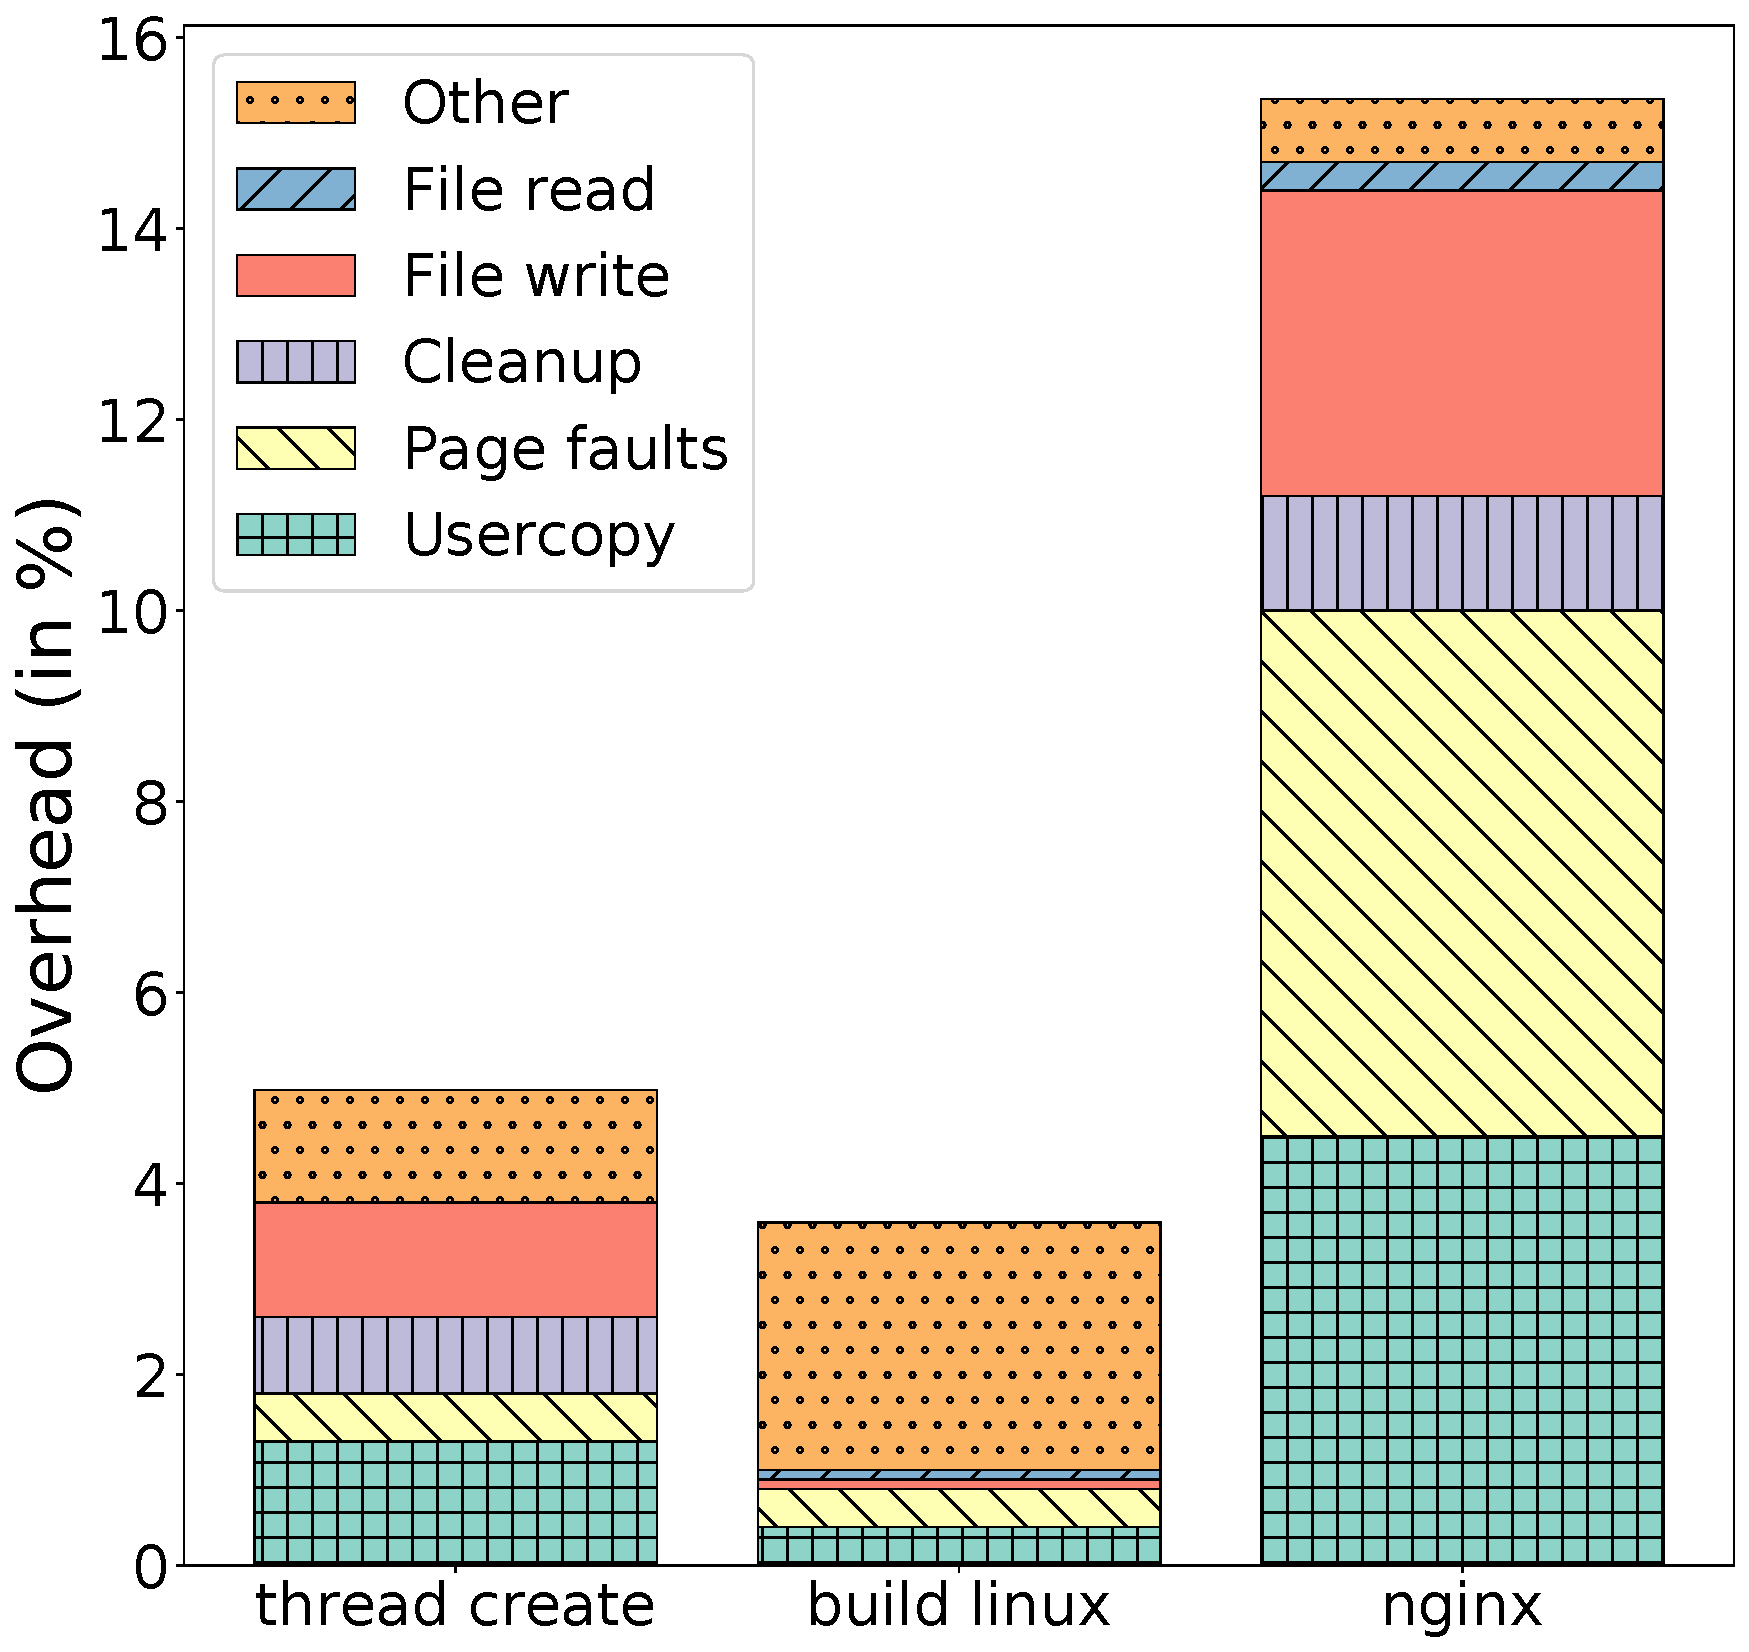
\includegraphics[width=\linewidth]{media/midas/overhead.pdf}
  \caption{Classification of overheads for various benchmarks due to \midas.}
  \label{fig:overhead_class}
\end{figure}

In this section, we explore the sources of \midas' overhead by analyzing
\Code{perf} traces for three workloads: thread creation from OSBench, linux
compilation from PTS and Nginx.
We aim to classify overheads into the various kernel function we instrumented:
\begin{inparaenum}[\itshape i\upshape)]
\item user copy in transfer function,
\item page duplication on page fault,
\item metadata cleanup on syscall end, and
\item filesystem operations.
\end{inparaenum}

To estimate the time spent in each function, we create FlameGraphs for
each workload\cite{GreggFlameGraph} using samples of processor state, including
the call stack, collected over 30 second periods by \Code{perf record}.
After identifying one binary for the workload from the FlameGraph, we estimate
the overhead for a function as the difference in execution time attributed to
that function between the baseline and \midas systems.
The total overhead is estimated from the throughput figures obtained from
\autoref{sec:perf}.

\autoref{fig:overhead_class} shows the breakdown of overheads for three
workloads.
As expected, metadata tracking and duplication causes most overheads
for the user copy and fault handling functions respectively.
The results for the Linux build breakdown differs 
from the other workloads
in the large portion of
the unaccounted overhead (labelled ``Other'').
This anomaly stems for the fact that Linux's compilation runs a large number (1000s)
of processes, of which the compiler accounts for less than~50\% of the
total execution time.
The reported breakdown accounts for overheads on the compiler, but not
all the other processes.

Both page faults and user copies cause state changes for a page, and thereby
change the page's access permissions in the PTE.
The resulting TLB flush accounts for 0.3\%, 0\% and 1.1\% overhead for
thread creation, compilation, and Nginx respectively.
The load generator \Code{bombardier} used for loading Nginx, however, sees
a much larger overhead for TLB flushing, accounting for
21\% of its execution time.

\subsection{Case study: Nginx}
%%%%%%%%%%%%%%%%%%%%

\begin{figure}
  \centering
  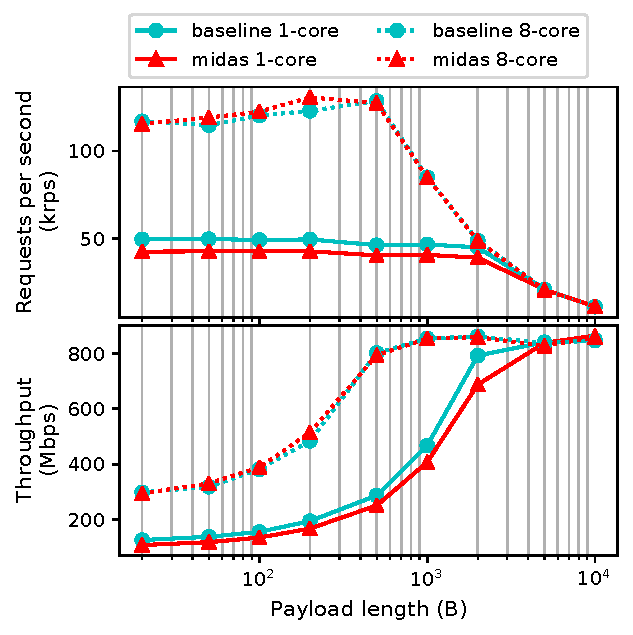
\includegraphics[width=\linewidth]{media/midas/nginx_performance.pdf}
  \caption{Request rates and throughput served by the Nginx server for
          static pages.}
  \label{fig:nginx_perf}
\end{figure}

To better understand \midas' behavior under varying syscall
rates and different core configurations, we study Nginx's (version 1.18)
throughput while varying payload sizes and different worker counts.
Each worker is single threaded and uses one core.
The server is loaded with requests from a separate machine running
a load generater (\Code{bombardier}) with 100 concurrent
connections (chosen to maximize throughput) over a 1Gbps link.
The clients send http requests for files ranging between 20B and
10000B.

In \autoref{fig:nginx_perf}, we plot the request rate and throughput
for Nginx servers running with one and eight workers.
For all configurations, we can see that the rate of requests served
remains almost constant while increasing payload size until the network
link reaches saturation.
Under a saturated network, the request rates for \midas match that
of the baseline system.
With a single worker, \midas' overheads cause a consistent~13--14\%
overhead on the request rate for small packet sizes.
However, we see that \midas has practically no overhead when serving
requests with 8 workers even when packet sizes are too small to
saturate the network link.
In this case, both \midas and the baseline system are limited by the
scalability of the Linux networking stack.

%%%%%%%%%%%%%%%%%%%%
\section{Related Work}
%%%%%%%%%%%%%%%%%%%%

Early work on double-fetch bugs relied primarily on manual
code analysis to identify bugs in kernel code~\cite{YangCSS12, twizsgrakky07ring0}
or in syscall wrappers~\cite{watson2007exploiting}.
Realizing the limited scalability of this approach, particularly
when applied to large codebases such as the Linux kernel, subsequent 
work focussed on automated techniques based on static or dynamic 
analysis techniques, and on leveraging hardware features to mitigate
such bugs.

% Realizing that large projects such as the Linux kernel are not 
% amenable to extensive man
% In this section, we describe the automated tools that followed,
% based on static or dynamic analysis techniques, which can be employed
% to find and mitigate \tocttou bugs.

\paragraph{Static analysis}
%
Static analysis proposals use code analysis to find and fix double fetch
vulnerabilities.
DFTinker~\cite{dftinker} improves the coverage of pattern matching rules
for detecting double fetches in code as initially proposed by Wang~et~al.~\cite{wang2017double}.
Deadline~\cite{deadline} and DFTracker~\cite{wang2019dftracker} further
generalize the analysis by leveraging symbolic execution.

However, static analysis is severely limited by its requirement for
source code, which eliminates possibility of protecting of analyzing
binary-only modules for which code is not available.
In contrast, \midas can also protect such modules since well-behaving
module use the kernel transfer functions to access user memory.
Symbolic execution solves the generality problem of pattern-matching
approaches but has its limitations (path explosion, function pointers,
modelling numerous library functions, etc.).
Deadline~\cite{deadline} specifically requires the additional assumption
that pointer syscall argument do not alias, an assumption that can
wilfully be violated by our adversarial model.

Additionally, the protection allowed by static analysis methods are
limited: only the bugs which are detected can be fixed, and static
analyses are necessarily incomplete.
In contrast, \midas mitigates \emph{all} \tocttou vulnerabilities.
Further, specific cases of double fetches, such as in syscall wrappers
cannot be fixed in code, and require a versioning system such as
\midas in order to enable deep argument inspection.

\paragraph{Dynamic Analysis}
%
Dynamic analysis techniques leverage runtime information and values
to detect double fetches, and are notable in their ability to
find bugs in binaries.

To enable the search for various classes of bugs, Google Project Zero's
Bochspwn project~\cite{jurczyk2013bochspwn} introduced
a comprehensive emulator for \Code{x86} with callbacks to allow
tracing of kernel operations, including memory accesses.
When paired with a syscall fuzzer,
Bochspwn successfully detected and reported double fetches from
these access logs, but suffered from a high rate of false positives.
Another major shortcoming of Bochspwn was its low execution throughput
of 40-80MIPS which limited its ability to explore code paths.
Xenpwn~\cite{wilhelm2016xenpwn} extended Bochspwn's trace-driven 
approach to fuzz hypervisors for double-fetch bugs.
Xenpwn found three double fetches in the Xen hypervisor, but no critical 
vulnerabilities in KVM.

DECAF~\cite{schwartzDECAF} inverts \midas' adversarial model, leveraging
concurrent access to syscall parameters from userspace to detect kernel
accesses via a cache side-channel.
DECAF is strongly reliant on CPU-specific behavior, which
is sensitive to CPU parameters, subject to changes from generation to
generation (or even from core to core) and prone to noise and false sharing.
Following the discovery of transient-execution attacks~\cite{KocherHFGGHHLM019},
proposals such as InvisiSpec~\cite{YanCS0FT19,KhasawnehKSEPA19} have
tried to prevent
information leakage via cache side-channels.
Future generations might entirely close this channel, or introduce constraints
that limits this information flow.

Dynamic analysis techniques can only detect vulnerabilities on executed code
paths, and therefore typically rely on a fuzzer to extensively cover kernel code.
However, fuzzers are inherently incomplete, limiting the ability of dynamic
analysis to find bugs.

% PeriScope\cite{SongH0SNVVKSF19} is out of scope.
% Devices are outside the scope of the current implementation of \midas. Particularly, double fetches from device backed memory is liable to change without any control, but already requires high privileges which the user does not have. DMA accesses to main memory, however, can be protected by the use of IOMMUs with very low overhead [4], and can take advantage of the same \midas mechanisms. [4] Border Control: Sandboxing Accelerators.
% Overall comment: \midas does not seek to overthrow methods that seek to find double fetches, and fix them. In fact, it also allows use as a sanitizer that flags such double fetches. In the meanwhile, however, bugs do persist and are likely to persist in an environment incorporating third-party code in modules and a rapid pace of development. Here, \midas provides a strong, principled guarantee which is also future-proof.

\paragraph{Mitigations}
%
Previous attempts~\cite{schwartzDECAF,dftinker} to eliminate double fetch
vulnerabilities rely on Intel TSX, a hardware transactional
memory implementation, to detect malicious writes to data read by the
kernel.
A defense based on TSX improves upon \midas by reducing the scope for
false sharing from a page size to a cache size.
However, TSX suffers from major limitations which restrict its useability
for general kernel implementations.
Of note, TSX requires that the data working set for the critical section
experiences no L1 cache evictions, even due to contention from a
simultaneously-multithreaded (hyperthreading) core.
Further, TSX is limited to processors from a specific manufacturer (Intel),
leaving the vast majority
of computing devices~(mobile, IoT, AMD processors) unprotected.

%%%%%%%%%%%%%%%%%%%%
\section{Conclusion}
%%%%%%%%%%%%%%%%%%%%

\midas mitigates double-fetch bugs in system calls and protects the operating
system kernel by enforcing the invariant:  \emph{through a syscall's
lifetime, every read to a userspace object will return the same value}.
Our \midas implementation creates on-demand snapshots and copies of pages that
are read and merges any writes through the execution of the system call.
%
Our mitigation protects the core kernel, as well as drivers by carefully
instrumenting functions that interact with the process address space. While our
implementation focuses on Linux for x86-64, our concept is generic and empowers
other kernels to protect themselves against notoriously hard-to-find and
easy-to-exploit double fetch bugs.

The performance evaluation of our prototype implementation is promising.
Compute-bound benchmarks have negligible overhead and even syscall-intensive
benchmarks exhibit low overhead. On one hand, \midas mitigates all double fetch
bugs in the kernel and gives developers a tool to locate such bugs. On the other
hand, \midas sets the foundation for efficient, stateful system call filtering
and validation.
%
We have released the source code of our prototype as open-source at
\url{https://hexhive.epfl.ch/midas/}.

%%%%%%%%%%%%%%%%%%%%%%%%%%%%%%%%%%%%%%%%%%%%%%%%%%%%%%%%%%%%%%%%%%%%%
% SecureCells CORE
%%%%%%%%%%%%%%%%%%%%%%%%%%%%%%%%%%%%%%%%%%%%%%%%%%%%%%%%%%%%%%%%%%%%%
\chapter{SecureCells: A Secure Compartmentalized Architecture}
\label{ch:seccells}
% \epigraph{The real cool stuff was already done.}%
%         {\textit{Me}}

% Copying securecells' paper abstract here
Modern programs are monolithic, combining code of varied provenance without 
isolation, all the while running on network-connected devices. 
A vulnerability in any component may compromise code and data of all other 
components. 
Compartmentalization separates programs into fault domains with limited 
policy-defined permissions, following the principle of least privilege, 
preventing arbitrary interactions between components. 
Unfortunately, existing compartmentalization mechanisms target weak attacker 
models, incur high overheads, or overfit to specific use cases, precluding 
their general adoption. 
The need of the hour is a secure, performant, and flexible mechanism on which 
developers can reliably implement an arsenal of compartmentalized software. 

We present SecureCells, a novel architecture for intra-address space 
compartmentalization. 
SecureCells enforces per-Virtual Memory Area (VMA) permissions for secure and
scalable access control, and introduces new userspace instructions for 
secure and fast compartment switching with hardware-enforced call gates and 
zero-copy permission transfers. 
SecureCells enables novel software mechanisms for call stack maintenance and 
register context isolation. 
In microbenchmarks, SecureCells switches compartments in only 8 cycles on a 
5-stage in-order processor, reducing the switching cost by an order of magnitude
compared to the state-of-the-art. 
Consequently, SecureCells helps secure high-performance software such as an 
in-memory key-value store with negligible overhead of less than $3\%$.
%%%%%%%%%%%%%%%%%%%%%%%%%%%%%%%%
\section{Introduction}
\label{sec:seccells:intro}
%%%%%%%%%%%%%%%%%%%%%%%%%%%%%%%%

% bugs allow access to data/code outside of the current module
Modern software systems are complex but monolithic, 
comprising multiple interacting subsystems,
incorporating third-party code like libraries, plugins, or interpreted code,
while interacting over untrusted 
interfaces including networks, shared memory, file systems, or user input.
The lack of isolation between the components of a monolithic program 
allows vulnerabilities to have far-reaching consequences.
An attacker who exploits one component can corrupt other parts ---
for example, a buggy Linux driver can compromise
core kernel data structures.
The traditional process abstraction for running monolithic software
violates the principle of least privilege~\cite{SaltzerS75}
which requires components to only have access to the data necessary
for their operation.
Instead, all code running within a process' address space has 
equal permissions to all data and code regions
allowing attackers to subvert pre-defined interfaces between components.
For example, calls between components can jump to an arbitrary address
bypassing checks on function call arguments.

% compartmentalization enables least privilege
Intra-address space compartmentalization allows developers to 
\emph{isolate components} of a program within compartments, 
only granting each compartment permissions to access their own data.
When compromised, a buggy component cannot access another
component's data.
Conversely, a component is guaranteed integrity of its private
data against other corrupted compartments.
Compartmentalization is a key defense mechanism that leverages the 
inherent modularity of code to 
fortify the cloud~\cite{v8isolates,ShillakerP20,miller2021} and 
desktop~\cite{fffission} sandboxed environments, 
programs with third-party libraries~\cite{GhosnKPLB21}%,ZimmermannSTP19}, % VasilakisKRDDS18, 
and underpins the design of security-focused microkernel operating
systems~\cite{RozierAABGGHKLLN88, Hildebrand92, LevinCCPW75, GolubDFR90}.
Compartmentalization constrains the negative effects of the myriad possible faults 
in software, 
including memory safety violations and logic errors, 
to compartment boundaries.
For example, the Log4Shell exploit (CVE-2021-44228~\cite{cve202144228}) which
allowed attackers to exfiltrate secrets and inject arbitrary code in
memory-safe programs can be mitigated by isolating the vulnerable Log4j framework
in a separate compartment.

% properties of a good compartmentalization mechanism
The compartmentalization mechanism enforcing
the rules of access and communication between the program's 
components must be secure, performant and flexible.
To be secure, the mechanism must enforce policy-dependent 
restrictions on memory accesses and inter-compartment calls
in the face of powerful attackers.
Particularly, the mechanism must prevent compromised compartments
from escalating their memory access rights or from bypassing
inter-compartment call gates.
%
Developers for performance- and security-critical software such as
operating systems constantly trade off the benefits of protection mechanisms
against their overheads.
The mechanism must implement low overhead checks and operations to support 
fine-grained compartmentalization for such programs.
Faster compartment switching, for example, 
enables developers to refactor programs into smaller compartments
with more frequent compartment switches,
improving security while maintaining the same performance.
%
Finally, a flexible mechanism which is able to support the wide variety of 
desired compartmentalization policies will bolster developer adoption.

% why existing mechanisms are insufficient
Existing compartmentalization mechanisms lack one or more 
desirable features, often trading security for performance,
or flexibility for backward compatibility or implementation simplicity.
Traditional, process-based 
isolation~\cite{KleinEHACDEEKNSTW09,LittonVE0BD16,WitchelCA02MMP}
only permits costly, microsecond-scale compartment switches.
On the other end of the spectrum, protection-key~\cite{guide2011intel} based 
mechanisms~\cite{ParkLXMK19,ERIMOberwagner19,SchrammelWSS0MG20Donky}
are performant, with nanosecond-scale switches,
but fail to deter attackers with code-injection capabilities.
Mechanisms co-locating permissions with page-based virtual 
memory~\cite{ERIMOberwagner19,SchrammelWSS0MG20Donky,LeeSK18,DuHXZC19XPC,
KoningCBGA17,HedayatiGJCSSM19Hodor}
improve compatibility with existing page-tables but
inherit the limited reach of modern 
Translation Lookaside Buffers (TLBs), incurring overheads
for programs with large working sets.
Finally, other mechanisms~\cite{KoningCBGA17,FrassettoJLS18} 
target simpler policies, 
such as protecting a single trusted compartment from an untrusted 
compartment.

\seccells achieves the trifecta of secure, flexible, and high-performance 
compartmentalization by embedding compartmentalization into the 
architectural virtual memory abstraction.
\seccells proposes 
\begin{inparaenum}[\itshape i\upshape)]
\item \emph{TCB-maintained VMA-scale} access control, and 
\item unprivileged (i.e., userspace) instructions implementing 
\emph{securely-bounded} compartmentalization primitives, with
\item software implementing call gates, call stacks, and context isolation.
\end{inparaenum}
Related efforts towards languages, compilers and libraries for
compartmentalization can extend these benefits to developers
by using \seccells as the underlying isolation mechanism.

For the first pillar, access control, \seccells introduces the 
first VMA-granular permissions table consolidating permissions for
all compartments into a single data structure designed for
efficient permission lookups.
In contrast, previous mechanisms use per-compartment permission tables 
with either duplicate VMA bounds information~\cite{WitchelCA02MMP},
duplicate per-page permissions within a 
VMA~\cite{ERIMOberwagner19,SchrammelWSS0MG20Donky},
or both~\cite{DuHXZC19XPC,LittonVE0BD16}.
Deduplicating VMA bounds accelerates compartment switching, eliminating
the need to re-load bounds for the target compartment.
VMA-scale permission tracking requires smaller VMA-based permission
lookaside buffers while also overcoming TLB-reach limits.

For the second pillar, 
\seccells accelerates common compartmentalization operations with
novel, low-cost unprivileged instructions.
Particularly, \seccells is the first mechanism to
allow generic, unprivileged permission transfer from userspace.
\seccells maintains the integrity of permissions by bounding 
the semantics of untrusted userspace operations to known-safe parameters --- 
the hardware checks the compartment switch instruction to enforce call gates,
and permission transfer instructions to prevent privilege escalation.

\seccells' final pillar leverages the flexibility of software for 
operations where possible without compromising security or 
performance (context isolation, call gates and call stack maintenance).
\seccells{} shows the first software mechanism for restoring register context
following a compartment switch, necessary for isolating compartment contexts,
without trusting any general-purpose registers.

In this chapter, we:
\begin{itemize}
  \item define \seccells' key security and performance objectives
        and survey how related mechanisms meet these goals,
  \item propose \seccells, a novel, secure, flexible, and performant 
        mechanism which introduces compartments 
        into the architectural virtual memory abstraction,
  \item apply \seccells to typical application scenarios,
  \item present a hardware implementation of \seccells based on the 
        5-stage in-order RISC-V RocketChip, and
  \item characterize \seccells' performance for compartmentalizing
        micro- and macro-benchmarks.
\end{itemize}

%%%%%%%%%%%%%%%%%%%%%%%%%%%%%%%%
\section{Background}
\label{sec:seccells:background}
%%%%%%%%%%%%%%%%%%%%%%%%%%%%%%%%

Compartmentalization is built on a few basic principles:
modularity, least privilege, and defence in depth.
Compartmentalization mechanisms implement these principles to provide security
to applications through two major properties, isolation of compartments
and controlled communication between compartments.
In these section, we will explain the principles supporting 
compartmentalization and see how these principles lead to security
properties.
The following sections list key objectives for a compartmentalization
mechanism in order to guarantee these security properties.

%-------------------------------
\subsection{Principles supporting compartmentalization}
\label{sec:seccells:background:principles}
%-------------------------------

\paragraph{Abstraction and modularity}
Both software and hardware engineering rely heavily on abstraction, and the
related principle of modularity to manage the every exploding complexity of
computer systems.
Logical parts of systems, for example, are separated into modules, each of 
which hide internal complexity behind well defined interfaces
(commonly called application programming interfaces, or APIs).
One module can use abstract functionality implemented by a separate module
using the module's API without being aware of much of the implementation
complexity.
Modules are typically structured around a specific functionality, and
each module is distributed as a single package.
Common examples of modules include libraries for implementing
cryptographic processing, threading, mathematical operations, compression
and standard language features.
Modularity can also be used to separate instances of the same code running on
logically separate data. 
For example different connections being handled by a server can be separated
into individual modules, as is done by the Apache webserver.
Modularity lends itself to extensibility, allowing the functionality of
applications to be gradually extended beyond its original purpose as more and
more code modules get added.
Modularity has two consequences which greatly benefits compartmentalization
efforts.
First, developers need to develop well-defined interfaces for modules to
enable inter-module communication.
These interfaces can be reused as interfaces if modules are isolated within
compartments.
Second, modules often need to define dependencies or privileges required to 
function.
A compartmentalized system should limit a compartmentalized module's privileges
to those necessary for functioning.

\paragraph{Least privilege}
Least privilege, defined by Saltzer~\cite{SaltzerS75}, states that every
part of a system should operate using the least set of privileges necessary
to perform their function.
This principle aims to control the consequences resulting from a malicious or
buggy module by limiting the potential interactions each module is allowed
to perform.
For example, a media decoding module running on a smartphone application
might be allowed to access the file system to read media files, but should be
denied access to the device's location or to the internet.
Further, an application which downloads media from the internet and plays
it can be split to isolate the two privileges to separate modules.
One module can be allowed to use the internet and save media to a file, and
the second module can be allowed to play media from that file and write to
the device's screen.
A compromised media decoding module, therefore, will be unable to directly
leak information to the internet.
Least privileges also applies to the ability to call functions in
other modules.
For example, a media decoder should be allowed to call functions to open
and read media files, but not to other file system operations like
modifying a file's permissions or owner.
The principle of least privilege should also restrict a module's permissions
to the temporal period where it requires specific privileges.
Privileged programs (like webservers) typically drop elevated privileges 
as soon no longer required, following this principle.

Least privileges require applications to be decomposed into modules 
implementing logically different functionality or working on logically
different data.
Implementing least privilege for modern applications can leverage the
modularity on which systems are already built.

\paragraph{Defence in depth}
Defence in depth poses that systems should not rely on a single layer of
defence, instead using multiple protective measures for the same objective.
Defence in depth mitigates possible shortcomings in a particular defence by
relying on one of the other defences to mitigate attacks.
This principle essentially removes the single point of failure for defences.
For systems software, developers should rely on more than one defence
mechanism to provide stronger security guarantees.
While compartmentalization and memory safety, for example, can both defend
against some memory corruption attacks, each of them can protect against
attacks which the other cannot.
For example, compartmentalization provides no defence against a function
overflowing one of its stack objects into another, which is prevented with
memory safety.
However, memory safety mechanisms might not detect a malicious arbitrary
write from one module to another module's data, but this attack should be
mitigated through compartmentalization.
In general, defence in depth posits that mitigations for memory safety and
compartmentalization complement each other, rather than replacing each other.

%-------------------------------
\subsection{Compartmentalization properties}
\label{sec:seccells:background:properties}
%-------------------------------
A compartmentalized program consists of compartments, each of which is
isolated from other compartments but can communicate through well-defined
APIs.
Isolation and controlled communication aim to limit unintended interactions
between compartments, limiting the damage from such interactions.

\paragraph{Isolation}
Compartmentalization provides isolation between compartments. 
Essentially, each compartment has access permitted to a subset of a system's
resources, including memory, ability to call other compartments, and 
OS resources like files, execution threads or I/O.
Compartments can have private resources, for which no other compartment has
permissions, or resources shared between a subset of compartments.
The compartmentalization mechanism then guarantees that no compartment
without permission can use these resources.
Essentially, a compartment's private resources are isolated from access or
use by other compartments.

With isolation, a compartment is protected from data and control flow attacks
from misbehaving compartments.
With fault isolation or fault handling, an application can also ensure that
faults in one compartment only crash that compartment and not the entire 
application.
Hence, isolation is the first key feature of compartmentalization.

\paragraph{Controlled Communication}
For functionality, compartments require processing by other compartments.
Similar to remote procedure calls, a compartmentalized program requires support
for inter-compartment calls.
Compartments have interfaces, from which other compartments can request 
processing.
A compartment's interface represents the main attack surface for the
compartment, and requires protection.
First, compartments must only be allowed to call authorized compartments.
Second, inter compartment calls must enter the callee at fixed entry points,
allowing call gates to be implemented.
Call gates allow a compartment to ensure the validity of arguments and
switch context, if required, before processing a request.
Therefore, controlled communication is a second key feature of 
compartmentalized programs.

%%%%%%%%%%%%%%%%%%%%%%%%%%%%%%%%
\section{Objectives For Architectural Isolation}
% \section{The case for a novel compartmentalization mechanism}
\label{sec:seccells:reqs}
%%%%%%%%%%%%%%%%%%%%%%%%%%%%%%%%

Compartmentalization mechanisms are characterized by a specific set of 
objectives, which we introduce in this section.
We demonstrate how \seccells' objectives benefit compartmentalization
using two representative programs described below and
discuss how alternate goals lead to the differing designs
of related mechanisms.

The characteristics of a compartmentalization mechanism 
determine its applicability.
Primarily, the mechanism must be \emph{secure} (\req{1}) 
and enforce the
restrictions on data access and communication despite arbitrarily compromised
compartments. 
Second, the mechanism must be \emph{performant} (\req{2}), 
with low overhead for enforcing its checks and restrictions.
A performant mechanism allows high-performance software
to be compartmentalized without violating performance targets.
Finally, a mechanism must be \emph{flexible} (\req{3}) in order to 
support the varying needs of software across security and 
performance criticality, and their corresponding isolation policies.
A flexible mechanism does not make additional assumptions such as
a hierarchical trust structure among compartments, and allows
data to be shared in an arbitrary fashion.
We concretize these objectives, based on insights from existing
and candidate compartmentalized programs and related work, 
in the following subsections.
We justify each objectives' importance using the
two characteristic programs described below.

\begin{figure}
  \centering
  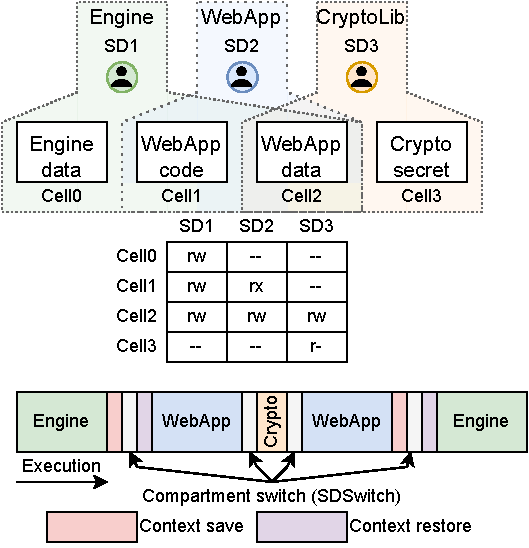
\includegraphics[width=0.65\linewidth]{media/seccells/browser_webapp.pdf}
  \caption{Browser compartmentalization with three compartments.}
  \label{fig:seccells:browser_eg}
  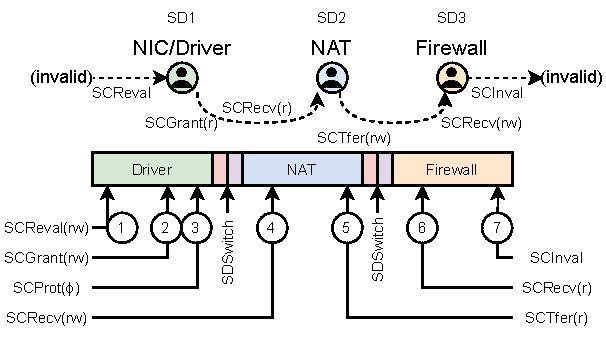
\includegraphics[width=\linewidth]{media/seccells/dataflow_app.pdf}
  \caption[Permission transfers for a packet between \seccells compartments.]
          {Permission transfers for a packet between \seccells compartments. 
            The figure shows the compartment executing the relevant \seccells 
            instructions on one core.}
  \label{fig:seccells:dataflow_app}
  %\Description[<short description>]{<long description>}
\end{figure}

\paragraph{Use case: Browser}
The first program, a browser (\autoref{fig:seccells:browser_eg}), consists of
a just-in-time (JIT) compilation engine (Engine), 
a sandboxed web application (WebApp) compiled and executed by the Engine, and 
a cryptographic library (CryptoLib) storing a secret key for encryption.
The compartmentalization policy aims to isolate the Engine's data
and CryptoLib's secret from the possibly malicious WebApp.
Borrowing the threat model for browsers, we assume that the 
WebApp can exploit bugs in the Engine's compiler to 
generate and execute arbitrary code as the WebApp compartment,
ultimately aiming to leak the browser's data or the cryptographic secret.
The developer aims to prevent unauthorized inter-compartment data accesses
by enforcing the per-compartment permissions shown in the figure.
To maintain similar performance to the monolithic version, the developer
desires minimal overhead from operations added due to compartmentalization:
context switching and compartment switching.

\paragraph{Use case: Network Function Virtualization}
The second program is a virtual network function pipeline 
(\autoref{fig:seccells:dataflow_app}) consisting of three stages progressively
performing processing steps on a stream of packets.
In particular, this pipeline has three compartmentalized stages, 
implementing the network card driver (Driver) which
generates packets, 
a network address translation (NAT) stage which translates IP 
addresses in the header based on a translation table, and
a firewall stage that implements checks on the packet headers
based on a rule table.
In this example, we omit further stages for simplicity.
Middleboxes in datacenters and the internet~\cite{MartinsAROHBH14}
commonly contain virtual network functions sharing a buffer pool
in uncompartmentalized dataflow pipelines.
Translation and rule tables in the NAT and Firewall compartments
must be isolated in private regions, protecting them from potential bugs 
in the Driver compartment that processes input from untrusted traffic 
from external sources.
The programmer requires isolation of network stages for high reliability
of the middlebox and low cost for passing packets between stages for 
line-rate packet processing, enabled by zero-copy packet flow 
through permission transfer.


%-------------------------------
\subsection{Threat Model}
\label{sec:seccells:reqs:threat}
%-------------------------------

Our threat model assumes an attacker who wants to compromise a 
compartmentalized program with multiple communicating compartments.
We assume that the attacker has compromised one or more compartments, and
gained the ability to both generate arbitrary code and execute it,
but is restricted to the compromised compartments.
The attacker wishes to compromise confidentiality, integrity, or 
gain code execution in other compartments.
%
For example, the attacker might try to:
% \begin{inparaitem} for an inlined bullet point list instead
\begin{itemize}
  \item gain permissions and directly access (load/store) 
        another compartment's private memory,
  \item inject unsolicited code/data regions in another 
        compartment's memory,
  \item execute unintended code in another compartment,
  \item create new compartments, or
  \item achieve any combination of the above.
\end{itemize}

The policy used for compartmentalization is assumed to be sound, and the software
implementations of the modules comprising compartments are assumed to be
free of bugs that can be exploited via only their exposed communication
interfaces.
\seccells' trusted computing base (TCB) consists of the hardware implementation
and the supervisor.
Exploitable bugs in the policy or TCB can lead to a compromise irrespective of the
compartmentalization mechanism.
While speculative side-channel attacks are outside the scope of our threat model,
we discuss \seccells' speculative resiliency in \autoref{sec:seccells:discussion}.

%-------------------------------
\subsection{Security Objectives}
\label{sec:seccells:reqs:security}
%-------------------------------
A secure mechanism must enforce restrictions on a compartmentalized program,
as described below.

\paragraph{Obj. \req{1a}}
Mechanisms must implement \emph{access control},
validating every memory access against the policy.
For the browser in \autoref{fig:seccells:browser_eg}, the table
holds policy-defined permissions for each compartment and memory region.
Mechanisms must, for example, prevent all accesses by the compromised
WebApp from reading the Engine or CryptoLib's private regions as per the
policy.
Mechanisms must also prevent corruption of policy-defined permissions
stored in memory or registers.
Intel MPK-based protection~\cite{ParkLXMK19}, for example, loads
permissions from a user-controlled register when executing a
\Code{wrpkru} instruction, allowing a compartment to corrupt its 
own permissions.

\paragraph{Obj. \req{1b}}
Inter-compartment communication consisting of cross-compartment calls 
demand \emph{validity checks}.
Relevant validity checks include checking that 
\begin{inparaenum}[\itshape i\upshape)]
  \item the entry point is valid,
  \item the calling compartment is allowed to call the target compartment, 
  \item the return respects the call stack, and
  \item the passed arguments are valid.
\end{inparaenum}
Compartment switches from the WebApp to the Engine must use valid entry
points which are followed by argument-validating code. Failure to enforce this
constraint enables
control-flow attacks such as return-oriented programming (ROP).
Vanilla Intel MPK-based protection also lacks such entry-point checks
to accompany \Code{wrpkru} instructions.

\paragraph{Obj. \req{1c}}
\emph{Context isolation} accompanying a cross-compartment call is 
essential for protecting mutually distrusting compartments.
After a cross-compartment call, the callee compartment (for example, the Engine) 
must be able to fetch its context without trusting the registers which
are controlled by the caller (correspondingly, the WebApp), 
representing an attack vector.
The WebApp, for example, could try to switch to the Engine with a malicious stack pointer
register, attempting to corrupt the Engine by reading from the wrong stack.
CODOM~\cite{VilanovaBNEV14}, for example, assumes a migrating thread model
and is vulnerable to attacks through an invalid register state.

\paragraph{Obj. \req{1d}}
Mechanisms that allow untrusted compartments to modify or transfer their 
permissions must prevent privilege escalation %~\cite{ZeldovichBKM06} 
through \emph{TCB-imposed limitations} on these operations.
Specifically, compartments should only be allowed to surrender access 
permissions or transfer existing permissions to other compartments.
A stage in the network function pipeline, for example, should not be allowed
to grant write permissions for a packet to the next stage if it has
read-only permissions.
Transferring permissions between compartments must also be mutual, requiring
explicit actions from both compartments.
One-directional permission transfers studied by 
Lipton~\textit{et. al.}~\cite{LiptonS77} 
allow compartments to either steal other compartments'
permissions (violating confidentiality) or
inject illegal data or code into other compartments (violating integrity).
Linux, which allows processes to specify their own permissions
when \Code{mmap}ing shared regions, violates this objective without 
syscall mechanisms like SECCOMP.

\paragraph{Obj. \req{1e}} 
\emph{Temporary exclusive access} to otherwise 
shared data regions enables compartments to use data regions safely,
preventing exploitation of double-fetches.
With exclusive access to a packet, the Firewall stage of the network function
pipeline can safely validate and use addresses in the packet header in-place 
(without copying), with the assurance that another corrupt stage cannot
concurrently modify the packet.
XPC~\cite{DuHXZC19XPC} recognizes this objective, allowing exclusive access
to a single region tracked by the Relay Segment register.

\paragraph{Obj. \req{1f}} 
\emph{Auditability}, the ability to easily determine the 
global access permissions, facilitates auditing compliance to a 
compartmentalization policy by checking which compartments have access to
which memory region.
A browser might regularly audit its permissions to ensure that the WebApp
has not escalated its privileges.
An audit for a mechanism with a centralized permissions store, 
such as page tables, must only check this store simplifying audits.
In contrast, an audit for CHERI~\cite{WatsonWNMACDDGL15} requires an 
expensive, full-memory scan since the set of memory regions accessible to a
compartment is the transitive closure of capabilities held in its registers,
along with capabilities held in any memory region accessible through these 
registers.

%-------------------------------
\subsection{Performance Objectives}
\label{sec:seccells:reqs:performance}
%-------------------------------
Low-overhead checks and operations allow performance-critical
programs to be compartmentalized.

\paragraph{Obj. \req{2a}} 
\emph{Single-cycle access verification} in the common case
is essential for core throughput.
While most mechanisms meet this objective in the best (not common) case, 
page-table based isolation mechanisms suffer from the limited scalability
of Translation Lookaside Buffers (TLBs) used to cache permissions.
Programs with large datasets can incur high TLB miss rates, with 
correspondingly high verification latency in the common case due to 
page-table walks.
UNIX process-based protection particularly suffers from this limitation since
modern Address Space ID (ASID)-tagged TLBs will effectively contain duplicate
entries for a shared page with separate permission for each compartment,
effectively dividing an already capacity-limited structure among 
compartments~\cite{HsuHEP16}.
This objective implicitly requires the mechanism to support
a sufficiently large number of compartments and data regions.
A mechanism with small limits, like Intel MPK which is restricted to
16 colors for data regions, will incur overheads from software workarounds
required to virtualize the corresponding resource~\cite{ParkLXMK19}.

\paragraph{Obj. \req{2b}} 
Cross-compartment calls are essential and
frequent for communication between fine-grained compartments
necessitating \emph{fast compartment switches}.
Fine-grained library isolation~\cite{GhosnKPLB21} requires compartment 
switches accompanying every function call to an untrusted library.
A program isolating short-running functions, 
such as AES encryption using hardware AES-NI extensions, 
can incur a compartment switch every tens or hundreds of 
cycles~\cite{AbdAllahAES}.
Specialized hardware instructions accessible from userspace are
essential for cheap compartment switches in tens of cycles.
Even the fastest supervisor-mediated compartment switch still costs
hundreds of cycles~\cite{WatsonWNMACDDGL15}.

\paragraph{Obj. \req{2c}}
\emph{Fast, zero-copy permission transfer} enables programs to 
efficiently move data between compartments.
Data copying for passing large buffers during 
compartment calls can overwhelm high-performance programs, 
such as our example network function pipeline.
Such applications typically pass packets by reference between 
unisolated stages profiting from zero-copy.
Cheap permission transfers, within ten to hundred cycles, enable 
such applications to be compartmentalized with performance
comparable to the monolithic versions.
UNIX process-based permission transfers instead involve microsecond-scale
system calls, precluding their use for practical compartmentalization.

%-------------------------------
\subsection{Flexibility}
\label{sec:seccells:reqs:flexibility}
%-------------------------------

A mechanism demands flexibility to be suitable
to compartmentalization across a variety of application domains. 

\paragraph{Obj. \req{3a}}
For flexibility, a mechanism must support \emph{arbitrary sharing of data
regions},
requiring independent per-compartment per-region permissions.
A private region, for example, should be accessible by only a single
compartment.
Another shared region might allow read access to one compartment, 
write access to another, and execute permissions to a third.
Mechanisms that target hierarchical security, for example, limit
flexibility --- the trusted  compartment implicitly has permission
to access an untrusted compartment's data --- and exclude wide 
applicability.
In contrast, even if the WebApp in the browser trusts the Engine,
the Engine is denied execute permissions to the WebApp's code.
A mechanism must support, but not be exclusive to, specific trust
models such as nested compartments.

\paragraph{Obj. \req{3b}}
To scale performance overheads with security objectives, we
introduce a desirable property, \emph{security-proportionality}.
A security-proportional mechanism allows policies to trade-off 
overheads for security when unnecessary.
Despite not trusting the WebApp, transitions from the WebApp to
CryptoLib can elide context switching required for register 
isolation under a specific condition.
Verification approaches~\cite{KolosickNJWLGJS22Verizero,ChenRSL16} 
can be used to prove that a small function in CryptoLib does not leak the key
under the assumption that entry points are enforced,
and that the function's code overwrites registers used to store the key 
before returning to the WebApp.
By using the cheaper migrating thread model~\cite{FordL94},
a security-proportional mechanism can reduce overheads where acceptable.
Process-based isolation, for example, is not security-proportional
since every compartment switch incurs the same non-negotiable overheads 
(including context switching, page-table switching, or scheduling).

%-------------------------------
\subsection{Alternate Visions for Compartmentalization}
\label{sec:seccells:reqs:related}
%-------------------------------

% Text for the camera ready. Reinstate.
\seccells envisions a future where the mechanism supports 
widespread application
compartmentalization efforts, with consequently differing goals
and designs compared to related mechanisms.
% \seccells targets different goals compared to related mechanisms
% consequently resulting in drastically differing designs.
% 
First, some mechanisms only support \emph{custom-tailored use cases}
such as differentiating between single trusted-untrusted 
compartments~\cite{HedayatiGJCSSM19Hodor,KoningCBGA17,Kilpatrick03}, % ,MogosanuRD18
or a binary classification of data as (in)sensitive~\cite{FrassettoJLS18}.
CODOMs~\cite{VilanovaBNEV14} link code addresses to compartments,
restricting code sharing that is abundant in modern programming.
Specialization allows simpler hardware mechanisms, but do not support
a broad spectrum of applications.
Second, \seccells does not aim to compartmentalize existing software with
zero-modifications.
While automated isolation techniques provide a crucial first step towards
compartmentalized programs~\cite{RoesslerAPMPKPB21,KirthDCLDGNVF22,
VasilakisKRDDS17}, security-critical software requires refactoring to fully
realize the benefits of proper compartmentalization.
Finally, related works target \emph{compatibility with legacy hardware}
or existing or upcoming software/hardware mechanisms and abstractions for 
isolation.
Numerous mechanisms try to compartmentalize using process-based isolation
implemented by the OS~\cite{LittonVE0BD16,DuHXZC19XPC,KleinEHACDEEKNSTW09}, 
retrofitting compartmentalization onto an abstraction originally designed for
multiprogramming on unicore processors.
Others leverage Intel MPK~\cite{HedayatiGJCSSM19Hodor,ERIMOberwagner19,KoningCBGA17}
or similar protection-key based mechanisms~\cite{SchrammelWSS0MG20Donky},
synergizing with traditional page table-based virtual memory.
Targeting immediate adoption, Hodor~\cite{HedayatiGJCSSM19Hodor} and 
LOTRx86~\cite{LeeSK18} (ab)used existing processor features intended for 
other purposes to isolate compartments.
HAKC~\cite{mckee2022preventing} leverages state-of-the-art ARM extensions, 
PAC and MTE, to compartmentalize the Linux kernel, but requires a two-level 
clustering of closely-connected compartments to overcome MTE's 
compartment scaling limitations and still incurs a significant performance hit.
With the sole exception of Mondrian~\cite{WitchelCA02MMP}, proposals
assume current page-based virtual memory.
Meanwhile, trends in applications and memory architectures have led to a 
resurgence in range-based translations and protections among academic 
proposals~\cite{BasuGCHS13,YanLNB19,PhamVJB12,0003BOBFP21midgard,KarakostasGACHM15}
and commercial processors including AMD's Zen lineup~\cite{preservingvma}.
\autoref{tab:seccells:req_comparison} summarizes the objectives satisfied by related 
mechanisms (justification in Appendix~\ref{app:seccells:justification_table1}).
We discuss related mechanisms further in \autoref{sec:seccells:related}.
 
% Camera ready TODO: Should I make figure and table styles consistent?
% If yes, follow the procedure described here
% https://tex.stackexchange.com/questions/166814/table-caption-in-uppercase-i-dont-know-why
\begin{table}
  \centering
  \caption[Qualitative comparison of compartmentalization mechanisms]
          {Comparison of compartmentalization mechanisms based on 
          compliance with the objectives described in \autoref{sec:seccells:reqs}.
          Limited compliance is marked with ``$\sim$''.
          }
% \begin{tabular}{l | c c c c c c | c c c | c c |}
  \begin{tabular}{l | c@{\hspace{1em}} c@{\hspace{1em}} c@{\hspace{1em}} c@{\hspace{1em}} c@{\hspace{1em}} c@{\hspace{1em}} | c@{\hspace{1em}} c@{\hspace{1em}} c@{\hspace{1em}} | c@{\hspace{1em}} c@{\hspace{1em}} |}
    \toprule
              & \multicolumn{6}{c|}{\req{1}}                  & \multicolumn{3}{c|}{\req{2}} & \multicolumn{2}{c|}{\req{3}} \\
              & a     & b     & c     & d     & e     & f     & a     & b     & c     & a     & b             \\ \midrule
  UNIX        & \yes  & \yes  & \yes  & N/A   &       & \yes  &       &       &       & \yes  &               \\
  Mondrian    & \yes  & \yes  & \yes  & N/A   &       & \yes  & \yes  &       &       & \yes  &               \\
  lwC         & \yes  & \yes  & \yes  & N/A   &       & \yes  &       &       &       & \yes  &               \\
  CODOM       & \yes  & \yes  &       & N/A   &       & \yes  &       & \yes  &       &       & \yes          \\
  XPC         & \yes  & \yes  & \yes  & \yes  & \yes  & \yes  &       & \yes  & $\sim$& \yes  &               \\
  MPK         &       &       &       &       &       & $\sim$&       & \yes  & \yes  & \yes  & \yes          \\
  ERIM        & $\sim$& $\sim$&       &       &       & $\sim$&       & \yes  & \yes  & \yes  & \yes          \\
  Donky       & $\sim$& \yes  &       & N/A   &       & \yes  &       & \yes  & \yes  & \yes  &               \\
  CHERI       & \yes  & \yes  & \yes  &       &       &       &       &       & \yes  & \yes  &               \\
  \seccells   & \yes  & \yes  & \yes  & \yes  & \yes  & \yes  & \yes  & \yes  & \yes  & \yes  & \yes          \\ \bottomrule
  \end{tabular}
  \label{tab:seccells:req_comparison}
\end{table}

\paragraph{Complementary requirements}
To satisfy application requirements,
programs compartmentalized with \seccells' mechanisms require
complementary properties from other parts of the system
including secure compartmentalization policies, 
a secure and performant supervisor interface, 
and formal verification of application-level properties
aided by programming conventions.
For example, supervisors might include a syscall for 
microsecond-scale compartment creation~\cite{LittonVE0BD16}.
Safe calling conventions can provide formal guarantees against
inadvertent information leakage from the stack~\cite{SkorstengaardDB20}.
These investigations are outside the scope of this thesis.

\paragraph{\seccells overview}
\seccells is a compartmentalization mechanism designed
to satisfy the above objectives across a wide array of 
programs, providing flexibility and performance without compromising on 
security.
\seccells stores permissions in a centralized permissions table accessible 
only by the supervisor and hardware.
A novel, range-based memory management unit (MMU) and 
lookaside buffer design (\autoref{sec:seccells:design:access_ctl})
allows single-cycle access control on the fast path satisfying 
objectives \req{1a}, \req{1f}, \req{2a}, and \req{3a}.
\seccells introduces fast, userspace instructions for common 
compartmentalization operations (see \autoref{tab:seccells:seccell_ops}): 
switching compartments, transferring permissions and validating
exclusive access for data regions (\autoref{sec:seccells:design:instructions}).
These instructions satisfy requirements \req{1b}, \req{1e},
\req{2b}, \req{2c}.
\seccells delegates context isolation, call-stack maintenance,
and argument validation to software.
\autoref{sec:seccells:design:softmech} outlines how software can
securely and efficiently implement context isolation and call-stack 
maintenance.
Software implementing these functions satisfy security (\req{1b}, \req{1c})
and flexibility (\req{3a}, \req{3b}) objectives.

%%%%%%%%%%%%%%%%%%%%%%%%%%%%%%%%
\section{\seccells}
\label{sec:seccells:design}
%%%%%%%%%%%%%%%%%%%%%%%%%%%%%%%%

\begin{figure}
  \centering
  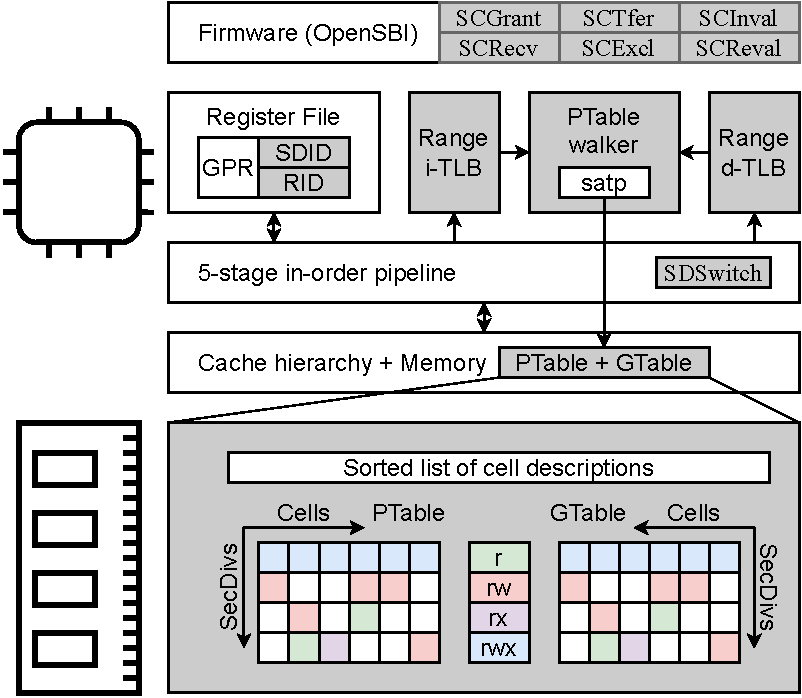
\includegraphics[width=0.85\linewidth]{media/seccells/seccell_arch.pdf}
  \caption[\seccells: Architecture.]
          {\seccells' architecture, highlighting modified hw/sw in gray.}
  \label{fig:seccells:seccell_arch}
  %\Description[<short description>]{<long description>}
\end{figure}

\seccells proposes hardware-software co-design to satisfy the
manifold objectives for efficient and secure compartmentalization.
The key insight that \emph{compartmentalization operations from untrusted userspace
are secure with TCB-maintained permission checks} allows \seccells to
implement compartment switch and permission transfer through
trusted hardware-checked userspace instructions which are
hundred to thousand times faster compared to traditional supervisor calls.
Pragmatically, \seccells retains software for operations such as 
context switching which, while common, would not benefit significantly 
from hardware support.
Software implementations of such operations achieve higher flexibility and
resilience to implementation errors at negligible or low additional performance
cost compared to a hardware implementation.
% Hardware compartment switching eliminates generic supervisor-dependent 
% overheads due to system call dispatch, scheduling and resource accounting, 
% as well as an extra context switch and pipeline serialization for entering
% the kernel.
For example, both hardware and software context switching can saturate
the L1 data cache bandwidth, achieving similar performance.
The second insight is that VMA-based permission tracking eliminates 
permission duplication inherent in page-table entries for pages 
within a VMA.
\seccells leverages this insight, eliminating overheads for 
permission storage (compared to equivalent page tables) and 
allowing hundred-times smaller core-side lookaside buffers. 

\seccells protects compartments, application-defined mutually untrusting
parts of a program, by controlling their access to memory regions.
Each compartment is allocated a Security Division (\secdiv)
with individual permissions to each VMA-granularity data region (\cell{}).
The Browser (\autoref{fig:seccells:browser_eg}), for example, has 
three compartments (Engine, WebApp and CryptoLib) allocated 
\secdivx{1}-\secdivx{3}, and four \cell{}s.
\seccells augments each core with a read-only register (\sid) tracking 
the currently executing compartment.
Along with a table for storing permissions (\ptable) and a modified
MMU for enforcing the permissions, \seccells implements single-cycle
access control.
The WebApp \secdiv has executable permissions
to one code \cell and read-write permission to one data \cell.
Userspace instructions (see \autoref{tab:seccells:seccell_ops}) enable 
secure compartment switching and permission surrender/transfer.
% For implementation reasons regarding how risc-v wants to use ecalls to enter
% the kernel, we must make urid writable by the kernel in our prototype.
% In a pure seccells world, where sdswitches are used for syscalls, we
% might no longer need writable urid (caveat switching programs).
%
% Mat: we could argue that privileged world can always write/override but this
% may be too implementation specific
Another per-core read-only register (\rid) tracks the caller after a 
compartment switch, allowing the callee to securely identify 
its caller.
% \andres{Not sure if this argument is enough, we can use a memory
% segment for that and rely on a compartmentalization policy (memory segment not
% writable by the callee). Is the performance argument sufficient?}
% Atri: Not sure how that would work
During permissions transfer, a granted permissions table (\gtable) tracks
outstanding permissions.
Further, the design implements context isolation and secure call stacks
in software leveraging the above hardware primitives.
\autoref{fig:seccells:seccell_arch} summarizes \seccells's architecture.
The detailed layout of cell descriptors, the \ptable, and the \gtable 
are shown in Appendix~\ref{app:seccells:ptable}.


%-------------------------------
\subsection{Access control}
\label{sec:seccells:design:access_ctl}
%-------------------------------
The Permissions Table (\ptable) stores 
per-cell, per-\secdiv permissions for the compartmentalized 
program.
For each \cell, the permissions for each \secdiv are independent
and define the degree of sharing for that \cell.
Compartment-private data stores allow only one \secdiv non-null 
permissions in this table.
Shared \cell{}s can be readable, writable, or executable by more than one
\secdiv.
For a JIT compiler, the \cell holding generated data will be writable
by the compiler \secdiv, while being executable by the sandboxed code's
\secdiv.
The \ptable is stored in privileged supervisor memory, restricting
accesses (including stores) from userspace.
\autoref{fig:seccells:browser_eg} shows the permissions for the three browser 
compartments, assigned to separate \secdiv{}s, to the four 
data regions, similarly assigned to \cell{}s.
\seccells' current \ptable design supports a large number of 
\secdiv{}s and \cell{}s ($2^{29}$ and $2^{32}$ respectively), 
vastly exceeding application requirements.
A finely-compartmentalized modern browser, for example, will only require
a few hundred compartments, isolating each loaded shared 
library (around 100 on the author's Firefox installation)
and per-tab rendering compartments~\cite{barth2008security}.

\seccells replaces the core's MMU with a \ptable walker and 
range-based lookaside buffers for permissions and translations.
The MMU checks access permissions based on the accessed address and
the executing \secdiv identified by the core's \sid register.
The lookaside buffers track a small number of frequently accessed
\cell{}s, along with \sid-tagged permissions.
In the common case, access control verifies permissions from
entries in this buffer.
When accesses miss in this buffer, the \ptable walker reads the
required permission from the \ptable.
The walker first performs a (fast) binary search in a sorted list of permissions
to find the correct cell containing the accessed address, then
reads the correct permission from the \ptable for that cell.
The location of the permission in the \ptable is found through very 
simple arithmetic.

\seccells' \ptable layout and MMU design has three
key advantages: fast \ptable walks, scalability to large data 
working sets, and low silicon cost.
The \ptable layout aids fast permission lookups by
sorting the \cell descriptors, allowing a binary search
for the \cell descriptor containing an address, 
and the contiguous layout of the permissions for a particular
\secdiv, which improves spatial locality for \ptable walks.
Range-based lookaside buffers also enable scalability for
programs with large datasets, since permissions should be 
verified against TLB entries in the common case.
With growing dataset sizes, traditional processors require larger 
TLBs in order to track additional page translations and permissions.
Importantly, all permissions for pages within a VMA are
the same, leading to duplication in TLB entries' permissions.
However, the growth of program datasets has exceeded the
TLB reach of modern processors, leading to attempts at 
range-based translations (explicitly managed by the 
supervisor~\cite{YanLNB19}, or implicitly through 
coalescing~\cite{PhamVJB12}).
In contrast, as dataset sizes grow, the \cell count remains 
constant and the size of \cell{}s increases.
Previous work in range-based translation caching~\cite{YanLNB19,0003BOBFP21midgard} 
have also demonstrated that 
processors require hundred-times smaller range-based lookaside buffers 
than in traditional systems, drastically reducing silicon cost.
Research proposals~\cite{0003BOBFP21midgard, ZhangSRL10} 
have also tackled
external fragmentation from range-based translations 
by introducing a system-wide page table after the
last-level cache.

%-------------------------------
\subsection{Userspace Instructions}
\label{sec:seccells:design:instructions}
%-------------------------------

\begin{table}[]
  \centering
  \caption{Overview of \seccells' userspace instructions.}
  \begin{tabular}{l | l}
    \toprule
    Instruction & Purpose                                           \\
    \midrule
    \sdswitch   & Switch to another \secdiv                         \\
    \scprot     & Change current \secdiv{}'s permission to \cell    \\
    \scinval    & Mark a \cell invalid                              \\
    \screval    & Revalidate an invalid \cell                       \\
    \scgrant    & Grant \cell permissions to another \secdiv        \\
    \screcv     & Accept granted \cell permissions                  \\
    \sctfer     & Grant and drop \cell permissions                  \\
    \scexcl     & Check for exclusive access to a \cell             \\
    \bottomrule
  \end{tabular}
  \label{tab:seccells:seccell_ops}
\end{table}

\begin{figure*}[!t]
  \vspace{-1\baselineskip}
  \rule{\textwidth}{1pt}
  \centering
  \textbf{\seccells Program State\\}
  \vspace{-0.5\baselineskip}
  \rule{\textwidth}{1pt}
  \vspace{-2\baselineskip}
  \begin{multicols}{2}
    \begin{algorithmic}[1]
      \State $S$ = Set of $M$ \secdiv{}s incl. supervisor $SD_{sup}$
      \State $C$ = Set of $N$ cells, each valid or invalid
      \State Per-core register $SID$
      \State Per-core register $RID$
      \State \ptable $PT: S \times C \mapsto \mathscr{P}(\set{r, w, x})$
      \State \gtable $GT: S \times C \mapsto S \times \mathscr{P}(\set{r, w, x})$
    \end{algorithmic}
  \end{multicols}
  \vspace{-1.4\baselineskip}
  \rule{\textwidth}{1pt}

\vspace{-0.7\baselineskip}
\begin{multicols}{2}
\removelatexerror

    % General notation:
    % c_i         for a cell
    % SD_j        for a secdiv
    % p_{i,j}     for PT(SDj,ci)
    % gp_{tgt}    for GT perms

    % SDSwitch algorithm
    \begin{algorithm}[H]
      \caption{SDSwitch($addr$, $SD_{tgt}$) \\
        Switch to $SD_{tgt}$ at instruction pointer $addr$   }
        \begin{algorithmic}[1]

          \State $c_i \gets cell(addr)$
          \State \textbf{assert} $valid(c_i)$

          \State \textbf{assert} instruction at $addr$ is $SDEntry$
          \State \textbf{assert} $x \in PT(SD_{tgt}, c_i)$
          \State instruction pointer $\gets addr$
          \State $RID \gets SID$
          \State $SID \gets SD_{tgt}$
        \end{algorithmic}
        \label{alg:sdswitch}
    \end{algorithm}
    \vspace{-0.5\baselineskip}

    % SCProtect algorithm
    \begin{algorithm}[H]
      \caption{SCProt($addr$, $perm$) \\
      Restrict rights to $addr$ to $perm$              }
      \begin{algorithmic}[1]

        \State $c_i \gets cell(addr)$
        \State \textbf{assert} $valid(c_i)$

        \State $p_{i,cur} \gets PT(SD_{cur}, c_i) $
        \State \textbf{assert} $perm \subseteq p_{i,cur}$

        \State $PT(SD_{cur}, c_i) \gets perm$
      \end{algorithmic}
      \label{alg:scprotect}
    \end{algorithm}
    \vspace{-0.5\baselineskip}

    % SCGrant algorithm
    \begin{algorithm}[H]
      \caption{SCGrant($addr$, $SD_{tgt}$, $perm$) \\
      Grant $SD_{tgt}$ $perm$ rights to $addr$             }
      \begin{algorithmic}[1]

        \State $c_i \gets cell(addr)$
        \State \textbf{assert} $valid(c_i) \land perm \ne \phi$

        \State $p_{i,cur} \gets PT(SD_{cur}, c_i)$
        \State \textbf{assert} $perm \subseteq p_{i,cur}$

        \State $GT(SD_{cur}, c_i) \gets (SD_{tgt}, p_{tgt})$
      \end{algorithmic}
      \label{alg:scgrant}
    \end{algorithm}
    \vspace{-0.5\baselineskip}

    % SCRecv algorithm
    \begin{algorithm}[H]
      \caption{SCRecv($addr$, $SD_{src}$, $perm$) \\
      Accept $perm$ rights to $addr$ from $SD_{src}$      }
      \begin{algorithmic}[1]

        \State $c_i \gets cell(addr)$
        \State \textbf{assert} $valid(c_i) \land perm \ne \phi$

        \State $(SD_{tgt}, gp_{tgt}) \gets GT(SD_{src}, c_i)$
        \State $p_{i,cur} \gets PT(SD_{cur}, c_i)$
        \State \textbf{assert} $SD_{cur} = SD_{tgt} \land perm \subseteq gp_{tgt}$

        \If{$perm = gp_{tgt}$}
          \State $GT(SD_{src}, c_i) \gets (SD_{inv}, \phi)$
        \Else
          \State $GT(SD_{src}, c_i) \gets (SD_{tgt}, gp_{tgt} - perm)$
        \EndIf
        \State $PT(SD_{cur}, c_i) \gets perm \cup p_{i, cur} $

      \end{algorithmic}
      \label{alg:screcv}
    \end{algorithm}
    \vspace{-\baselineskip}

    % SCTfer algorithm
    \begin{algorithm}[H]
      \caption{SCTfer ($addr$, $SD_{tgt}$, $perm$) \\
      Transfer all $perm$ rights for $addr$ to $SD_{tgt}$    }
      \begin{algorithmic}[1]
        \State SCGrant($addr$, $SD_{tgt}$, $perm$)
        \State SCProtect ($addr$, $\phi$)
      \end{algorithmic}
      \label{alg:tfer}
    \end{algorithm}
    \vspace{-1.5\baselineskip}

    % SCReval algorithm
    \begin{algorithm}[H]
      \caption{SCReval($addr$, $perm$)  \\
      Re-validate address $addr$ with $perm$ rights}
      \begin{algorithmic}[1]

        \State $c_i \gets cell(addr)$
        \State \textbf{assert} $invalid(c_i) \land perm \ne \phi$

        \State Validate $c_i$
        \State $PT(SD_{cur}, c_i) \gets perm$

      \end{algorithmic}
      \label{alg:screval}
    \end{algorithm}
    \vspace{-1.5\baselineskip}

    % SCInval algorithm
    \begin{algorithm}[H]
      \caption{SCInval($addr$)  \\
      Invalidate $addr$ cell}
      \begin{algorithmic}[1]

        \State $c_i \gets cell(addr)$
        \State \textbf{assert} $valid(c_i)$

        \ForAll{$SD_j \in S - \set{SD_{sup}, SD_{cur}}$}
          \State $p_{i, j} \gets PT(SD_j, c_i)$
          \State $(SD_{tgt}, gp_{tgt}) \gets GT(SD_j, c_i)$
          \State \textbf{assert} $p_{i,j} = \phi \land gp_{tgt} = \phi \land SD_{tgt} = SD_{inv}$
        \EndFor

        \State $PT(SD_{src}, c_i) \gets \phi$
        \State $GT(SD_{cur}, c_i) \gets (SD_{inv}, \phi)$

        \State Invalidate $c_i$
      \end{algorithmic}
      \label{alg:scinval}
    \end{algorithm}
    \vspace{-1.5\baselineskip}

    % SCExcl algorithm
    \begin{algorithm}[H]
      \caption{SCExcl($addr$, $perm$) \\
      Verify exclusive $perm$ rights to $addr$       }
      \begin{algorithmic}[1]

        \State $c_i \gets cell(addr)$
        \State \textbf{assert} $valid(c_i) \land perm \ne \phi$

        \State $p_{i,cur} \gets PT(SD_{cur}, c_i) $
        \State \textbf{assert} $perm \subseteq p_{i,cur}$

        \State $ (SD_{tgt}, gp_{tgt}) \gets GT(SD_{cur}, c_i)$
        \If{$ perm \cap gp_{tgt} \neq \phi$}
          \State \textbf{return} $False$
        \EndIf

        \State $excl \gets True$
        \ForAll{$SD_j \in S - \set{SD_{sup}, SD_{cur}}$}
          \State $p_{i,j} \gets PT(SD_j, c_i)$
          \State $(SD_{tgt}, gp_{tgt}) \gets GT(SD_j, c_i)$
          \If{$ perm \cap p_{i,j} \neq \phi \lor perm \cap gp_{tgt} \neq \phi$}
            \State $excl \gets False$
          \EndIf
        \EndFor
        \State \textbf{return} $excl$
      \end{algorithmic}
      \label{alg:sccount}
    \end{algorithm}
    \vspace{-\baselineskip}
  \end{multicols}

  \caption{\seccells' state and userspace instructions.}
  \label{fig:seccell_ops_formal}
\end{figure*}


\seccells introduces 8 new serializing userspace instructions for
accelerating common compartmentalization operations 
(\autoref{tab:seccells:seccell_ops}).
These instructions, formally defined in \autoref{fig:seccells:seccell_ops_formal}, 
implement speculation-free compartment switching with 
checked entry points, permission surrender and transfer for zero-copy dataflow.

The \sdswitch instruction targets secure, 
low-overhead compartment switching within userspace.
\sdswitch resembles function call instructions, with 
direct and indirect variants, additionally switching the
core's \sid register and saving the caller's \sid to \rid.
Since the \sid register is not writable from userspace, 
inter-compartment calls must use \sdswitch.
The cost of executing an \sdswitch is essentially the
cost of pipeline serialization, plus the negligible cost
of updating core registers, making it extremely cheap.
For an in-order 5-stage pipeline, an \sdswitch instruction
completes in around 8 cycles.
For an out-of-order processor, pipeline serialization is an 
essential cost incurred by all related mechanisms
to prevent Spectre-like~\cite{KocherHFGGHHLM019}
speculative execution attacks, typically requiring 50-100 cycles.
For example, serialization dominates ERIM's MPK-based 
99-cycle switch latency.
Compared to supervisor-controlled compartment switching, 
\sdswitch eliminates the cost of serialization on supervisor entry, 
context switches on entry and exit, syscall dispatch, scheduling, 
and accounting costs.

\seccells requires \sdswitch instructions for both
forward and backward edges on cross-compartment calls.
We show how software can implement cheap, secure call
stacks in \autoref{sec:seccells:design:softmech}.
Programs are also allowed more flexibility, and can implement
both remote procedure call (RPC)-like call-and-return (as in
\autoref{fig:seccells:browser_eg})
and circular function call graphs with one-way switches 
(as in \autoref{fig:seccells:dataflow_app}).

\sdswitch instructions impose an additional
restriction over function calls in order to enforce call gates --- 
the instruction at the target address must be
an executable \sdentry instruction for the target \secdiv.
This requirement limits the valid entry points for a compartment
to the executable \sdentry instructions in its code, 
and is conceptually similar to Intel's CET~\cite{intelCET}.
A compartment can mark valid entry points with \sdentry 
instructions, and implement call gates directly afterwards.
Note that while our attacker can inject arbitrary code into a
compromised \secdiv, it cannot write code into
any other \secdiv, protecting uncompromised \secdiv{}s from 
attack via code injection containing unintended entry points.
The only remaining way for an attacker to propagate between 
compartments is by using valid interfaces.
Proper input validation, which is always crucial for 
compartmentalized programs, protects against this attack vector.
In contrast, Intel MPK-based methods allow an attacker to
inject and execute a \Code{wrpkru} instruction into a compromised 
compartment to elevate its privileges to access all memory.
Further, the core executing \sdswitch updates the \rid
register with the caller's \sid,
allowing the callee to identify and validate the caller.

The \scprot instruction allows a \secdiv to update
its permissions to a \cell, with the restriction that the
new permissions are a strict subset of existing permissions.
Essentially, \scprot allows a \secdiv to surrender permissions
when no longer needed.
This instruction supports a common paradigm in secure software
where a program drops permissions as soon as possible.

An \scgrant-\screcv instruction pair, executed by
separate compartments, allows permissions for a \cell to be 
transmitted between them.
When the granting \secdiv executes \scgrant, the targeted
\sid and permissions are stored in the \gtable.
A \secdiv is only allowed to grant permissions it already has.
Only the targeted \secdiv can later accept these permissions
by executing an \screcv, specifying the \secdiv it expects to
receive permissions from.
Mutual involvement in permission transfers prevents \secdiv{}s
from ``stealing'' from or ``injecting'' into other \secdiv{}s'
permissions, ensuring confidentiality and integrity respectively.
Note how this prevents malicious code injection in particular,
including where an attacker might try to inject new entry 
points (\sdentry instructions).
Recognizing a common software pattern where a \secdiv hands over 
its permissions to the next stage and drops its own permissions, 
\seccells introduces the \sctfer instruction.
Unlike \scgrant, a \secdiv executing \sctfer also drops its
own permissions to the \cell involved.
The semantics of \sctfer are identical to consecutive \scgrant and 
\scprot instructions, but \sctfer deduplicates permission checks.
All data transfer instructions (\scprot, \scgrant, \sctfer, \screcv)
also flush the relevant entry from the MMU's lookaside buffer.
The network function is dependent on these instructions to
progressively transfer permissions to a packet between stages,
as illustrated in \autoref{fig:seccells:dataflow_app}.
However, a \secdiv can only have a single outstanding grant for
a particular cell. 
If a \secdiv grants a second set of permissions to a \cell before
the first set of permissions to the same \cell is accepted,
the first grant will be overwritten in the \gtable.

The \scinval-\screval instruction pair allows dataflow pipelines
to optimize the end and beginning of dataflow pipelines
such as the aforementioned network function pipeline.
The pipeline stages progressively drop permissions to the \cell
holding a packet, and finally wish to drop all permissions after the 
final stage.
However, dataflow pipelines reuse the \cell{}s to hold packets,
implying that the Driver \secdiv must find a way to regain
write permission to the \cell to write a new packet's contents
to it.
While this use case seems to require an illegal privilege escalation 
\textit{prima facie}, the fact that the end of the pipeline ``discarded''
the \cell holding the packet implies that its contents are trash,
and allowing another \secdiv escalated permissions to the \cell
is secure.
To support such usage, \seccells introduces the concept of validity
for a \cell.
The \scinval allows a compartment to explicitly state that a
\cell holds trash and is available for reuse.
On executing this instruction, this \cell becomes unavailable for
memory accesses and cannot be used by any instruction apart from
\screval.
The \screval allows any compartment to re-validate and use an
invalid \cell with arbitrary permissions.
\seccells imposes a key restriction in order to secure \cell reuses.
A \secdiv can only invalidate a \cell when it has exclusive access
to it, requiring all other sharers to explicitly drop their
permissions to this \cell.
This restriction ensures that a malicious \secdiv cannot indirectly elevate its 
privilege to a shared \cell by using an \scinval-\screval sequence.

Exclusive access to a data region is critical to security and
performance, and \seccells introduces the \scexcl instruction for this 
purpose.
Apart from enabling invalidation of a \cell, exclusive access is also
important for safety in concurrent programming.
Concurrent access to data regions enables double fetch vulnerabilities
(such as time-of-check-to-time-of-use or \tocttou).
The \scexcl instruction allows a \secdiv to check whether it has
exclusive access to a \cell.
With exclusive access, a \secdiv can skip making private copies
of data for double fetches, improving performance.
Conversely, when the policy dictates that a \secdiv should have
exclusive access to a \cell, that \secdiv can verify compliance with
the policy using \scexcl.

%-------------------------------
\subsection{Software Mechanisms}
\label{sec:seccells:design:softmech}
%-------------------------------

\seccells delegates certain operations to software: 
argument validation for call gates, 
maintaining call stacks, and context switching for register context isolation.
Of these, argument validation is arbitrarily variable based on the
compartmentalization policy and best left for software checks in 
hardware-enforced call gates.
\secdiv{}s can determine their caller by reading the \rid 
register, and find arguments in register or memory, and implement
software checks as necessary.
Software maintained call stacks for inter-compartment calls 
allow flexibility of calling models,
simplifies hardware and remains secure.
The software can securely restore with the same performance as hardware,
making a hardware implementation unnecessary.
In-software operations also improve \seccells' security-proportionality
as these operations can be skipped for lower overheads when safe to do so.

\begin{figure}
  \centering
  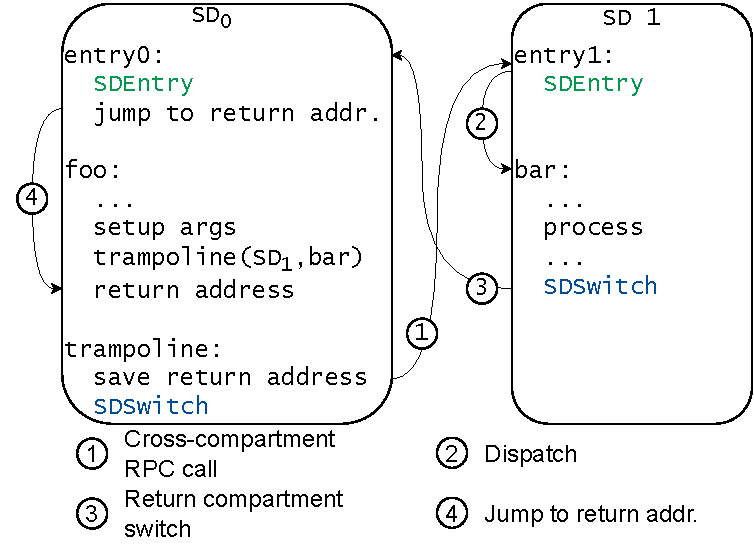
\includegraphics[width=0.7\linewidth]{media/seccells/sc_rpc.pdf}
  \caption{Cross-compartment procedure call in \seccells.}
  \label{fig:seccells:sc_rpc}
  %\Description[<short description>]{<long description>}
\end{figure}

Both forward and return edges on RPC-like cross-compartment 
calls use \sdswitch instructions, as illustrated in \autoref{fig:seccells:sc_rpc} 
where function \Code{foo} makes a cross-compartment call to \Code{bar}.
Arguments are passed in registers.
In this example, the caller uses a trampoline to hide its return address
before switching to \secdivx{1} (Step 1) and uses this address on the 
return path (Step 4).
\secdivx{0} is able to hide its calling address from \secdivx{1}, just
leaking the address of the generic trampoline.
Further, following the return switch to its entry point, \secdivx{0}
can read \rid to verify that the return is indeed from the called 
\secdiv, not any other.
On the other side, the callee (\secdivx{1}) can store its caller and
switch back to the caller's entry point on the backward edge.
If \secdivx{1} contains nested calls to other compartments, it
merely needs to remember its caller somewhere in its memory.
The dispatch (Step 2) secures the forward edge to \Code{bar} with call
gates.
While this example is secure, the flexibility of software allows other
calling patterns.

Context isolation requires the caller to save non-argument/return
registers to a state store before a \sdswitch and restore the same state
on the return edge.
The second step (context restore) is challenging since it
requires the \secdiv to find its state store without trusting any
register state, since the register state prior to the \sdswitch
persists.
We propose an array of per-\secdiv private \cell{}s as 
state stores, indexed by \sid.
The base of this array is easily constructed with
instruction pointer-relative instructions following an entry point.
Simple arithmetic involving the readable \sid register allows
a \secdiv to locate its state store, and consequently restore
the register state.
The latency of in-software context saving to memory is limited by 
the core's bandwidth to the L1 cache, the same as for any potential
hardware implementation.
Therefore, delegating this operation to software has no performance
impact.
Context switching also switches the stack pointer between 
per-compartment private stacks.

%-------------------------------
\subsection{Implementation}
\label{sec:seccells:impl}
%-------------------------------

Our implementation of \seccells augments and modifies the 
RocketChip~\cite{RocketChip} core and firmware.
An overview of the implementation is shown in 
\autoref{fig:seccells:seccell_arch}, with additions to the existing
processor highlighted in grey.
RISC-V provides the ideal, open platform for implementing fully-functional
prototypes of experimental architectures. 
\seccells permits a range of implementations for single and multi-core
processors containing in-order and/or out-of-order cores depending on the 
application's requirements: from firmware implementations on 
low-power embedded processors through hardware or 
microcode implementations on mobile, desktop, and server processors.
We discuss the trade-offs in detail in Appendix~\ref{app:seccells:impl_options}.
To match the RocketChip's simple, in-order pipeline, we implement 
access control and compartment switching in hardware within the pipeline 
and emulate the remaining instructions in firmware.

\seccells provides an alternate virtual memory mode, replacing 
SV-39 and SV-48.
We replace the core's MMU with a range-based TLB and a 
\ptable walker (replacing the traditional page-table walker).
We design the layout of the two-dimensional tables (\ptable and \gtable)
in memory to accelerate cell lookups and maximize 
spatial locality within the cache hierarchy when accessing permissions.
We add \sid and \rid to the core's Control-Status Registers (CSRs), 
and implement \sdswitch in the core pipeline.
The remaining instructions are implemented through hardware-assisted firmware 
by modifying OpenSBI~\cite{OpenSBI}.

The unified \ptable-\gtable in memory starts with a sorted
list of \cell descriptions, followed by the permissions held in the 
\ptable, and then the mappings for the \gtable.
% We don't have this layout any more
Appendix~\ref{app:seccells:ptable} shows the layout in detail.
Each \cell is described by the base and bound virtual addresses, 
the corresponding physical address base, and a single bit denoting
validity.
The sorted list of \cell{} descriptions allows the \ptable walker to
perform a binary search when looking for the cell which contains a particular
address, greatly accelerating lookups.
The row-major layout of the \ptable groups permissions for the same \secdiv
in contiguous cache lines, resulting in intra-cache line spatial locality for
permission lookups, and synergizing well with next-line prefetchers.
As a result, most MMU permission lookups are likely to be served by the L1 cache.
The unified \ptable-\gtable together occupies $\sim160kB$ to track permissions
to 1024 \cell{}s with 64 \secdiv{}s, equal to the memory used by leaf 
page-table entries to map $80$MB of data.

The range-based lookaside buffer holds a few \cell{} descriptions
and the corresponding permissions tagged by \sid.
The implementation of these structures is inspired by recent forays into 
range-based translation caches~\cite{0003BOBFP21midgard, YanLNB19, BasuGCHS13}, 
primarily aimed at tackling the limited reach of modern page-based translation 
lookaside buffers (TLBs).
Midgard~\cite{0003BOBFP21midgard} has shown that such lookaside buffers can 
sufficiently cover the working set of large applications with a 
few ($\sim$ 16) entries.

\seccells' userspace instructions are implemented through 
hardware-software co-design.
The \sdswitch instruction is implemented purely in hardware, and the
remaining permission-modifying instructions are emulated through firmware.
Additional hardware helpers, designed to aid operations trivially achieved
in hardware but costly in software, simplify and accelerate the emulation.
One notable operation is the lookup of the cell's index in the 
\ptable, which is common for all added instructions.
While a binary search in software is expensive, the MMU already holds this
information. 
We add an instruction, only accessible in RISC-V's machine mode and similar 
to the \Code{AT} instruction in ARMv8-A ISA~\cite{ARMAT}, to directly query the MMU.
We envision that higher performance processors with microcode sequencers
can implement these instructions in microcode, and
leave the investigation of the requirements of such an implementation
to future work.

%%%%%%%%%%%%%%%%%%%%%%%%%%%%%%%%
\section{Evaluation}
\label{sec:seccells:evaluation}
%%%%%%%%%%%%%%%%%%%%%%%%%%%%%%%%

In this section, we evaluate key metrics for \seccells' security and 
performance.
First, we show how \seccells provides security for the Browser described
in \autoref{sec:seccells:reqs}.
Second, we measure the latency of the \seccells' userspace instructions 
in microbenchmarks, particularly comparing compartment switching latency 
to related work.
We finally measure \seccells' performance for two representative workloads
highlighting the effect of range-based access control and
using userspace instructions for compartment switching and permissions
transfer.

\begin{table}
  \centering
  \caption{HW configuration of the \seccells prototype. }
  \begin{tabular}{l|c|c}
    \toprule
    Component             & \multicolumn{2}{c}{Configuration}                              \\
                          & Baseline                      & \seccells                      \\
    \midrule
    Core                  & \multicolumn{2}{c}{1 $\times$ Rocket, 6-stage, in-order}       \\
    L1 - D/I TLB          &  32-entry, fully-assoc.       & 16(D)/8(I)-entry, fully-assoc. \\
    L2 TLB                & 1024-entry, 4-way assoc.      & 32-entry, fully-assoc.         \\
    L1 D/I-cache          & \multicolumn{2}{c}{32KB, 8-way associative }                   \\
    L2 cache              & \multicolumn{2}{c}{16MB, 16-way associative}                   \\
    Main memory           & \multicolumn{2}{c}{DDR3, 800MHz, 1GB       }                   \\
    \bottomrule
  \end{tabular}
  \label{tab:seccells:testbench_cfg}
\end{table}



\begin{table}
  \centering
  \caption{FPGA resource utilization for SecureCells' MMU }
  \begin{tabular}{l | r  r  r | r  r  r}
    \toprule
                 & \multicolumn{3}{c|}{Traditional}  & \multicolumn{3}{c}{\seccells}  \\
                 & LUTs   & FFs   & SRAM             & LUTs & FFs   & SRAM            \\
    \midrule
    L1 ITLB      & 1915   & 1886  & 0                & 1529 &  869  & 0               \\
    L1 DTLB      & 2613   & 2048  & 0                & 1272 & 1903  & 0               \\
%   L2 TLB       & ----   & ----  & -                & ---- & ----  & -               \\
    L2 TLB + PTW & 5000   & 3428  & 18KiB            & 3826 & 4596  & 0               \\
%   Total(Core)  & ----   & ----  & -                & ---- & ----  & -               \\
    \midrule
    % \rowstyle{\bfseries}
    MMU Total    & 9528   & 7362  & 18KiB            & 6627 & 6200  & 0               \\
    \bottomrule
  \end{tabular}
  \label{tab:seccells:fpga_resource}
\end{table}

\paragraph{Testbench}
We ran the security evaluation on a QEMU implementation of \seccells,
which faithfully models its functional behavior, and the performance 
experiments on our hardware implementation of \seccells,
which uses cycle-accurate Register-Transfer Level (RTL) simulation to
accurately measure its timing behavior.
The core configuration, described in \autoref{tab:seccells:testbench_cfg}, 
resembles ARM's Cortex-A75. %~\cite{CortexA75}.
Our baseline is an identical core using a traditional page-based MMU
and TLBs instead of \seccells.
\autoref{tab:seccells:fpga_resource} shows the FPGA resource utilization for both the
baseline and \seccells MMUs.
\seccells' \ptable walker contains simpler logic than the baseline, 
as evidenced by the fewer LUTs required in the design.
Additionally, the much smaller range TLB eliminates the 18KiB block SRAM
required to store $1,024$ entries in the baseline L2 TLB.
We run our benchmarks on a seL4 kernel ported to use \seccells' 
memory protections. To evaluate realistic workloads on the seL4 kernel,
we faithfully ported core functionality of benchmarks, carefully limiting
system calls.

%-------------------------------
\subsection{Security Evaluation}
\label{sec:seccells:evaluation:sec}
%-------------------------------

To evaluate \seccells' security claims, we test that a properly 
compartmentalized \seccells program prevents common attack vectors
for monolithic software.
We also include an in-depth analysis of \seccells' instruction semantics
afterwards.

\paragraph{Access Control}
We evaluate \seccells' access control on a mock Browser,
modeling the example described in \autoref{sec:seccells:reqs}.
The Browser contains a simple compiler Engine that generates code for
sandboxed WebApp applications.
The WebApp can allocate arrays, and read/write elements in the array through
get/set instructions.
We emulate a buggy Engine that generates vulnerable WebApp code lacking bounds 
checks on array accesses, allowing the WebApp arbitrary reads and writes.
With the monolithic Browser, an attacker WebApp could leak/modify the
Engine's data as well as that of a second sandboxed WebApp.
When compartmentalized with \seccells with the permissions shown in 
\autoref{fig:seccells:browser_eg}, illegal accesses by the attacker WebApp outside its
data \cell instead raise load/store access faults.
\seccells' access control also prevents arbitrary code injection by the WebApp
by preventing the WebApp from writing to either its or the Engine's code regions.

\paragraph{Context Isolation and Call Gates}
When uncompartmentalized, the WebApp can modify the Engine's stack enabling
control- and data-flow attacks like ROP~\cite{Shacham07}.
Using \seccells for separation, inter-compartment calls between the 
Engine and the WebApp are protected through call gates 
implementing context isolation (\autoref{sec:seccells:design:softmech}) including
stack switching.
\seccells successfully prevents the WebApp from accessing the Engine's stack.

\subsubsection{Formal Description and Analysis of \seccells' 
Userspace Instructions}

We define the semantics of \seccells' unprivileged instructions
in \autoref{fig:seccells:seccell_ops_formal} and discuss their corresponding
security checks below.

\paragraph{\sdswitch}
This instruction checks that the jump target is valid, and holds
an \sdentry instruction executable by the target \secdiv.
With the precondition that the caller \secdiv does not have
writable permission to any \cell executable by the target \secdiv,
\sdswitch guarantees compartment entry at previously defined entry 
points (helping implement call gates). 

\paragraph{\scprot}
This instruction checks that the target \cell is accessible by the
\secdiv, and the new permissions are a subset of the existing permissions.
After this instruction, the \secdiv is assured to have no more permissions
than before.

\paragraph{\scgrant, \screcv and \sctfer}
\scgrant checks that the granting \secdiv has permissions to the
\cell, and that the granted permissions are a subset of its existing
permissions.
\screcv, in turn, checks that the \secdiv is receiving permissions for a
valid cell, that the permissions were previously granted by the
specific \secdiv that the receiving \secdiv expects, and that the received
permissions are a subset of the permissions granted.
\sctfer includes the checks of both \scgrant and \scprot.
The granting and receiving \secdiv{}s must cooperate in order to
transfer permissions, and together finish with the same or fewer
permissions than they began with.

A correct compartment is defined to not grant or receive any permissions 
or invalidate cells that it is not required to grant as per a correct
compartmentalization policy.
Considering a set of compromised attacker \secdiv{}s and their permissions 
to \cell{}s and assuming that uncompromised compartments are correct,
\seccells guarantees that the attackers can neither gain any new permissions 
through any sequence of permission transfer instructions 
nor elevate the permissions of any uncompromised compartment.
Using \scgrant and \screcv instructions, the compromised compartments can
transfer permissions between themselves but those grants cannot include 
permissions which none of the attackers had initially.
The only way for the attackers to gain permissions is from
an uncompromised \secdiv either granting permissions to a \cell or from 
invalidating a private \cell which one of the attackers can validate with \screval.
The only way for the attackers to inject permissions is to have an
uncompromised \secdiv receive them.
By definition, uncompromised compartments will do neither of the above.
Once again, we stress on the importance of a correct compartmentalization
policy.
No mechanism, including \seccells, can protect against an insecure policy
where compartments transfer permissions from/to untrusted compartments
without proper validation.

\paragraph{\scinval} 
This instruction allows a \secdiv to invalidate a \cell to which
it has exclusive access, and to which no outstanding permission grants
exist.
The first condition can be true for a private region, or for one
which other \secdiv{}s have willingly dropped permissions.
Consequently, no other \secdiv will unwittingly lose permissions to
the invalidated \cell as a consequence of \scinval.
The second condition provides the assurance that no compartment can
regain permissions to the cell without executing \screval.

\paragraph{\screval} 
This instruction checks that the address corresponds to an existing 
\cell{} and that it is currently invalid. 
Due to the initial invalidity of the \cell, no \secdiv{}s could have
access to the cell to be revalidated.

\paragraph{\scexcl}
This instruction does not modify any permissions, only allowing a
\secdiv{} to check if it has exclusive access to a \cell{} to which
it already has access to.


%-------------------------------
\subsection{Performance Microbenchmarks}
\label{sec:seccells:evaluation:perf}
%-------------------------------

% Comments on CHERI accounting:
% CHERI provided fine-grained overhead breakdown, which does not strictly
% conform to the
% categories in the aforementioned table. Therefore, we did need to figure
% out how to
% assign costs to categories. Therefore, the method is:
% Fixed costs       = kernel(receive trap) + kernel(exit kernel)
% context switching = caller + libcheri + kernel(clear non-arg registers)
% Switching cost    = Kernel SW operations
%       Switch	Ctx-switch	Other
%   42          42                       caller: Setup call, clear unused argument regs
%   34          34                       libcheri: Save callee-save regs, push call frame  
%   28  28                               kernel: Receive trap                               
%   79  79                               kernel: Validate CCall args.                       
%   41  41                               kernel: Push trusted stack, unseal CCall args.     
%   4   4                                kernel: Clear non-argument registers               
%   12  12                               kernel: Exit kernel                    
%   31  31                               kernel: Receive trap                               
%   7   7                                kernel: Validate return capability                 
%   4   4                                kernel: Clear non-return registers                  
%   41  41                               kernel: Pop trusted stack                          
%   7   7                                kernel: Exit kernel                                        
%   52          52                       libcheri: Pop call frame, restore regs.   
%   1           1                        caller: Back in caller                              
%--------------------------------------------------------------
%       254     129                      Total

\begin{table}
  \centering
  \caption{Compartment switching cost of \\various compartmentalization mechanisms.}
  \begin{threeparttable}
    \begin{tabular}{l | r | r | r | l | l}
      \toprule
                  & \multicolumn{3}{c|}{Round-trip Cycles}               & \multicolumn{2}{c}{CPU}   \\
                  & Switch         & \parbox[t]{1cm}{Context\\                                         
                                                     Saving}    & Total  & OoO\tnote{1} & Model      \\\midrule
      $lwC$       & \multicolumn{2}{c|}{$2 \times 6000$}        & 12000  & \checkmark   & SkyLake    \\
      seL4        & \multicolumn{2}{c|}{$2 \times 514 $}        & 1027   &              & RocketChip \\
      CHERI       & 254\tnote{2}   & 129\tnote{3}               & 425    &              & CHERI      \\
      ERIM        & $2 \times 99$  & Opt\tnote{5}               & 198    & \checkmark   & Xeon       \\
      XPC         & 82\tnote{4}    & Opt\tnote{5}               & 82     &              & RocketChip \\
      \seccells   & $2 \times 8$   & Opt\tnote{5}               & 16     &              & RocketChip \\
      \bottomrule
    \end{tabular}
    \begin{tablenotes}
      \item[1] Out-of-order CPUs incur higher pipeline serialization costs
      \item[2] In-kernel time
      \item[3] Userspace time (caller, libcheri)
      \item[4] XPC call + return + TLB miss
      \item[5] Optional, software-implemented context switch
    \end{tablenotes}
  \end{threeparttable}
  \label{tab:seccells:ipc}
\end{table}

\begin{table}[]
  \centering
  \caption{Cycles for emulating \seccells instructions.}
  \begin{tabular}{l | r | r | r | r}
    \toprule
    Instruction & \parbox[t]{0.7cm}{Trap\\ entry} 
                            & Dispatch  & Emulation & \parbox[t]{0.8cm}{Total \\Cycles} \\
    \midrule
    \scprot     & 79        &   32      &   33      & 144 \\
    \scinval    & 79        &   35      &   68      & 182 \\
    \screval    & 79        &   39      &   44      & 162 \\
    \screcv     & 79        &   54      &   69      & 202 \\
    \scgrant    & 79        &   52      &   63      & 194 \\
    \sctfer     & 79        &   61      &   62      & 202 \\
    \scexcl     & 79        &   57      &   67      & 203 \\
    \bottomrule
  \end{tabular}
  \label{tab:seccells:emulation}
\end{table}

First, we create microbenchmarks to measure the latency of each
userspace instruction introduced by \seccells, of which \sdswitch
is directly implemented in hardware, and the other instructions
are emulated in firmware.

In \autoref{tab:seccells:ipc}, we compare \seccells' compartment switching
cost with that of related mechanisms, particularly for a
round-trip cross-compartment call.
\seccells' userspace \sdswitch enables 8-cycle compartment switches,
with optional software context saving costs, which is more than $5\times$
faster than XPC's switch.
\sdswitch's latency consists of pipeline serialization (5 cycles), 
an instruction permission check (2 cycles) and a single cycle for the
targeted \sdentry instruction.
Of course, both XPC and \seccells would incur higher pipeline serialization
costs on an out-of-order core, putting \seccells on par with, or better than,
the MPK-based ERIM. 
Note that ERIM requires stringent code integrity and control-flow
integrity guarantees while \seccells does not impose any code requirements for
its compartmentalization guarantees.

All instructions other than \sdswitch and \sdentry are emulated by
the firmware, and therefore incur the costs of context saving, 
firmware entry and exit handlers, and dispatch to the correct
emulation function.
\autoref{tab:seccells:emulation} shows the latency of each instruction,
breaking down the cycles spent on each of the above overheads.
A microcode implementation of \seccells would allow the core to use 
internal registers for storage, eliminating the context switch, 
and directly lookup the microcode ROM to find the emulation 
microcode, eliminating dispatch.
Consequently, a microcode-based implementation would reduce 
\seccells' cost to that of the core emulation code only.

%-------------------------------
\subsection{Compartment Switching and Access Control}
%-------------------------------
To evaluate \seccells' practical performance, we create a simplified 
benchmark representative of a popular server workload, 
\Code{memcached}, accurately modelling the workload's memory access 
patterns across varying dataset sizes.
Our benchmark implements the core hashtable-based storage and the 
common query path loaded by an in-process load generator function
and omits system call-dependent features (networking, dynamic resizing),
and the global LRU list.
The benchmark isolates the data store from the vulnerable external interface
--- attackers might send malformed requests to trick the interface into directly
accessing the data store ---
by assigning them to separate \secdiv{}s.
The interface deserializes incoming requests, queries the data store
by switching compartments using \sdswitch, and serializes the
outgoing response.
For simplicity, this benchmark utilizes the migrating thread model.

\begin{figure}
  \centering
  \includegraphics[width=0.85\linewidth]{data/seccells/32ksim/mycached_full.pdf}
  \caption[\seccells performance comparison: \Code{memcached}]
          {Comparison of cycles-per-request,   
          cycles-per-instruction (CPI), and
          TLB miss rate
          while executing compartmentalized \Code{memcached} benchmark on 
          \seccells, compared to the uncompartmentalized version on RocketChip
          (lower is better).
          }
  \label{fig:seccells:mycached_cpi}
  %\Description[<short description>]{<long description>}
\end{figure}

Compartmentalizing the server allows us to measure the overheads
of frequent compartment switches, while varying the program's
dataset size allows us to compare \seccells' scalability.
We scale the dataset size by sweeping the number of fixed-size (64B)
entries stored in the data store, all of which are accessed randomly
by the load generator.
We compare the compartmentalized server running on \seccells'
implementation to an uncompartmentalized server running on
an unmodified RocketChip core by measuring the average count of
instructions retired and cycles used to process each request.
To compare against another emerging compartmentalization architecture,
we also conservatively model CHERI's performance on this benchmark,
adding the costs of supervisor-mediated compartment
switches with hardware support, as reported in the 
CHERI paper~\cite{WatsonWNMACDDGL15}.
We model each compartment switch as 191 instructions requiring 254 cycles,
excluding the costs of context switching and
ignoring other microarchitectural overheads.
In \autoref{fig:seccells:mycached_cpi}, we plot the average per-request 
cycle count and the cycles-per-instruction (CPI) for the server.

\seccells implements fast compartment switching, and 
the cost of switching to and from the data store compartment
for each request (16 cycles) is minuscule ($< 3\%$) compared to the
request processing time (minimum 532 cycles).
Consequently, \seccells' performance closely tracks that of 
the baseline even for small dataset sizes.
In contrast, CHERI's compartment switching overwhelms the
request processing time, only approaching the baseline's
performance for large dataset sizes.
While CHERI's performance for compartmentalization compares
favorably to that of traditional OS-based isolation 
techniques, it offers unacceptable overheads for finer, 
function-granularity compartmentalization (up to 95.5\%).

The CPI graph highlights the baseline system's limited TLB 
reach.
As the dataset exceeds the TLB reach of 4MB, the baseline starts
to encounter TLB misses on accesses to the data store.
Consequently, the baseline CPI starts to degrade compared to
\seccells, and only worsens as the dataset increases past the
CPU's last-level cache capacity.
In contrast, \seccells' range-based lookaside buffer comfortably
scales to large datasets, allowing the \Code{memcached} server to
serve requests 9.3\% faster for a 32MB dataset.
 
%-------------------------------
\subsection{Compartmentalized pipeline}
%-------------------------------

\begin{figure}
  \centering
  \includegraphics[width=0.85\linewidth]{data/seccells/network_1ktlb_sim/nfv_full.pdf}
  \caption[\seccells performance comparison: Network function]
          {Packet processing cycles-per-byte comparison.}
  \label{fig:seccells:nfv_cpb}
  %\Description[<short description>]{<long description>}
\end{figure}

To illustrate \seccells' zero-copy permission transfer performance,
we implement the virtual network function pipeline presented in
\autoref{fig:seccells:dataflow_app}.
The Driver stage generates a ``packet'' by writing a UDP/IP packet
of varying length into a packet buffer, whereas 
the Firewall and NAT read and modify the IP and UDP headers
respectively, but ignore the packet's payload.

Representing the ideal performance target,  we include the
``uncompartmentalized'' configuration that passes the packet by 
reference, incurring no overheads for data transfer.
The second configuration, ``compartmentalized-copy'', 
compartmentalizes pipeline stages and uses shared buffers to transfer
packets by copy.
The third, zero-copy ``\seccells ZC''  configuration isolates
stages, and uses userspace instructions to transfer 
access permissions to packets, each of which occupies a
different \cell{}.
Finally, the ``\seccells ZC-$\mu$code'' configuration models the 
possible performance of a microcode implementation of \seccells' 
dataflow instructions by mitigating trapping overheads
to the firmware and dispatch.
This model is conservative, ignoring possible optimizations from
parallelizing checks in microcode.

In \autoref{fig:seccells:nfv_cpb}, we plot the average number of cycles
required by the benchmark to process a byte of a packet
as the packet size grows.
Fixed costs, such as a function call, compartment switch or 
permission transfer, have diminishing impacts as the packet size grows.
The costs for generating and copying the packet, however, grows
linearly with packet size, and add a constant vertical offset in the
graph.
The ``compartmentalized-copy'' configuration incurs additional costs over the
uncompartmentalized baseline due to 
compartment switches (4.4\% for small packets) and packet copy (51.1\%).
The ``\seccells ZC'' configuration trades-off linearly-growing 
packet copying costs with fixed-cost permission transfers and
(in)validations.
While the $\sim250$-cycle average latency of \seccells' 
permission-modifying instructions causes a massive 199\% overhead
for the smallest packets, this fixed cost quickly gets amortized
for larger packets.
Indeed, this configuration overtakes the ``compartmentalized-copy'' configuration
for 600B packets and above, and approaches the performance
of the uncompartmentalized configuration (2.0\% overhead) for
16kB packets.
Finally, the ``\seccells ZC-$\mu$code'' configuration highlights \seccells'
performance potential, with (average) 69-cycle operations for 
transferring permissions which lowers the break-even threshold to
200B packets.

%%%%%%%%%%%%%%%%%%%%%%%%%%%%%%%%
\section{Related Work}
\label{sec:seccells:related}
%%%%%%%%%%%%%%%%%%%%%%%%%%%%%%%%

A variety of compartmentalization techniques exist, both in software and
leveraging hardware, targeting differing goals and with consequently
different designs.

Attacks often target specific, sensitive data for 
leakage or corruption (e.g., keys or flags).
Consequently, various proposals such as IMIX~\cite{FrassettoJLS18},
ERIM~\cite{ERIMOberwagner19}, and MemSentry~\cite{KoningCBGA17} introduced 
mechanisms to specifically protect 
such data from untrusted or unsafe code.
However, these mechanisms fail to apply to more generic scenarios,
with more than two compartments, per-compartment sensitive or private
data, and non-hierarchical trust models.
COde-centric memory DOMains~\cite{VilanovaBNEV14} proposed an architecture
where the instruction pointer identifies the running compartment, in a bid
to isolate untrusted libraries.
However, this proposal is unable to support the extensive code sharing 
in modern programs, including shared libraries like \Code{libc}.

Compatibility with existing systems brings immediate security benefits.
By mapping the same physical pages across separate per-compartment page 
tables with different permissions, the existing virtual memory implementation
can mimic intra-address space compartmentalization.
Typically, such mechanisms require costly supervisor intervention to
switch compartments limiting the temporal granularity of compartmentalization.
SMV~\cite{HsuHEP16} introduced an API for creating intra-address space
memory views, but relied on the supervisor for compartment transitions.
Light-Weight Contexts~($lwC$)~\cite{LittonVE0BD16} proposed a new OS 
abstraction enabling a fast-path in the supervisor for compartment switching,
essentially eliminating overheads from unnecessary tasks such as scheduling.
$lwC$ successfully reduces the cost of a compartment switch from 4 to 2$\mu$s,
but remains an order of magnitude away from nanosecond-scale switching.
Hodor~\cite{HedayatiGJCSSM19Hodor} uses the VMFUNC instruction, 
introduced for virtual machines, to instead switch page tables in a few 
hundred cycles, eliminating supervisor overheads but consequently
inherits the additional costs of two-dimensional page table walks.
LOTRx86~\cite{LeeSK18} repurposed unused x86 rings to introduce a
privileged userspace for storing sensitive data.
XPC~\cite{DuHXZC19XPC} prioritized software compatibility, choosing to
accelerate the remote-procedure call (RPC) interface used for 
process-based compartmentalization with new userspace instructions.
To achieve this goal, XPC cores track a complicated system of metadata across the
cores and memory, storing a list of compartments, entry points, valid
caller-callee pairs, and a caller stack.
XPC is secure, performant, and can allow exclusive access to a single
data memory range at almost zero cost.
However, XPC requires additional caches for dedicated storage of its
metadata, does not allow permissions to be transferred, and requires
hardware to implement features cheaply implementable in software 
(e.g., call stacks), and cannot support non-RPC like compartment
switches.
With page table-based virtual memory, such proposals all inevitably suffer 
from the scalability limitations of modern TLBs~\cite{PhamVJB12, YanLNB19, 
BasuGCHS13}.

Existing architectures have introduced features for intra-address
space isolation, e.g., Intel's MPK and ARM's MTE extensions,
with fast compartment switching ($<100$ cycles) in the common case.
These extensions enforce additional permissions, but
are insecure under stronger threat models due to designs which
prioritize compatibility with existing processors.
MPK, for example, is defeated by arbitrary code injection.
ERIM~\cite{ERIMOberwagner19} requires complicated code scanning to
prevent code injection, and Donky~\cite{SchrammelWSS0MG20Donky} requires 
hardware modifications to introduce an additional trusted privilege level 
within userspace.
Since neither ERIM nor Donky validates code accesses, an attacker
targeting cross-compartment code injection need not make the
malicious code executable for the target before tricking the target 
into executing this code.
Memory keys also architecturally limit the number of memory regions for 
which permissions can be efficiently tracked, leaving no room for future 
microarchitectural advances to improve code performance.
These systems also inherit the TLB-reach issues of modern TLBs.

Range-based permission tracking tackling the TLB-reach issue 
appeared in Mondrian Memory Protection (MMP)~\cite{WitchelCA02MMP}.
MMP proposed a virtual memory architecture tracking segment-based 
permissions for compartments within an address space, 
simulating zero-copy for networking through redundant mappings for
packet buffers with different, static permissions.
MMP only implements access permission checks in hardware, 
delegating other operations, including compartment switches, 
to the supervisor, precluding high-performance applications.
MMP also uses different permissions tables for each compartment,
reading duplicated range boundaries on each switch.

CHERI refers to hardware-enforced memory capabilities~\cite{WoodruffWCMADLNNR14}, 
and an eponymous compartmentalization mechanism reusing the same 
capabilities~\cite{WatsonWNMACDDGL15}.
The original proposal for memory capabilities offers a practical
mechanism to mitigate spatial safety bugs,
restricting the ability of pointers to access memory beyond bounds.
We recognize that CHERI's capabilities can prevent memory corruption within
a compartment, motivating integration  with \seccells
to together improve security.
CHERI compartmentalization encapsulates capabilities to a compartment's
code and data, relying on costly supervisor-mediated compartment switches.
CHERI lacks auditability since capabilities are spread throughout
memory, and a bug resulting in a capability being leaked cannot be cheaply
detected and fixed.
CHERI's switching costs are not security-proportional, lacking the
ability to skip context switching costs when acceptable.
Finally, CHERI's permissions are built on traditional page-based translations,
and inherit TLB limitations.
Nonetheless, CHERI allows more granular per-object capabilities as compared
to \seccells' per-VMA permissions.
% The distributed nature of permissions also means that a compartment
% can never be assured of exclusive access to a memory region and also
% implies a memory overhead
% proportional to the number of capabilities stored in program memory.

Along with mechanisms, policy research is equally important.
Researchers have attempted to formalize a compartment program's 
guarantees~\cite{JuglaretHAEP16}, determine the scope of access following
permission transfers under the take-grant model~\cite{LiptonS77},
automatically infer isolation policies from 
programs~\cite{RoesslerAPMPKPB21,KirthDCLDGNVF22,VasilakisKRDDS17},
provide hints to programmers on isolation boundaries based on
automated analysis~\cite{GudkaWACDLMNR15}, and
reason about what guarantees remain when one or more compartments are
compromised~\cite{AbateABEFHLPST18}. 

%%%%%%%%%%%%%%%%%%%%
\section{Discussion}
\label{sec:seccells:discussion}
%%%%%%%%%%%%%%%%%%%%

\paragraph{Legacy program/OS support}
\seccells is compatible with existing pre-emptive operating systems which 
already separate architecture-specific memory management code.
\seccells also supports page-based memory management (demand paging, swapping)
when integrated with upcoming intermediate-address space memory 
architectures~\cite{ZhangSRL10,0003BOBFP21midgard}.
Since \seccells preserves the VMA-based view of virtual memory, 
an OS can present a legacy userspace environment for existing monolithic
applications by allocating a single compartment in the \ptable.
Legacy applications will also benefit from \seccells' improved 
TLB-reach with range-based address translations.

\paragraph{Adopting \seccells}
\seccells faces the daunting task of changes across the software and 
hardware stack.
Nonetheless, library and compiler support for software development
can greatly aid developer adoption.
%To evaluate our benchmarks, 
We developed a prototype library
(\Code{scthreads})
to support compartments with isolated contexts, and envision that
most software can be ported through compilation with a
\seccells-compatible C/C++ library.
We compartmentalized the example Browser ($\sim$1kLoC), 
initially developed and tested on an \Code{x86} machine, 
in approximately two additional days.
Software such as browsers desiring the full benefits of compartmentalization
will still require rewriting (to refactor monolithic code into compartments).
\seccells' userspace instructions map to common compartmentalized
applications' operations, evidenced by strong parallels between
\seccells' instructions and APIs in related mechanisms or 
language-level operations in compartmentalization
frameworks (\autoref{tab:seccells:api_mapping}).
This mapping will simplify porting existing compartmentalized
applications, such as Nginx-lwC~\cite{LittonVE0BD16}, to run on \seccells
by replacing existing operations with the \seccells equivalent 
(e.g., substitute \sdswitch in place of \Code{lwSwitch}).
Existing software compartmentalization libraries and compilers~\cite{HsuHEP16}
can also use \seccells as a backing mechanism.
%
For example, consider a \seccells backend for the LitterBox sandbox,
used by the compartmentalizing compiler Enclosures~\cite{GhosnKPLB21}
to isolate untrusted Go libraries, improving performance and security over
the existing Intel VT-x and MPK backends respectively.
Enclosure switching (\Code{Prolog} and \Code{Epilog}) map to \sdswitch
instructions whereas data movement (\Code{transfer}) maps to a 
\sctfer-\screcv pair.

\begin{table}[h]
  \caption{Mapping \seccells instructions to related mechanisms, libraries and language features.}
  \begin{threeparttable}
    \begin{tabularx}{\columnwidth}{p{1.4cm} | >{\raggedright\arraybackslash}X}
    \toprule
      Instruction & Analogous API \\
    \midrule
      \sdswitch  &                                                                                    \Code{dcall}~\tnote{3},                \Code{CCall/CReturn}~\tnote{4}, \Code{Prolog/Epilog}~\tnote{5}, \Code{lwSwitch}~\tnote{6}  \\ %\midrule
      \scprot    &                  \Code{mprotect}\tnote{1},          \Code{mpk_mprotect}~\tnote{2}, \Code{dk_mprotect}~\tnote{3},          \Code{CAndPerm}~\tnote{4}                                                                  \\ %\midrule
      \scinval   &                  \Code{munmap}\tnote{1},            \Code{mpk_free}~\tnote{2},     \Code{dk_munmap}~\tnote{3}                                                                                                        \\ %\midrule
      \screval   &                  \Code{mmap}\tnote{1},              \Code{mpk_mmap}~\tnote{2},     \Code{dk_mmap}~\tnote{3}                                                                                                          \\ %\midrule
      \scgrant \screcv \sctfer &    \Code{mmap(MAP_PRIVATE)}\tnote{1},                                \Code{dk_domain_assign_key}~\tnote{3},                                  \Code{Transfer}~\tnote{5},     \Code{lwOverlay}~\tnote{6} \\ %\midrule
      % \scexcl    & N/A                                                                                                                                                                                                                  \\
    \bottomrule
    \end{tabularx}
    \begin{multicols}{2}
    \begin{tablenotes}
      \item[1] Linux processes
      \item[2] \Code{libmpk}~\cite{ParkLXMK19}
      \item[3] Donky~\cite{SchrammelWSS0MG20Donky}
      \item[4] CHERI~\cite{WatsonWNMACDDGL15,WoodruffWCMADLNNR14}
      \item[5] Enclosures~\cite{GhosnKPLB21}
      \item[6] lwC~\cite{LittonVE0BD16}
    \end{tablenotes}
  \end{multicols}
  \end{threeparttable}
  \label{tab:seccells:api_mapping}
\end{table}

% Possibly remove for resubmission
% Bring back for camera ready
\paragraph{System call semantics with \seccells}
Recent work~\cite{ConnorMSS20} has demonstrated that the Linux system call
interface can be used to compromise userspace compartmentalization.
Modifications of the syscall interface, such as those proposed in 
Jenny~\cite{schrammel2022jenny}, are orthogonal to the compartmentalization
mechanism and can be applied to \seccells.
We leave a systematic evaluation of kernel performance and 
system call semantics with \seccells to future work.

\paragraph{Advantages for microkernels and system calls}
Fast compartmentalization is the key objective for practical microkernel
operating systems.
By running the OS kernel and drivers in \secdiv{}s, \seccells improves over
a modern microkernel's switching time by two orders of magnitude.
Similarly, userspace programs can benefit from significantly faster system
calls if the kernel is assigned a compartment within each program's address
space.
Essentially, the costly system call entrances can be replaced by cheaper
\sdswitch instructions into the kernel.  

\paragraph{Speculative-execution attacks (SEA)}
We consider the threat of speculative side-channel attacks like 
Spectre~\cite{KocherHFGGHHLM019} in \seccells' design, despite 
omitting such attacks from our attacker model.
\seccells{} introduces additional mechanisms for changing an executing
thread's permissions, through userspace compartment switching and
permission transfers.
Fault-based attacks like Meltdown~\cite{lipp18sec} must be prevented in
implementations by preventing faulting loads from accessing memory or
forwarding their data to subsequent instructions~\cite{WeisseNLWK19}.

\seccells does not mitigate existing SEA, but takes care
not to introduce vulnerabilities.
\seccells specifies that userspace instructions are serializing, 
precluding speculative permission changes.
An attacker cannot, for example, speculatively switch to a victim
\secdiv using an \sdswitch following a long-latency branch and read 
the victim's private data using the victim's permissions.
\seccells' permission transfer instructions are atomic, preventing visibility 
or exploitation of any intermediate permission state.
An attacker \secdiv cannot, for example, drop permissions for a \cell
using \scprot while transferring the same permissions using \sctfer in parallel.
Our firmware (and future microcode) implementation use load-linked 
store-conditional atomic operations commonly available across architectures
to ensure atomicity.


\seccells' access control limits the leakage scope of 
Spectre attacks to a compartment's accessible \cell{}s, 
weakening SEA.
\seccells allows the pipeline to speculate as usual within a compartment's 
execution, and speculative accesses are also subject to access control 
by the MMU and cannot illegally access any \cell.
Access control, therefore, also limits the leakage potential of existing
Spectre gadgets.
Whereas a Spectre gadget on a traditional processor can address and
access any user memory in the process' address space, the same Spectre
gadget can only access memory within the compartment's \cell{}s.
\seccells also limits the code (speculatively) executable within a compartment,
further restricting the availability of Spectre gadgets.


%%%%%%%%%%%%%%%%%%%%%%%%%%%%%%%%
\section{Conclusion}
\label{sec:seccells:conclusion}
%%%%%%%%%%%%%%%%%%%%%%%%%%%%%%%%

Compartmentalization requires labor-intensive code restructuring, 
deterring developers from adopting piecemeal solutions which provide
partial protection or which cripple performance.
This chapter introduces \seccells, a secure, flexible and 
performance-focused compartmentalization architecture to
underpin future software compartmentalization efforts.
Further work is required, for 
scaling our FPGA prototype to an out-of-order, multicore processor, 
investigating implementations of higher-level abstractions 
on \seccells' mechanisms,
developing software conventions to develop correctly
compartmentalized programs for \seccells, 
and to improve OS support for the architecture.

Nevertheless, \seccells enables practical, effective, and efficient
compartmentalization by tackling 
the core architectural requirements for a mechanism.
\seccells strictly enforces access controls and protects permissions
from corruption, while supporting secure 8-cycle compartment switching.
\seccells constrains inter-compartment control flow to respect
call gates, protecting these interfaces from fault propagation.
\seccells is also an enabler for data processing pipelines
with userspace zero-copy data transfers.
\seccells remains flexible, eschewing policy-specific specializations.
We have published the \seccells prototype, benchmarks
and supporting infrastructure
at \url{https://www.hexhive.epfl.ch/securecells}.


%%%%%%%%%%%%%%%%%%%%%%%%%%%%%%%%%%%%%%%%%%%%%%%%%%%%%%%%%%%%%%%%%%%%%
% Compartmentalization Mechanism Review
%%%%%%%%%%%%%%%%%%%%%%%%%%%%%%%%%%%%%%%%%%%%%%%%%%%%%%%%%%%%%%%%%%%%%
\chapter{A Review of Compartmentalization Mechanisms }
\label{ch:compreview}
% \epigraph{Why does the janitor have the nuclear launch codes?}%
%         {\textit{President-sir, probably}}
A compartmentalized program consists of isolated compartments with controlled
communication paths between them, as defined by a 
compartmentalization \emph{policy}.
A compartmentalization \emph{mechanism} is responsible for upholding the
isolation and communication rules as described by the \emph{policy}.
A developer has a choice between a plethora of academic and industrial 
mechanisms\footnotemark
proposed to support compartmentalization.
However, mechanisms differ in the threat models they are designed to protect
against, their performance characteristics, the use cases they support, and
their compatibility with existing or upcoming system architectures.
A survey of compartmentalization mechanisms is required to understand the
properties and guarantees of different proposals, and compare their
suitability for compartmentalization use cases.
In this chapter, we will take a deeper dive into a wide range of 
compartmentalization mechanisms and compare them on security and performance
properties.
\footnotetext{In this chapter, the term ``mechanism'' refers to a 
compartmentalization mechanism.}

%%%%% Parts of this background are already discussed in the SecureCells paper.
%%%%% However, we need not repeat this stuff in this section.
% \section{Background on Compartmentalization}

% \begin{itemize}
%       \item Modern software is monolithic, or compartmentalized at a coarse granularity.
%       \item Monolithic software runs all parts of an application in a single address space
%       \item Issues with monolithic software includes:
%             Memory safety bugs can compromise data throughout the address space
%             Control flow hijack/bending allows any code to call any other code
%             Can lead to system calls being called from unexpected code
% \end{itemize}

% In contrast, a compartmentalized program separates logical components of the application
% and isolates them in individual compartments, which implies some degree of separation.
% Isolation restricts which resources each compartment has access to, in order to prevent
% one or more of the above attack vectors.

% Compartments are logical, and not necessarily linked to code. 
% For example, compartments for a browser can include the JIT compiler, the runtime and the
% untrusted sandbox code. 
% While these are isolated, they may have access to the same code, including libraries like
% libc.
% Additionally, there might be one or more sandboxes which are instances of the same module,
% for example, and thereby share exactly the same code regions. 
% However, they would need to have separate data regions or some isolated contexts.
% All of this is to say that we should not make a 1:1 link between code and compartment.

% The aim of this section is to provide background of compartmentalization as a software design principle to provide enhanced security. 
% This section will explain the terminology of "monolithic" and "compartmentalized" programs. 
% This section will also describe the attacker model for compartmentalization and what attacks can be prevented.


%%%%%%%%%%%%%%%%%%%%%%%%%%%%%%%%
\section{Description of use cases and threats}
\label{sec:compreview:usecases}
%%%%%%%%%%%%%%%%%%%%%%%%%%%%%%%%
In this section, we introduce some characteristic use cases for 
compartmentalization, and 
describe some typical attacker models.
These examples will allow us to compare the mechanisms described later.

%-------------------------------
\subsection{Hierarchical trust} 
\label{sec:compreview:usecases:hierarchical}
%-------------------------------
Let us consider a system with hierarchical notions of trust.
In \autoref{sec:seccells:reqs}, we have already encountered the example of
a browser running untrusted code from a web application.
In this application, the JIT engine creates and orchestrates execution of
the sandboxed code.
The JIT engine has access to the WebApp's code and data region, implying
a hierarchical trust relation ---
the WebApp must trust the Engine to correctly generate code and modify
its data.
Despite this hierarchical trust relationship, 
the Engine's permissions (\Code{rw}) to the WebApp's code is not a
superset of the WebApp's (\Code{rx}).
While the Engine's code is separate from the WebApps, the Engine might allow
the WebApp to directly execute specific shared code from 
libraries (say \Code{memcpy}).
The Engine's OS resources must also be isolated and inaccessible by the
WebApp.
The Engine can ensure that the WebApp code contains no syscalls and interpose
every request to OS resources by the WebApp, or install system call filters
which properly restrict syscalls by the WebApp.
Since the system call interface of modern OS kernels like Linux can be used to 
bypass intra address-space compartmentalization~\cite{ConnorMSS20}, we must
assume that every mechanism below is adapted to run with a kernel which
properly isolates OS resources for each compartment (for example, as proposed 
by Schrammel~et.~al.~\cite{schrammel2022jenny}).
\atri{systems restricted to a single trusted/untrusted compartment won't work}
\atri{systems without system call filtering will fail (does ERIM have filtering?)}
\atri{systems where the kernel cannot identify the caller will fail 
      (does donky prevent OS confused deputy, or allow OS to identify caller?)}
\atri{Systems with hierarchical trust, where superset relation is needed will fail}
\atri{CODOMs' where APL grants full permission for a domain's regions will fail}
\atri{Code = Domain, like CODOMs, will bar cross-compartment code sharing}

Adding to the example from \autoref{sec:seccells:reqs}, consider that the
Engine is sandboxing more than one WebApp from different sources.
The WebApps do not trust each other, and must be isolated from each other.
Each WebApp's memory regions and OS resources.
Further, the WebApps should not be able to directly call each other.
Any interaction between WebApps should pass through the Engine.
\atri{Cross-compartment calling restrictions (if callee can ident itself and caller)}

Common threat models for this browser setup would be to assume a buggy Engine
which either
\begin{inparaenum}[\itshape i\upshape)]
      \item generate an arbitrary read or write primitive in the code generated
            for a WebApp, or 
      \item generate arbitrary attacker controlled code for a WebApp.
\end{inparaenum}
Compartmentalization must, nonetheless, protect the Engine and other WebApp 
from a malicious WebApp which exploits the buggy Engine's code generation.
\atri{How many systems break with arbitrary code exec}

%-------------------------------
\subsection{Mutual distrust} 
\label{sec:compreview:usecases:distrust}
%-------------------------------
A workload similar to \Code{memcached} described in 
\autoref{sec:seccells:evaluation:memcached} can have mutual distrust
between directly communicating compartments.
For this section, we assume that the server's data store (Store) compartment
compartment distrusts the server's networking (Network) compartment and
vice versa.
We assume that a malicious attacker who compromises the Network compartment
can try to attack the Store by calling the Store with a malicious register
context.
For example, the attacker Network can use a malicious stack pointer register 
in order to trick the Store to use a wrong region of memory as its stack.
The Network attacker might try to write one of its data regions with a malicious
stack state and point the Store's stack pointer to this region.
In this attack, the Network wants to use the fake stack state to influence the
Store to compromise its own state or the in-memory database.
Further, the Network attacker would need to share the region hosting the fake
stack with the Store, either beforehand or by dynamically passing its 
permissions before calling into the Store.
In a generalized attack, the malicious register may be any register, not
only the stack pointer.
\atri{CHERI can fail the malicious rsp attack/malicious pointer register attack}.
\atri{Systems requiring hierarchical trust will fail.}
\atri{CODOMs' where APL grants full permission for a domain's regions will fail}

In the case of mutual distrust, compartments must use static threading 
and maintain their own context state.
Particularly, the callee on a cross-compartment call must be able to 
restore a clean, trusted register state before processing the incoming request.
Likewise, the caller must be able to restore its own state when the callee
returns control.
\atri{Systems mandating migrating threading will fail}

%-------------------------------
\subsection{Trusting but wary}
\label{sec:compreview:usecases:wary}
%-------------------------------
A workload such as the network function (NFV) pipeline described in 
\autoref{sec:seccells:reqs} might be developed within a more trusted
ecosystem, and have stronger trust relations between compartments.
Let us again consider a pipeline with multiple stages, each of which
is isolated within a separate compartment.
Data packets get moved between pipeline stages as each stage of the
pipeline executes.
The main goals for the pipeline would be to 
\begin{inparaenum}[\itshape i\upshape)]
      \item prevent bugs in one stage from corrupting a separate stage, 
      \item maintain high packet processing rates in order to satisfy
            the network's line rate, and
      \item maintain high availability, where crashes in parts of the
            pipeline are handled gracefully and with minimal downtime.  
\end{inparaenum}
\atri{Fast compartment switching}
\atri{Fast zero copy data movement}
\atri{kernel needs to be able to identify faulting compartment}

Another popular use case is library compartmentalization, where shared
libraries within an application can be isolated within compartments.
Shared libraries, which are often community developed, feature prominently
in applications but can have bugs which compromise the rest of the
application.
Shared libraries can generally be trusted to not be malicious, but can
have bugs. 
Therefore, the compartmentalization policy can require lighter isolation
rules for shared libraries.
Function calls between libraries can also happen at a high frequency in
applications, so low overhead for switching is required.


%%%%%%%%%%%%%%%%%%%%%%%%%%%%%%%%
\section{Properties}
\label{sec:compreview:properties}
%%%%%%%%%%%%%%%%%%%%%%%%%%%%%%%%

In this section, we describe some of the possible guarantees or protections
that compartmentalization mechanisms can provide.
We will also describe the common operations for compartmentalized programs,
which will allow us to explore the performance potential of different
mechanisms.

%-------------------------------
\subsection{Security Properties}
%-------------------------------
Compartmentalization mechanisms aim to provide mitigations for applications
where one or more compartments have been compromised, specifically opposing
further corruption of remaining compartments or the rest of the system.
As described in \autoref{sec:compreview:usecases:hierarchical}, common threat
models assume that a compromised compartment either gives an attacker arbitrary
memory pointer dereference or arbitrary code execution as that compartment.
In this section, we describe possible security properties and how mechanisms
might provide these properties.
These security properties roughly fall into two categories, those that
perform access control to restrict access to resources and reduce
compartment privileges, and those that secure compartment interfaces
which remain the primary attack vector for inter-compartment fault propagation.
We must assume compartments which harden their interface against attacks
which can be triggered through maliciously crafted arguments, as no
mechanism can fully protect an improperly compartmentalized program.

\atri{We can expand greatly on the consequences of lacking security properties
in this section}
\atri{Me might want to make these shortcomings concrete through examples of
actual attacks}

Compartmentalization prevents direct cross-compartment memory access, by 
defining separate memory address spaces for compartments or by 
enforcing per-compartment access rights for intra-address space compartments.
Mechanisms implement access control through variations of page table entries,
segments, permission tables, protection keys or memory capabilities.
Therefore, a compromised compartment cannot directly leak or corrupt a 
different compartment's memory.
Memory access control can also be used for access control to memory-mapped
I/O.

Memory access control must extend to code fetch besides data read/write
accesses.
Modern programming languages rely on code pointers stored in memory or
registers, and indirect calls and returns which use code pointers.
Without access control on code fetch, a victim compartment might be fooled 
into executing code for a different compartment by merely corrupting a
code pointer used during the victim's execution. 
Malicious code injection can be mitigated with permission checks on the
code fetch paths.

Compartmentalization also controls access to system resources.
Mechanisms can separate namespaces for system resource handlers between
compartments, introduce an interposing layer on system calls or 
implement compartment-aware system call filtering.
Separate namespaces prevent compartments from naming other compartments'
resources (e.g., each process has independent file descriptor tables).
System call interposition or filtering can both prevent compartments from
using some system calls or use syscalls with malicious arguments.
For using system call filtering, the mechanism must enable the kernel to
definitively identify the calling compartment.

When compartments communicate, the inter-compartment calling interface 
represents the primary attack vector for a compartment. 
A minimal requirement is that control flow for cross-compartment calls
must enter a compartment at legal entry points.
Failing this, attackers might be able to mount 
return-oriented programming (ROP)-like attacks which leverage unintended
code sequences to bypass compartmentalization guarantees.
Fixed entry points are also vital to implement call gates, which enable
compartments to implement vital checks at inter-compartment interfaces.
We describe a couple of these checks next.

Compartmentalization should limit which compartments are allowed which other
compartments, as an application of least privilege. 
A sandboxing engine could require, for example, that calls between sandboxes
are interposed by the engine.
To implement this check, mechanisms might track allowed caller-callee 
compartment pairs, and validate each cross-compartment call.
Alternatively, mechanisms can allow compartments to validate their own
callers as part of the call gate.
For the latter, a callee must be able to irrevocably identify itself and its 
caller.

When compartments do not trust each other, a compartmentalization mechanism
must enable compartments to maintain their own contexts (static threading).
Without static threading (migrating threading), the register context following
an inter-compartment call may be malicious.
For example, the stack pointer register could point to a attacker-crafted
malicious stack.
Mechanisms might themselves implement secure context switching at compartment
boundaries, or enable compartments to perform the context switch as part of
call gates.
In the latter case, compartments should be able to fetch their register context
securely without trust on any registers passed after the compartment switch.
Compartments must be able to locate a private state store and
restore context from it.
To locate its private state store, a compartment might need a way to uniquely
and securely identify itself. 

Compartments pass arguments for inter-compartment calls by value, through 
registers, or by reference, through memory.
Data passed through memory might use shared memory buffers, be copied between
private buffers by a privileged entity like the OS kernel, or be passed without
copying if the caller can grant permission to the existing location of the data
in memory to the callee.
The third option, called zero-copy, is particularly necessary for high-performance
applications.
Passing permissions raises security challenges, which mechanisms can try to 
mitigate with the following properties. 
First, no compartment should be able to unilaterally grant or seize permission to 
data to or from another compartment respectively.
If a compartment can unilaterally seize permissions for another compartment's data,
this would trivially break isolation.
A compartment could gain access to, and corrupt, another compartment's private
data.
If a compartment could unilaterally grant permission to another compartment, 
compartments could mount confused deputy attacks where the target compartment may
be tricked into using attacker-crafted data whose permissions were injected into
the target by the attacker.
Particularly, this vector could make inter-compartment code injection trivial.
A secure permission transfer should employ a handshake between the source and
target compartments, who agree to mutually transfer permissions.

\begin{figure}
      \centering
      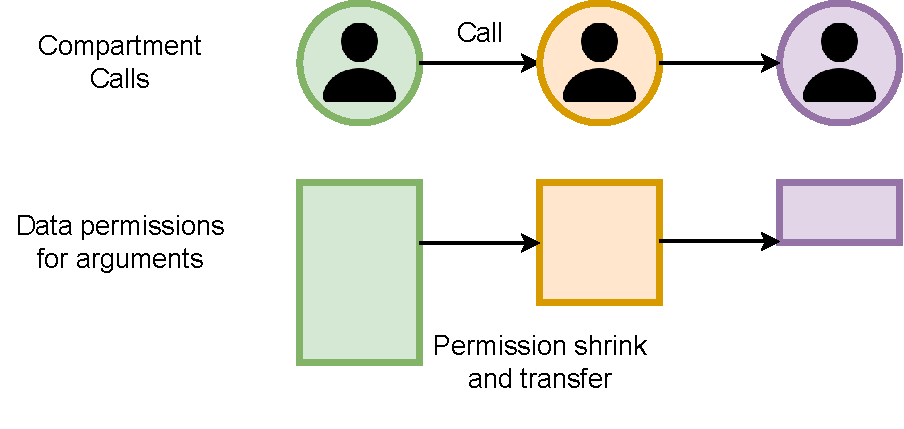
\includegraphics[width=0.75\linewidth]{media/compreview/permission_shrink_grant.pdf}
      \caption{TODO Stuff}
      \label{fig:compreview:permshrink}
\end{figure}
Additional properties are desirable when passing
permissions between compartments - revocation and shrinking permissions.
A compartment should be able to selectively transfer permissions for a 
some, not all, of its memory regions.
A common usage pattern is synchronous permission passing, where a caller
compartment intends to transfer permission to arguments to the callee for the
duration of the callee's execution as a form of temporal least privilege.
A corollary is that the callee should no longer have access to the granted
permissions once the callee returns.
Since the caller may not trust the callee to surrender permissions correctly, 
mechanisms can support revocation to allow the caller to revoke the previously
granted permissions when the callee returns.
During nested compartment calls, the callee for the first call might want to pass
permission to a subset of its arguments to the callee for the second call.
We illustrate this situation in \autoref{fig:compreview:permshrink}.
A mechanism which supports this paradigm securely should allow a compartment to
shrink permissions for a region to create permissions for a smaller region
which can be transferred during the second call. 

When an application has concurrent access to writable data regions shared 
between concurrently executing compartments, data races can emerge due to
improperly synchronized access to shared data.
Attackers can exploit such bugs to compromise interfaces, as described for
example in \autoref{ch:midas}.
To mitigate bugs from shared access to data, a mechanism may temporarily provide
compartments exclusive access to otherwise shared data.

%-------------------------------
\subsection{Performance Properties}
%-------------------------------
The performance of a compartmentalized program depends on the cost of
a mechanism's checks and protections, and on the frequency at which these
overheads are encountered.
In this section, we will generally describe the operations required to
support compartmentalization, explain why they are required and their
frequency of occurence. 
This information will allow us to compare the performance characteristics
of compartmentalized applications across different mechanisms.

First, compartmentalization requires access control to resources, particularly
to memory and to OS resources.
Memory is accessed during instruction fetch and for load and store instructions
at nanosecond scale.
Access control to memory is required for all instruction fetches, and for
loads and stores which account for roughly $35\%$ of retired instructions
for SPEC-int benchmarks on average~\cite{LimayeA18}.
A modern desktop or server processor core runs at 2-4GHz clock speed, and
retires more than 1 instruction per cycle on average, which requires
multiple access control operations per cycle.
A mechanism must also be able to scale with application dataset sizes, as
modern applications use gigabytes to terabytes of memory.
Large datasets stress near-core translation or protection caches, such as
the translation lookaside buffer (TLB) on commercial cores.
Mechanisms which rely on TLBs or similar structures might inherit the
scaling limitations of these structures.
Programs access OS resources, generally requiring a system call, at
relatively relaxed time frames.
While more traditional desktop workloads require system calls at 
millisecond-scale, more high-performance server workloads including the
virtualized network function described in 
\autoref{sec:compreview:usecases:wary} may require system calls to access
the network at microsecond scale.

Second, compartments need to communicate with cross-compartment calls.
Typically, mechanisms implement cross-compartment calls as one hardware
core switching from executing the caller compartment to the callee.
Compartment switching is less frequent compared to access control, happening
at sub-microsecond to millisecond timescales.
For example, unmodified Firefox compartmentalizes at a 
coarse granularity, putting individual tabs in separate processes.
Unmodified Firefox is limited to coarse grained compartments due to the high
micro-second scale cost incurred for inter-compartment calls between
processes.
However, we measured that a finely-compartmentalized Firefox switches between
compartments every 750 instructions on average, 
when compartmentalized with every library occupying a separate compartment.
On a modern processor, 750 instructions executes in less than a microsecond.
Cross-compartment calls must also move data as arguments for the call.
Mechanisms might enable data movement through copying, use of shared memory
between the caller and callee, or by transferring permission for the
data regions holding arguments.
Practically, the cost of compartment switching and data movement informs the 
security-performance tradeoff, 
with lower overhead mechanisms allowing applications to implement
finer-grained compartmentalization while maintaining the same performance.
High-performance software requiring 
compartmentalization~\cite{HwangRW14,MartinsAROHBH14,RamCCR13,HondaHLR15}
relies on unoptimal designs like pinning compartments to cores to skip the
cost of switching compartments on a core and reliance on memory shared between
all compartments to prevent data movement between compartments.
Core pinning wastes core time, as each core typically does not need the same
amount of execution. 
When virtualized network functions are pinned to cores, cores executing stages
with lesser computation must wait for cores executing longer stages.
Memory shared between all stages removes some of the benefit of 
compartmentalization, as a corrupted stage can also corrupt data being 
processed by other stages.

%-------------------------------
\subsection{Usability Properties}
%-------------------------------
Compartmentalization mechanisms optimize for different objectives, and vary
widely in design.
Consequently, mechanisms offer different degrees of usability to application
developers.
Ideally, mechanisms aim to be generic and widely applicable, able to support
a wide array of different use cases allowing varied developers to 
benefit from compartmentalization for their applications.
Mechanisms would also ideally allow compartmentalization with minimal developer
effort, through compiler-based automation.

Mechanisms need to be flexible, supporting different policies.
We have discussed use cases with different trust relationships in 
\autoref{sec:compreview:usecases}.
Mechanisms which optimize for sandboxing, for example, might assume
a hierarchy of trust with the sandboxing runtime being most trusted
and sandboxes being untrusted.
A mechanism which only allows hierarchical compartments, however,
will not be able to support relations with mutual distrust between
compartments.
Flexibility also applies to inter-compartment calls, and to the requisite
control or data flows.
Applications might require standard call-and-return control flow,
nested compartment calls, or asymmetric control flow without returns.
When transferring data between compartments, mechanisms should allow
fine-grained spatial definition of data transferred.
Mechanisms which transfer data at fixed granularities, for example a
4 kilobyte page, would be unoptimal.

A mechanism should also integrate with existing and future software and
hardware systems, i.e., maximize compatibility.
Backward compatibility, for example, allows the plethora of existing systems
to use the mechanism with less effort compared to a 
mechanism with a clean-slate design.
As a trade-off, a backward compatible mechanism might inherit shortcomings
of existing mechanisms and may not be usable on newer systems.
In contrast, a forward compatible mechanism would be designed for working
with upcoming or future systems rather than existing ones.

Mechanisms which can automatically compartmentalize existing applications
benefit developers immensely.
Compartmentalization requires principled design of the isolation policy,
and generally requires invasive changes to port over existing monolithic
applications.
As complex applications scale to millions of lines of code,
principled compartmentalization often becomes too expensive.
Automated compartmentalization techniques generally implement weaker
security guarantees compared to manual, principled compartmentalization,
but greatly reduces the cost of adding compartmentalization.
In many cases, automated compartmentalization may be the only 
cost-feasible solution, and the weaker isolation provided is still
safer than monolithic applications.

%%%%%%%%%%%%%%%%%%%%%%%%%%%%%%%%
% Introducing the surveyed mechanisms
\section{Compartmentalization Mechanisms}
\label{sec:compreview:mechanisms}
%%%%%%%%%%%%%%%%%%%%%%%%%%%%%%%%

To understand and compare mechanisms, we first need to understand each 
mechanism, and understand their model for compartmentalization.
In this section, we will describe relevant compartmentalization mechanisms
and summarize their key features.
We will also try to explore their abstractions and isolation model,
and illustrate what compartmentalized programs look like under that model.
Finally, we will try to illustrate how a browser 
(described in \autoref{sec:compreview:usecases:hierarchical}) is 
compartmentalized with each mechanism to protect the JIT engine from
untrusted web application code.

%-------------------------------
\subsection{Process-based compartmentalization}
%-------------------------------

The traditional abstraction of isolation is based on processes.
We will describe process-based compartmentalization in UNIX-like OSs
(particularly Linux), 
though the concepts generalize to other OS kernels.

% Context about how processes emerged
The process abstraction was introduced to isolate programs running on 
multi-user machines.
Each process has an isolated memory space (architecturally-defined virtual memory)
and individual OS resources, such as file descriptors, I/O handles or capabilities.
The OS kernel time-multiplexes processes onto one or more processing cores.
A process can have one or more kernel threads, corresponding to independent threads
of execution, but sharing the same address space and OS resources.
Everything within a process shares the same permissions to access its memory and
its OS resources, including the program's executable, libraries, and loaded modules.

% Explain how processes allow compartmentalization
To compartmentalize a program, that program needs to isolate each compartment in
a separate process.
% Isolation part.
Each process will have its own private memory address space, and its own 
OS resources.
One process cannot name a separate process' resources since they each have separate
namespaces, and hence cannot directly access another process' resource.
OS resources require an open-like step, ensuring that each process in the program
only accesses allowed resources.
Processes cannot arbitrarily gain capabilities.
% Communication part
Processes can, additionally, share memory and specific OS resources for 
communication.
Shared memory must be set up with explicit system calls, and are subject to 
syscall filtering.
The generated code region can be shared between the JIT and sandboxes, along
with code sections for shared libraries.
Processes can also communicate using inter-process communication (IPC) system 
calls (like sendmsg/recvmsg).
A remote (cross-process) procedure call typically consists of serialization of
arguments into a buffer, sending the buffer across using a system call,
and then deserialization of the arguments on the receiving side followed by
the requisite processing based on the arguments.
As we will show later, the cost of inter-process switching contributes a great
deal to the expensive nature of compartmentalization with processes.

% Explain how processes compartmentalize a browser
A browser can be compartmentalized using processes by isolating sensitive
components in separate compartments each of which runs in a separate process.
For example, the browser JIT Engine can occupy one process and each sandbox
can be assigned a separate process.
Microsoft's ChakraCore JavaScript engine~\cite{ChakraCore}, for example, 
used such an architecture to isolate itself from untrusted sandboxes.
A shared memory region between the Engine and each sandbox holds the sandbox's
code.
This region is mapped as executable in the sandbox, and writable in the Engine.
The Engine and sandboxes can communicate using the kernel's inter-process 
message passing system calls.
The Chromium web browser further isolated parts of the Engine interacting with
the local system from the other parts interacting with untrusted 
code~\cite{barth2008security}.

%-------------------------------
\subsection{XPC: Architectural support for secure and efficient cross process call}
%-------------------------------

% Context and introduction of XPC
XPC~\cite{DuHXZC19XPC} shares much of the abstractions from the process-based
isolation, but attempts to accelerate inter-process calls, in particular, 
while maintaining the same interface.
Backward compatibility is a major design directive.
Particularly, XPC replaces the system calls used for IPC with hardware 
instructions supported by state machines implementing the same functionality.
XPC aims to reduce the cost of IPC compared to kernel software, 
also eliminating software dispatch and scheduling overheads in the common case.
XPC also focusses on cheap zero-copy data movement between processes,
dedicating a single relay segment for the purpose.

% Explain how XPC allows compartmentalization
A compartmentalized program running under XPC looks essentially identical
to that using processes.
% Isolation part
Just like previously, each process has their own address space and OS 
resources and capabilities.
The XPC hardware engine tracks the page-table pointer and capability pointer
for each process of a compartmentalized program in an \emph{x-entry} held in
an in-memory \emph{X-Entry Table}.
The OS sets up the X-Entry Table during a program launch.
While a process is running, the XPC engine ensures that the hardware uses the
correct page table pointer and capabilities.
% Communication part
XPC accelerates remote procedure calls, introducing the \Code{xcall} and
\Code{xret} instructions to replace \Code{sendmsg}.
On executing \Code{xcall}, the hardware fetches and installs the relevant 
page table pointer and capabilities for the target process, 
and put an entry for the caller on a \emph{Link Stack}.
Executing \Code{xret} allows the callee to return to the caller, and the
hardware engine pops the caller's information and installs it in the
corresponding system registers (including the return address). 
XPC eliminates the OS kernel from inter-compartment calls, relying on the 
hardware to implement traditional kernel functionality.
Additionally, data passed between processes can use the relay segment, which
is a single dedicated segment mapping memory separately from the page tables.

% Explain how XPC compartmentalize a browser
A browser compartmentalized using XPC looks essentially the same as
using UNIX processes. 
The JIT and each sandbox occupy separate processes.
The major change is that IPC system calls are replaced by 
\Code{xcall}/\Code{xret} pairs.

%-------------------------------
\subsection{Light-weight contexts: An OS abstraction for safety and performance}
%-------------------------------
% Context and introduction of lwc
This paper~\cite{LittonVE0BD16} introduces a new eponymous OS abstraction,
Light-weight contexts ($lwC$s),
which are independent units of isolated execution.
Contexts, like processes, have separate memory address spaces, OS resources,
and capabilities.
However, contexts remain part of a single process and share metadata in the 
kernel, resembling kernel threads.
Contexts offer the primary advantage that switching contexts within a process is 
faster than switching processes, or even kernel threads within the same process.
$lwC$ achieves faster switching between contexts by eliminating unnecessary kernel
processing due to the kernel scheduler and resource accounting.

% Explain how lwc allow compartmentalization
% Isolation part
Contexts diverge from the point of calling \Code{lwCreate} which acts like
the \Code{clone} system call, where each resulting context has an 
independent memory address space and OS resource handles.
Like processes, OS resource handles can persist across a \Code{lwCreate}, or be
invalidated in the child.
Further shared resources can be generated using the \Code{lwOverlay} system 
call.
During program setup, numerous contexts may be created, each of which can
perform private setup steps or further restrict their resource rights using
\Code{lwRestrict}.
% Communication part
Execution of contexts resembles processes, merely replacing inter-process system
calls with the faster inter-lwC switches.

% Explain how lwc compartmentalize a browser
A browser compartmentalized using lwC looks essentially the same as
using UNIX processes. 
The JIT and each sandbox occupy separate contexts, instead of processes.
With $lwC$, message passing system calls will be replaced by
\Code{lwSwitch} system calls.

%-------------------------------
\subsection{Mondrian Memory Protection (MMP)}
%-------------------------------
% Context and introduction of MMP
MMP~\cite{WitchelCA02MMP} tackles the challenge of flexible, 
fine-grained intra-address space isolation.
Intra-address space compartmentalization differs from previous mechanisms,
all of which have separate memory address spaces for each compartment.
In contrast, compartments in MMP (and the following mechanisms) all share the
same address space.
Isolation between compartments relies on different 
memory views, i.e., different permissions to the same address for 
different compartments.
Intra-address space compartmentalization can simplify the process of
porting monolithic programs to compartmentalize them, and allow
smaller compartments with fine-grained memory permissions.
Data transfer for intra-address space compartmentalization can be simpler
than with IPC, since addresses remain valid across compartments.

% Explain how MMP allow compartmentalization
% Isolation part
Each compartment in a program compartmentalized under MMP maps to a protection
domain, with an unique \emph{Domain ID}.
The virtual address space is split into a number of segments.
Each compartment has its own permission table which holds per-segment permissions,
essentially allowing the domain to have its own view of permissions to memory.
The permission tables can be configured to allow segments to be private (only one 
domain has permissions), or shared.
MMP also describes different structures for the permissions table in memory, and
the hardware structures to read and cache permissions.
MMP's permissions tables separate permissions from translation, and are
independent of page tables.
Crucially, MMPs permission tables allow segments starting and ending at
word boundaries instead of page boundaries, allowing spatially fine-grained
permissions.
% Communication part
Compartments in MMP can call each other through system calls or traps, 
which also modify the permissions table base pointer register in hardware.
The paper also proposes that hardware can be used to accelerate this switch,
though the mechanism is not clearly explained.
MMP requires call gates to prevent control flow attacks at inter-compartment
boundaries.
Data can also be passed between domains during switching, by marshalling
data into copied buffers.
However, MMP also introduces the concept of zero-copy data passing between
compartments by modifying the permissions to the segments holding passed data.
However, few details on maintaining coherence of on-chip permission buffers 
are discussed.

% Explain how MMP compartmentalize a browser
In MMP, the browser fits in a single address space with separate protection 
domains assigned to the JIT compiler, and for each of the sandboxes.
For each sandbox, the generated code can be assigned a separate segment
which has different permissions for the JIT Engine domain (writable), 
and for the sandbox domain (executable).
Further, transitions between the sandboxes and the JIT engine use protected
calls with call gates which ensure proper checks on these transitions.

%-------------------------------
\subsection{Code-centric Memory Domains (CODOMs)}
%-------------------------------
% Context and introduction of CODOMs
CODOMs~\cite{VilanovaBNEV14} enabled fine-grained intra-address space 
compartmentalization
with a novel architecture where domains are identified by the executing
instruction pointer (hence the "code-centric" name), and with permissions
to data regions determined by the executing domain. 
Essentially, bits of page table entries identify the domain owning that
page.
Executing an instruction from a page tagged with a domain ID equates to
executing as that domain.

% Explain how CODOMs allow compartmentalization
% Isolation part
Domains in CODOMs each have permission to specific pages of memory: 
those tagged with that domain's tag in the corresponding page-table entry.
A domain cannot access data belonging to other domains, except if
explicitly allowed during access protection lists (APLs).
% Communication part
Compartments can communicate with function calls, which implicitly
cause compartment switches when the domain of the target address page
differs from that of the source.
APLs specify the ability of some domains to call other compartment,
as well as for the caller to share their data with the callee.
While APLs allow domains to permanently share data with other domains,
CODOMs also proposes the use of capabilities to temporarily share
permissions to data during cross-compartment calls.

% Explain how CODOMs compartmentalize a browser
Under CODOMs, a browser must have separate pages corresponding to the
JIT engine and for each sandbox. 
Each domain's pages must be correctly tagged in the page table to allow
the domain to be identified by the hardware.
Each sandbox must own the pages holding their code regions, and have
executable permissions in the page tables. 
The JIT engine can generate new code using additional permissions specified
in the APLs, where the engine should be granted write permission to
each sandbox's domain pages.
\atri{note: APLs enable access to all of a domain's stuff. sigh.}

%-------------------------------
\subsection{Intel Memory Protection Keys (MPK)}
%-------------------------------
% Context and introduction of MPK
Memory Protection Keys assign keys to regions of memory, and maintain
a separate set of access permissions for each key.
While previous implementations in PA-RISC, Itanium and POWER-6 rely on 
supervisor managed protection key permissions, Intel's MPK extension
makes permission changes cheap by allowing userspace modification to
permissions.
MPK uses bits of the page table entry to assign each page a 4-bit color key,
and uses permission bits in the per-core PKRU register to control permissions
to each page color.
PKRU permissions can be arbitrarily changed by userspace, using a special
instruction (\Code{wrpkru}).
A software library (libmpk~\cite{ParkLXMK19}), can be used to virtualize 
page colors, allowing for more than 16 page colors.

% Explain how MPK allow compartmentalization
% Isolation part
When executing a compartment, MPK uses permissions in the PKRU register
to enforce additional restrictions on memory access. 
Each core's PKRU register should only have permissions for page colors as
per the compartment executing on that core.
% Communication part
Compartments in MPK can implicitly switch between each other using the 
\Code{wrpkru} instruction to change the core's accessible page colors.
Along with the permission changes, the application can also use 
function calls to implement cross-compartment procedure calls.
Data can be transferred between compartments using shared page colors.
Changing page colors requires page table entry modifications, implying a
system call, and cannot be done as fast as PKRU writes.
MPK lacks call gates, and software must ensure control flow integrity
between compartments.

% Explain how MPK compartmentalize a browser
A browser can be compartmentalized with MPK, with one page color for the JIT
engine and different colors for each of the sandbox regions.
The PTEs for all generated code regions must have writable and executable
permissions, since PTE permissions are also enforced.
During JIT execution, the PKRU register holds writable permissions for the
sandbox code regions.
During sandbox execution, the PKRU register holds executable permissions for 
that sandbox's code region, and no permissions for any non-sandbox regions.

%-------------------------------
\subsection{ERIM: Secure, efficient in-process isolation with protection keys}
%-------------------------------
% Context and introduction of ERIM
ERIM~\cite{ERIMOberwagner19} builds on top of Intel MPK to implement 
strict call gates for compartment switching, mitigating a major
shortcoming with Intel's MPK technology.
Essentially, ERIM limits the existence of instructions which can
modify the PKRU value (\Code{wrpkru} and \Code{xrstor}) to within
software call gates.
However, ERIM must inspect all newly loaded code, including shared
library or module loading, to ensure that new instructions which
modify the PKRU register are not injected.

% Explain how ERIM allow compartmentalization
% Isolation part
ERIM relies on the same set of MPK permissions described above to
isolate compartments.
% Communication part
ERIM's main differentiating feature are its call gates, which should
be the only parts in the program with executable \Code{wrpkru} or
\Code{xrstor} instructions.
The key feature of ERIM's call gates are that \Code{wrpkru} instructions
are immediately followed by a call to trusted code, or by a condition which
checks the value in the PKRU register. 
The latter check allows control flow attacks which try to load invalid
permissions to be immediately detected.

% Explain how ERIM compartmentalize a browser
A browser compartmentalized with ERIM essentially looks the same as with
MPK, with the JIT engine occupying a trusted compartment, and each sandbox
occupying one untrusted compartment. 
Data can be passed through pointers directly, just as with MPK, though 
compartment transitions use ERIM's aforementioned call gates.

%-------------------------------
\subsection{Donky: Domain keys - Efficient in-process isolation for RISC-V and x86}
%-------------------------------
% Context and introduction of Donky
Donky~\cite{SchrammelWSS0MG20Donky} aims to retain MPK's primary 
performance advantage, by allowing changing memory views in userspace, 
while mitigating its main weakness, 
where an attacker with arbitrary code execution can immediately bypass
MPK's protections.
Donky replaces Intel's PKRU register register with a new DKRU register
which cannot be directly modified by userspace.
Donky effectively introduces a new privilege level within userspace, 
running a special software monitor called the Donky monitor solely 
capable of modifying the DKRU register.
The Donky monitor can be trapped-into by userspace software, enabling the
monitor to serve inter-compartment call requests, among other requests
which modify memory keys.
While Donky's monitor does not run within the supervisor privilege level,
its design of entry-exit through hardware traps and ability to modify
registers not accessible to normal userspace code makes the Donky monitor
similar to previous works of supervisor-mediated compartmentalization.

% Explain how Donky allow compartmentalization
% Isolation part
Compartments in Donky use separate regions of memory, with permission
enforced as per the DKRU register, similar to compartmentalization with
MPK.
These permissions allow memory isolation for compartmentalization.
% Communication part
Compartments can call each other using \Code{dcall}s, essentially trapping
into the monitor which modifies permissions in the DKRU register and
sanitizes register values before dropping into the callee.

% Explain how Donky compartmentalize a browser
A browser compartmentalized with Donky uses separate Donky domains for the 
JIT Engine and for each sandbox, created by calls to the Donky monitor.
The browser can also install \Code{dcall}s between the engine and each
sandbox, but prohibit \Code{dcall}s between sandboxed domains directly.
Each transition between domains using a \Code{dcall} is interposed by the
monitor.
Inter-compartment \Code{dcall}s ensure that compartments are entered at
valid entry points.
Arguments must be passed through either registers, or through shared memory
between domains.

%-------------------------------
\subsection{CHERI: A hybrid capability-system architecture for scalable 
            software compartmentalization}
%-------------------------------
% Context and introduction of CHERI
CHERI~\cite{WoodruffWCMADLNNR14} introduces architectural support for 
memory capabilities.
Architecturally, pointers are replaced by capabilities, which track 
spatial bounds of memory accessible using that capability. 
CHERI compartmentalization~\cite{WatsonWNMACDDGL15} repurposes 
CHERI capabilities, with a customized CheriBSD
kernel to provide intra address-space compartmentalization.
CHERI provides compartmentalization based on the object-capability model, 
where each compartment is represented as an object encapsulating capabilities
for the compartment's code and data regions.
CHERI is drastically different from the previously mentioned mechanisms,
as access permissions for a compartment are not stored in a centralized
permissions table or permissions register.
Instead, CHERI relies on capabilities distributed within a compartment's 
registers and data regions.

% Explain how CHERI allow compartmentalization
% Isolation part
CHERI uses the capabilities to memory to spatially limit the memory regions
accessible to a compartment.
When executing, CHERI requires one or more code and data capabilities. 
For compartmentalization, each compartment encapsulates its code and data
capability within an object, and sealed by an object type capability 
field (\Code{otype}). 
When running as that compartment, those capabilities are installed in CPU
capability registers, allowing the compartment to only access its code and data.
% Communication part
Compartments can call each other using a system call to the CheriBSD kernel,
which securely saves the caller's state to its object, and unseals the
callee's code and data capabilities and installs them in the core's registers 
before dropping into the callee.
Further, CHERI's capabilities greatly simplify passing permission to arguments
during an inter-compartment call.
A CHERI caller can simply pass a capability to the argument in memory during
the call, allowing the callee to use the capability to access the corresponding
memory.
One consequence, which the caller must be careful about, is that the callee can
use any capabilities stored in this argument memory region to further access other
regions of memory.
CHERI compartmentalization, though, lacks a mechanism for revocation,
instead suggesting the use of garbage collectors for eventual revocation.
A key concern for developers using CHERI is the possibility of capabilities
being leaked during inter-compartment calls.

% Explain how CHERI compartmentalize a browser
With CHERI, each of a browser's compartments must be allocated a separate
object encapsulating that compartment's code and data.
The JIT Engine would be an object, and each sandbox will be implemented as
a separate object.
Both the JIT engine and sandboxes must each hold capabilities to the
sandbox's code region.
The JIT engine can use its own capability to a sandbox's code region,
permitting write operations to generate new code for the sandbox.
The sandbox's own capability for this region must only allow executable 
operations.
Finally, the JIT engine can pass temporary capabilities to sandboxes
when they are required to process certain data, including new data packets,
with zero-copy.

%-------------------------------
\subsection{SecureCells: A Secure Compartmentalized Architecture}
%-------------------------------
% Context and introduction of SecureCells
SecureCells~\cite{BhattacharyyaHLGSFP23} introduces a compartmentalization 
mechanism based on hardware
access control to variable-sized regions of memory, hardware tracked
compartment identifiers, a unified permissions table for all compartments,
and unprivileged instructions for securely accelerating common operations.
SecureCells' permissions table stores permissions for each compartment to
each data region.
Further, SecureCells' userspace instructions enable control flow and
zero-copy data movement between compartments with unprivileged instructions.
SecureCells' unprivileged instructions implement hardware checks in order
to prevent privilege escalation.

% Explain how SecureCells allows compartmentalization
% Isolation part
Each compartment in SecureCells is assigned a \secdiv{}, whose accesses
to memory regions are checked with an in-memory permissions table.
Properly configured permissions allow compartments to have private regions
to which on that compartment has permission, and selectively shared regions
with specific other compartments having permission. 
When executing code for a compartment, a core tracks the executing compartment
identifier in a system register, and accordingly presents a view of memory.
% Communication part
Compartments can also interact with unprivileged \Code{SDSwitch} instructions
which atomically  switch to a different compartment and jump to the callee's
entry point.
To aid zero-copy data transfer, SecureCells also includes unprivileged instructions
which move permissions for regions between compartments.

% Explain how SecureCells compartmentalize a browser
A browser compartmentalized with SecureCells will require separate
\secdiv{}s for each sandbox and for the JIT engine.
The permissions table is set up with per-sandbox private regions, to which
only each sandbox and the JIT engine have permission.
The permissions can allow the JIT engine write access and a sandbox
execute access to that sandbox's code region.
The JIT engine can use \Code{SDSwitch} to enter and exit sandboxes.
Compartments must use the \Code{SDEntry} instruction to mark valid entry points
leading to call gates to switch context and check inter-compartment call
arguments.
If arguments are isolated within a memory region, compartments with 
\seccells can also move these arguments between compartments without copying
by transferring permissions.

%%%%%%%%%%%%%%%%%%%%%%%%%%%%%%%%%%%%%%%%%%%%%%%%%%%%%%%%%%%%%%%%%%%%%%%%%%
% Introducing the classification metrics
\section{Comparing Compartmentalization Mechanisms}
\label{sec:compreview:comparison}
%%%%%%%%%%%%%%%%%%%%%%%%%%%%%%%%%%%%%%%%%%%%%%%%%%%%%%%%%%%%%%%%%%%%%%%%%%
In this section, we will compare the mechanisms presented in 
\autoref{sec:compreview:mechanisms} on how well they provide the properties
required for compartmentalization as discussed in 
\autoref{sec:compreview:properties}.
\autoref{tab:compreview:summarytab} summarizes this comparison.

Mechanisms differ in the performance characteristics, based on the 
common latency of their operations.
While the performance comparison in this section focusses on the 
average latency of operations, high-performance datacenter software 
may also be affected by the tail latency~\cite{LiSPG14} of these operations.

% Other properties to be added
% - Return addresses/link stacks

\begin{table}
  \begin{threeparttable}
    \begin{tabular}{l | l | l | l | l | l}
          Mechanism & Threat Model &  Access Control     & Syscall Filtering & Entry Point         & Threading     \\ \midrule
          Process   & A + B + C    &  Data + Instruction & OS-tracked        & OS-tracked          & S             \\
          XPC       & A + B + C    &  Data + Instruction & HW-tracked        & HW-tracked          & S/M\tnote{3}  \\
          $lwC$     & A + B + C    &  Data + Instruction & OS-tracked        & OS-tracked          & S             \\
          MMP       & A + B + C    &  Data + Instruction & OS-tracked        & OS-tracked          & S             \\
          CODOMs    & A            &  Data + Instruction & HW-tracked        & HW-tracked\tnote{2} & S/M\tnote{3}  \\
          MPK       & A            &  Data               & None              & None                & M             \\
          ERIM      & A + B        &  Data               & None\tnote{1}     & SW-enforced         & S/M\tnote{3}  \\
          Donky     & A + B + C    &  Data               & Inbuilt           & Lib-tracked         & S             \\
          CHERI     & A + B + C    &  Data + Instruction & OS-tracked        & OS-tracked          & S             \\
          \seccells & A + B + C    &  Data + Instruction & HW-tracked        & HW-checked          & S/M           \\ 
          \bottomrule
    \end{tabular}
    \begin{tablenotes}
      \item[1] ERIM has limited support for filtering.
      \item[2] CODOMs' entry point restrictions can be weak.
      \item[3] Limited support for static threading.
    \end{tablenotes}
  \end{threeparttable}
  \caption[A comparison of comparmentalization mechanisms (summarized)]
        {
        A comparison of comparmentalization mechanisms (summarized).
        The threat model column uses threat definitions (A/B/C) from 
        \autoref{sec:compreview:comparison:model}.
        The threading model is defined by S = Static, and M = Migrating.
        }
  \label{tab:compreview:summarytab}
\end{table}


\begin{table}
      \ContinuedFloat
      \begin{tabular}{l | l | l | l | l |l}
            Mechanism & Call control & Permission Tx.         & AC Scalability &  Switch (cycles) \\\hline
            Process   & Filtering    & Bilateral              & TLB-stressed   &  $\sim 10^{3}$        \\
            XPC       & Hardware     & Relay segment          & TLB-stressed   &  $\sim 10^{1}$        \\
            $lwC$     & Filtering    & Static, controlled     & TLB-stressed   &  $\sim 10^{3}$        \\
            MMP       & Filtering    & None                   & Scalable       &  $\sim 10^{3}$        \\
            CODOMs    & Hardware     & Static, limited        & TLB-dependent  &  $\sim 10^{1}$        \\
            MPK       & None         & None                   & TLB-dependent  &  $\sim 10^{1}$        \\
            ERIM      & None         & None                   & TLB-dependent  &  $\sim 10^{1}$        \\
            Donky     & Filtering    & None                   & TLB-dependent  &  $\sim 10^{2}$        \\
            CHERI     & Hardware     & Capability, Revocation & Scalable       &  $\sim 10^{2}$        \\
            \seccells & SW-checked   & Bilateral              & Scalable       &  $\sim 10^{1}$        \\
      \end{tabular}                    
      \caption[]
      {
      (cont.) A comparison of comparmentalization mechanisms (summarized).
      ``AC'' = Access Control.
      We report compartment switching latencies as order of magnitude of cycles.
      }
      \label{tab:compreview:summarytab}
\end{table}

%-------------------------------
\subsection{Threat Model}
\label{sec:compreview:comparison:model}
%-------------------------------
All of the mechanisms discussed in this section provide varying levels of 
protection for a compartmentalized application when 
one or more compartments is compromised.
In each mechanism, the underlying OS kernel is part of the trusted computing
base (TCB) and is considered to be correct.
Essentially, the kernel must be designed to support userspace 
compartmentalization, and must not contain system calls or bugs which can
be used to circumvent the restrictions imposed by a mechanism.

The mechanisms being compared are designed to protect against different
threat models, with an attacker possibly being able to access three
main attack vectors.
\begin{itemize}
      \item \textbf{Threat A}:
            A compromised compartment may contain memory corruption bugs 
            allowing an attacker to attempt to memory regions to which the 
            compartment has no access.
            In this threat model, we assume that the attacker can craft and
            attempt to dereference arbitrary pointers.
      \item \textbf{Threat B}:
            An attacker might control a corrupted compartment with a 
            control-flow hijack.
            In this threat model, we assume that the attacker can use 
            call/return instructions to try to hijack control flow. 
            With return-oriented programming~\cite{Shacham07,vander17} attacks,
            an attacker can leverage hijacked control flow to also dereference
            arbitrary pointers.
      \item \textbf{Threat C}:
            Bugs in a compromised compartment might allow an attacker to modify
            its code, leading to arbitrary code execution.
            In this attack model, we assume that the attacker can inject and 
            execute arbitrary code sequences within a compartment, including 
            possibly privileged instructions.
\end{itemize}

In \autoref{tab:compreview:summarytab}, the ``Threat Model'' column summarizes
the threat models mitigated by each mechanism.
All of the mechanisms surveyed uses access control to protect against the 
first threat model.
CODOMs and MPK fail to protect against both of the latter threats.
With CODOMs, an attacker with control-flow hijack can use indirect calls to
directly jump between compartments, bypassing call gates.
With MPK, an attacker can use ROP attacks to use \Code{wrpkru} instructions
in unintended sequences, or use misuse unaligned code addresses decoding to
\Code{wrpkru} or \Code{xrstor} instructions, to elevate its permissions to
all page colors.
Additionally, ERIM can be defeated by an attacker with arbitrary code 
injection (Threat C). 
ERIM relies on controlling the presence of \Code{wrpkru} or \Code{xrstor}
instructions, which arbitrary code injection bypasses.

%-------------------------------
\subsection{Access Control Permissions}
%-------------------------------
As discussed in \autoref{sec:compreview:properties}, mechanisms need to 
implement access control to memory to isolate compartments.
Access control checks should apply to compartments for both code and data
accesses.

Mechanisms (processes, XPC, $lwC$) implementing per-compartment memory 
virtual address spaces with separate page tables implements checks on both 
data and code based on page-table entry permission bits.
Protection-key based mechanisms, however, limit their checks to only
data accesses.
CODOMs links code addresses to compartments, preventing a compartment from
executing another compartment's code, implicitly implementing code
access control.
CHERI's compartment objects encapsulate both data and code capabilities,
with the former being used for loads and stores, and the latter being 
necessary for instruction fetch.
MMP's permission tables specify read-write, read-only and read-execute
combinations of permissions, thereby controlling data and code accesses.
\seccells' \ptable structure encodes independent read/write/execute
permission bits.
The access control permissions are summarized in the ``Access Control''
column in \autoref{tab:compreview:summarytab}.

%-------------------------------
\subsection{Access Control for OS resources}
%-------------------------------
Compartmentalization requires isolation and access control for OS resources.
In this section, we will discuss whether, and to what extent, mechanisms 
support this requirement.
We will assume that the OS system call interface does not trivially allow
access to other compartments' memory, focussing mainly on other OS resources
like files and open handles.
System call filtering support is summarized in the ``Syscall filtering''
column in \autoref{tab:compreview:summarytab}.

Some mechanisms include explicit system call filtering.
Unprivileged userspace in Donky is not allowed to execute system calls,
which are restricted to Donky's privileged library (DonkyLib).
System calls by compartments trap into DonkyLib which can implement
compartment-specific checks in software for system call filtering.
In \autoref{tab:compreview:summarytab}, Donky is labeled as having ``Inbuilt''
support.

Mechanisms which rely on system calls to switch compartments allow
the kernel to explicitly track the executing compartment, and therefore
the caller for system calls.
Existing system call filtering mechanisms can be extended to support
per-compartment filtering with process-based isolation, $lwC$, MMP and
CHERI.
$lwC$ further supports parent contexts to intercept system calls for
their children if the children were created with the \Code{LWC_SYSTRAP}
flag. 
In $lwC$, parent contexts can also perform system calls on behalf of 
children using the \Code{lwSyscall} system call, which is useful for
applications with hierarchical trust between compartments.
These mechanisms are labelled as being ``OS-tracked'' in 
\autoref{tab:compreview:summarytab}.

\seccells, XPC and CODOMs allow the OS to identify the userspace compartment 
using a system call, and can enforce per-compartment system call filtering 
rules using these identifiers.
\seccells tracks the currently executing compartment with the  \sid register,
which gets copied to the \rid register on system calls, allowing the kernel to
determine its caller.
Similarly, CODOMs tracks the executing userspace compartment in the 
\Code{currdom} register, though its behavior during a system call is not
clearly described in the paper.
XPC tracks the executing compartment as the register \Code{x-entry-table-reg}
indexing into the X-entry Table.
These mechanisms are labelled as ``HW-tracked'' in 
\autoref{tab:compreview:summarytab}.

Finally, MPK and ERIM offer no explicit way to track the executing compartment
and no support for inbuilt system call filtering.
With both MPK and ERIM, the state of the PKRU register implicitly encodes the
running compartment.
However, ERIM can enable some form of system call support by marking code pages 
containing system calls in untrusted compartments as non-executable, thereby
trapping into the kernel which can forward a signal to a trusted compartment.
However, this mechanism is not robust, and introduces false signals due
to execution of any other code on a page alongside a system call.
These mechanisms are labelled as being ``None'' in 
\autoref{tab:compreview:summarytab}.

%-------------------------------
\subsection{Inter compartment call gates}
%-------------------------------
\paragraph{Fixed Entry Points}
Compartmentalization requires call gates for calls between untrusted 
compartments.
Implementing call gates require compartments to be able to define
fixed entry points, which are enforced by the mechanism.
At call gates, compartments can execute further protections
like context switching and argument validation.
This protection is summarized in the ``Entry Point'' column.

Process-based isolation, $lwC$, MMP and CHERI use system calls
and rely on the supervisor for switching compartments.
Therefore, the supervisor can ensure fixed entry points for these
mechanisms, and typically also implement a mandatory context switch
to the callee's context.
For processes, the entry points for each compartment are the 
address following system calls for receiving data 
(\Code{recv}-family syscalls for Linux).
For $lwC$, the instruction following \Code{lwCreate} and \Code{lwSwitch}
represent a compartment's entry points.
Similar return points for compartment switching system calls for MMP
and CHERI limit entry into compartments.
These mechanisms are labelled ``OS-tracked'' in 
\autoref{tab:compreview:summarytab}.
Donky's privileged DonkyLib implements functionality similar to OS kernels, 
interjecting inter-compartment calls and enforcing fixed entry points.
Donky is therefore labeled as ``Lib-tracked''.

Compartmentalization can also rely on the mechanism to track entry points for
compartments.
XPC's X-entry table contains a single entry address for each compartment,
allowing the compartment to implement checks following the entry.
CODOMs tracks executable pages containing domain entry points, but only
restricts entry points within a page to a configurable alignment.
CODOMs' restrictions can be bypassed to access unused addresses in
entry pages respecting the alignment constraint.
We label XPC and CODOMs as ``HW-tracked'', though CODOMs' entry point
restrictions can be weak depending on system configuration.

ERIM does not track entry points for compartments, instead securing 
inter-compartment call gates (including the crucial \Code{wrpkru} instruction)
with specific code sequences.
ERIM's code sequences check permissions in the PKRU register in the call
gates following PKRU writes, ensuring that a correct value is written.
However, the paper is not clear how this check is implemented for mutually
distrustful compartment or comparments with dynamically-changing permissions.
ERIM's call gates are classified as ``SW-enforced''.

\seccells relies on a special instruction \Code{SDEntry} to explicitly
mark compartment entry points, with the hardware checking for valid
entry markers following each compartment switch.
Further, the memory region for each \Code{SDEntry} should only be executable
for the specific compartment using that entry point.
The hardware does not track a list of valid entry points, and
malicious compartments are free to specify arbitrary entry points when
using an \Code{SDSwitch}, raising a trap when used maliciously.
Further call gate checks can, of course, follow the entry point.
\seccells is classified as ``HW-checked''

Finally, Intel's MPK is the least secure mechanism surveyed, since the
mechanism contains no specific provision for securing inter-compartment
switches.

\paragraph{Threading Model}
Secure call gates also imply the use of the static threading model, with each
compartment having its own context.
However, migrating threading can accelerate inter-compartment calls when using
a weaker threat model.
This protection is summarized in the ``Threading'' column.

Supervisor mediated switches, in process-based isolation, $lwC$, MMP
and CHERI switch contexts in the supervisor during the inter-compartment
switch, and mandate static threading.
Donky's library, similarly, protects non-argument registers across
a \Code{dcall}.

Meanwhile, mechanisms with hardware-tracked compartment switches
(XPC, CODOMs, MPK, ERIM, \seccells) do not automatically switch register
context, and support migrating threads by default.
Additionally, some of these mechanisms can also support static threading
if the callee compartment can locate and restore its register context 
after a compartment switch without trusting any of its registers, which could
be maliciously controlled by the caller.
In that case, software in the call gate could save the caller's state in the
caller and restore the callee's state after the switch.
However, MPK do support secure call gates, and cannot satisfy this requirement.
Compartments in XPC and CODOMs cannot explicitly identify themselves, but can
rely on context storage in memory regions at fixed, pre-determined offsets 
from entry points.
Code following entry points could use these hard-coded offsets to restore
the callee's state.
However, this design would prevent compartments in XPC from sharing code for
entry points.
ERIM can also use similar context store regions at fixed offsets from 
call gate entry points to implement static threading, though the generic 
case for multiple compartments is not clear from the paper.
Finally, \seccells allows compartments to explicitly read the \sid register
to identify themselves, allowing them to index into a state store and
restore their state, as described in \autoref{sec:seccells:design:softmech}.

\paragraph{Calling restrictions}
Finally, compartmentalization should limit the ability of compartments to 
call other compartments.
Inter-compartment calling restrictions should only allow calls for specific
caller-callee pairs.

System-call filtering rules, for example, can be used to restrict calls
with supervisor-mediated mechanisms like processes, $lwC$, and MMP.
The supervisor can validate whether a caller-callee transition is allowed
based on rules installed at program startup.
While the paper does not describe call filtering, Donky's privileged
library can also validate compartment switches against a pre-specified
allowlist using softare, similar to system-call filtering.

Hardware-checked mechanisms can also be used to validate calls.
XPC maintains a two-dimensional XCALL capability bitmap, which defines
the allowed caller-callee pairs for the call.
CODOMs' access protection list explicitly contains permissions for each
compartment to call other compartments, which is checked by the hardware
on each switch.
Finally, compartments in CHERI hold capabilities to call other compartments,
which are validated when a compartment runs the \Code{CCall} instruction.
We label each of these mechanisms as ``Hardware'' in 
\autoref{tab:compreview:summarytab}. 

\seccells lacks hardware validation of compartment switches, as switches
to legitimate compartment entry points always succeed.
However, \seccells supports call gates, and allows software to securely
identify the caller-callee pair by reading the \rid and \sid registers
respectively.
A compartment can maintain its own list of permitted callers, and can
refuse to process calls from compartments not on this list.
Therefore, software in call gates can effectively limit permitted
compartment switches in \seccells.

Finally, MPK and ERIM does not support limiting inter-compartment calls.

%-------------------------------
\subsection{Permission transfer}
%-------------------------------
Process-like mechanisms typically communicate via supervisor-based
message passing based on copying data between their own private virtual 
address spaces via kernel buffers.
Processes can traditionally share data regions by mapping shared 
memory files.
However, newer system calls like \Code{vmsplice} allow processes to directly
remap pages from one process into another, when both processes use this
syscall.
Therefore, zero-copy data movement is possible, with bilateral agreement
between the sending and receiving processes.

$lwC$ offers the \Code{lwOverlay} system call which maps resources from
one context into another, overwriting any existing resources at the target
address.
While the compartment receiving access to new data requires a capability
to map the requested data (as an access capability), ensuring that a 
context cannot unilaterally grant itself access to another context's
memory, these capabilities are determined at context creation and are
not dynamically granted.

CHERI controls access to memory based on capabilities, and offers a
convenient system for transferring permissions to arguments during a
cross-compartment call.
A CHERI compartment can pass one or more capabilities to memory holding
arguments to the target compartment during a call, allowing the target to
use the capabilites to access the arguments.
Further, CHERI capabilities can be shrunk, allowing a compartment to
pass on permission for subregions during nested compartment calls.
Finally, compartments can use memory capabilities to further load
capabilities from the memory region permitted by the initial capability.
Therefore, compartments can transfer access capabilities to complex 
data structures by simply transferring the capability for the entry
to the data structure.
For example, the capability to a linked-list's head allows access to
all of the link list through capabilities to the next node stored in 
each node.
However, CHERI's capability-based access control raises the spectre of
unintended capability leakage through complex data structures holding 
further capabilities.
CHERI also supports revocation of capabilities, though systems requiring
frequent capability revocation may suffer from high overheads.

\seccells allows compartments to transfer permissions for memory 
regions (\cell{}s) through a pair of \scgrant-\screcv instructions.
The former instruction is used by the sending compartment to stage a 
permission grant whereas the latter instruction is used by the receiving
compartment to accept staged permissions.
Therefore, permission transfers in \seccells requires bilateral involvement,
making this mechanism secure.
However, compartments cannot easily shrink the region of permissions
for transmitting to another compartment during a nested compartment call,
limiting its flexibility.
\seccells' memory regions also lack the concept of ownership, and
permissions once granted cannot be revoked.

Some mechanisms offer limited or no support for zero-copy data
movement between compartments.
MMP describes zero-copy data movement from the kernel to userspace
by dynamically mapping received network buffers into userspace
during a \Code{read} system call, but does not describe a way to
move data between compartments without copying.
Similarly, MPK and ERIM does not have any checks on permission 
transfers betweek compartments as each compartment can specify its 
own permissions to data regions.
XPC relies on a single relay segment to transfer data between
compartments without copying.
XPC's relay segment has the added benefit that compartments
can shrink the segment before passing the segment forward during
nested compartment calls.
CODOMs allows compartments to share their data with other compartments
by specifying capabilities in the access protection lists (APL).
However, the APLs are static and grant access to all of a compartment's
memory regions to the target compartment.
CODOMs' APL-based permission granting, therefore, does not support 
dynamically moving permissions for small argument buffers between
compartments without copying.
Donky also lacks calls for dynamically moving permissions to regions
between compartments.

%-------------------------------
\subsection{Access Control Performance}
%-------------------------------
Mechanisms perform permission checks for memory access every cycle,
on average.
The performance of modern processors relies on single-cycle permission
checks and address translation for memory access, as these operations
are on the critical path to loading data from the tightly-coupled L1 caches.
As application data working sets have also grown over decades, near-core
caches for storing permissions have been stretched beyond their limit.
Translation Lookaside Buffers (TLBs) on modern architectures can effectively
cache a few thousand translation and protection entries, corresponding to
a TLB reach of a few megabytes of data.
Meanwhile, many modern applications have larger data working sets, causing
thrashing in the TLBs, significantly hurting application 
performance~\cite{0003BOBFP21midgard}.
Compartmentalization can potentially exacerbate this issue, since each
memory region will have different permissions for different compartments,
requiring TLB-like on-chip caches to store even more permission entries
corresponding to different compartments.
In this section, we will compare the potential average access control
performance of different mechanisms, based on whether they require 
permission storage caches near the core which can scale with application
datasets and provide single-cycle permission checks.

Process-based compartmentalization, XPC and $lwC$ all rely on 
page-granularity permissions stored in page table entries in 
per-compartment page tables. 
Each page requires individual page table entries from each compartment's 
page tables in order to express the differing permissions for that page.
The application's permissions will be cached in each core's TLB alongside
translation entries for each page.
Consequently, compartments will divide the TLB capacity between themselves,
leaving each compartment with an effectively smaller TLB capacity.
These mechanisms are most likely to hit TLB reach limits, causing TLB
thrashing.
These mechanisms are labelled as ``TLB-stressed'' in 
\autoref{tab:compreview:summarytab}, as these mechanisms increase the
stress on the TLB.

CODOMs, MPK, ERIM and Donky continue to rely on page table entries (PTEs) 
to store permission metadata.
CODOMs stores each page's owning compartment in the corresponding PTE.
MPK, ERIM and Donky rely on page colors (keys) also stored in PTEs.
While each of these mechanisms rely on page-granular PTEs cached in
TLBs, these mechanisms do not require duplicated PTEs for the same page.
These mechanisms will face TLB reach limits as modern applications do,
but will not worsen the situation.
CODOMs also requires caching for its access protection lists, including
an APL cache for each core.
However, a APL cache can be much smaller than the TLB, as applications
typically deal with more (thousands or millions) data pages than
compartments (10s), and is less likely to encounter scaling limits.
These mechanisms are labelled as ``TLB-dependent'' as these mechanisms
scale with TLBs.

MMP separates protection from translation, relying on two separate permission
storage formats.
MMP's multi-level permissions table (MLPT) resembles the radix trees used for
page tables, with each leaf entry holding the permission for a 4-byte word.
Consequently, MMP's core-side permissions lookaside buffer (PLB) caching
permissions from the MLPT will require 1000x more entries compared to modern
TLBs.
PLBs are build from conventional content addressable memory structures, just
like TLBs, and will hit scaling limits before TLBs.

Two mechanisms store permissions to ranges of memory rather than fixed-size
regions.
MMP proposes a second protection storage format, the Sorted Segment 
Table (SST).
\seccells proposes a protection table (\ptable) structure for permissions.
Both the SST and \ptable store permissions for variable-size ranges of memory.
Consequently, these structures can represent permissions for multi-page regions
with a single entry, reducing the duplication in these tables.
Further, MMP's PLB and \seccells' TLB-like translation cache both require fewer
entries to cache an application's working set's permissions.
Further, range-based memory allows permission caches to scale to large dataset
sizes, since applications typically increase the size of their memory regions
with larger datasets instead of using more regions.
Labelled as ``Scalable''.

CHERI removes the dependence on permission caches, as permissions are encoded
alongside pointers within capabilities.
CHERI's capabilities increase a program's data working set as each pointer
increases from occupying one word (64-bit on 64-bit machines) to two words.
However, capabilities can benefit from the large (64kB or larger) data 
L1 caches on modern machines.
Labelled as ``Scalable''.

Process-based isolation, XPC,  $lwC$, CODOMs, MPK, ERIM and Donky are closely
integrated with modern page-based virtual memory, and will not easily
integrate with future range-based virtual memory architectures.
These systems will suffer from the TLB's scaling limitations for translation,
apart from for protection.
CHERI is agnostic to the translation mechanism, and can move from modern
page-based systems to future range-based systems without any modification.
Finally, MMP and \seccells already dependent on range-based translations,
being better compatible with future systems than modern ones.

%-------------------------------
\subsection{Compartment Switching Performance}
%-------------------------------
Applications demand a widely-varying frequency of compartment switching,
though applications typically tailor their software organization to
fit the compartmentalization mechanism they depend on in order to meet
performance requirements.
Essentially, mechanisms with faster compartment switches can allow
applications to be compartmentalized into smaller compartments, potentially
improving security.

Process-based isolation, $lwC$, MMP depend on traditional supervisor-mediated
compartment switches, costing up to tens of microseconds on each call.
Supervisor-mediated switching potentially incurs the cost of context switches
to and from the supervisor, scheduling, resource accounting and dispatching
to system call handlers.
$lwC$ offers faster switching compared to processes, still requiring around
$2\mu{}s$ for switches.
Consequently, applications currently compartmentalized with processes 
only isolated large untrusted components.
Chromium, for example, isolates a local system-facing compartment from 
per-tab network-facing rendering compartments~\cite{barth2008security}.

Transitions between compartments in Donky, similarly, pass via the trusted
Donky monitor.
Consequently, compartment switching is relatively expensive, requiring
around 450 cycles (roughly 200ns assuming a 2GHz clock) on a Intel Xeon CPU.
CHERI relies on a highly optimized system call in CheriBSD, also incurring
400+ cycles to switch compartments.
Both CHERI and Donky's switches are an order of magnitude faster than
with traditional supervisors, and will enable finer-grained compartmentalized
applications.
However, applications requiring library isolation with sub-microsecond
compartment execution time on average will be greatly bottlenecked by the
compartmentalization mechanism if based on Donky or CHERI.

Finally, MPK, ERIM, XPC, CODOMs, and \seccells offer fast compartment,
requiring up to a few tens of cycles.
MPK-based mechanisms offer switching in as low as 80 cycles on a modern
Intel CPU.
RISC-V based prototypes using in-order cores allow XPC to switch 
compartment in around 80 cycles, and \seccells in around 8 cycles.
On desktop/server-grade out-of-order cores, \seccells will incur longer
switching latencies, roughly comparable to switching compartments with
MPK.
These mechanisms support compartmentalization for high-performance
software like virtualized network functions and library isolation.

%-------------------------------
\subsection{Flexibility and Generality}
%-------------------------------
Compartmentalization mechanisms propose their own programming model, and
often require specific hardware support.
Further some mechanisms can better support specific use cases.
In this section, we will discuss some advantages and challenges for
the mechanisms surveyed, in order to highlight their usability.

Mechanisms should support various existing compartmentalization
use cases and software idioms.
CODOMs, for example, conflates the instruction pointer and compartment
identity, preventing code sharing which is a cornerstone of modern
software development.
Multiple sandboxes, in the browser example from 
\autoref{sec:compreview:usecases:hierarchical} would not be allowed to
share code for system libraries (for example, for cryptographic operations).
ERIM is based around one trusted and untrusted compartment.
Though the paper claims that ERIM can be generalized to support an arbitrary
number of compartments, the paper does not explain how different scenarios
may be implemented, or whether ERIM depends on a trusted compartment.
MPK and ERIM are also limited by the number of colors/keys available for 
user pages, effectively limiting the number of compartments supported.
XPC is designed for an RPC-like call-and-return control flow between
compartments, and cannot support a circular control flow between compartments
without returns.
\seccells can transfer permissions for entire regions of memory between
compartments (\cell{}s), but might struggle for use with generic
remote-procedure calls between compartments where data from complex
data structures is serialized into a buffer.
Mechanisms with fixed (often page) granularity permissions, including
process-based isolation, $lwC$, CODOMs, MPK, ERIM and Donky also share
this limitation, though a page might often be smaller than a 
\cell{} in \seccells.
As summarized in \autoref{tab:compreview:summarytab}, only some mechanisms
offer the flexibility between choosing threading models (static or migrating).

Hardware and software compatibility varies between mechanisms. 
On one hand, some mechanisms like MPK are limited to processors by a 
particular manufacturer, practically implying vendor lock in for 
software vendors.
CHERI compartmentalization relies on processors supporting CHERI's
memory capabilities, which are currently limited to experimental boards only.
Mechanisms designed from the ground up, like MMP and \seccells, on the other
hand are not locked in to a specific instruction-set architecture (ISA).
However, their designs imply extensive software and hardware changes,
and lack actual hardware to run them.
\seccells, specifically, aims for compatibility with future range-based
virtual memory architectures~\cite{0003BOBFP21midgard}.
XPC adopts a middle ground, requiring complicated hardware state machines to
manage metadata for compartments, but presenting an unmodified IPC
interface for userspace software.

Not all mechanisms allow incremental adoption.
CHERI's compartmentalization stands out, as the authors clearly lay out
how systems using CHERI can gradually introduce capability-based security
to various layers of the software stack.
\seccells requires significant redesign of modern operating systems to
remove the underlying assumption of page-based virtual memory,
but can support existing unmodified userspace programs.
Unmodified programs can run in a single compartment, without using any
compartmentalization features.
However, compartmentalized programs in \seccells require a fully modified
software stack, including libraries.

% Mechanisms which can configure which protections are used can offer a
% security-performance trade off where justified.
% Using Mach's migrating thread model might be good.

% While Linux' process model semantics are nigh impossible to change, due to
% a large focus on not breaking userspace, many operations are implemented
% in software and allow change.
% Cloud providers, or other users, can modify Linux, and make changes which
% improve performance. 
% Light-weight contexts follows this principle (based on FreeBSD, not Linux).
% Other uses include fast IPC models. 
% Only the system call entry and return, and use of privileged instructions
% for changing address spaces, rely on hardware and cannot be elided.

% CHERI implements its own supervisor, relying on a few key privileged
% operations to seal and unseal encapsulated capabilities.
% Remaining stuff may be customizable?

% XPC would support existing applications using RPC. 
% However, nothing can be added or removed, since the entire abstraction
% is implemented in hardware and centred around today's (g)RPC interface.
% XPC limits the sharing segment to a single instance.

% LOTRx86 and HODOR rely on specific implementations of Intel's
% extensions to x86. 
% These mechanisms cannot be later run on other architectures, like
% ARM or RISC-V.

% SecureCells offers a little bit of flexibility with context switching.
% However, the PTable is quite open.
% SecureCells does not depend on architecture-specific features.
% However, SecureCells mixes protection and translation near the core,
% and requires segment-like allocation of physical memory for virtual
% memory ranges.

% % \subsection{Backward compatibility}



%%%%%%%%%%%%%%%%%%%%%%%%%%%%%%%%%%%%%%%%%%%%%%%%%%%%%%%%%%%%%%%%%%%%%
% Future work/conclusions?
%%%%%%%%%%%%%%%%%%%%%%%%%%%%%%%%%%%%%%%%%%%%%%%%%%%%%%%%%%%%%%%%%%%%%
% \chapter{Future Work and Conclusion}
% \label{ch:conclusion}
% Systems security is a continuous arms race between attackers and defences.
This thesis highlights two key interfaces in modern systems which lag
behind in this race, and proposes interfaces designed to mitigate attacks
exploiting the user-kernel system call interface, and the
userspace virtual memory interface.

\midas focuses on the vulnerability introduced by double-fetch bugs in
privileged software like OS kernels, and describes a systematic mitigation
mechanism to block this attack vector.
\midas identifies the implicit assumption underlying the existing system call 
interface's design and secures the interface by elevating the assumption to
an explicit guarantee.
This thesis also shows a practical implementation of \midas' design for
a popular OS running on commercial off-the-shelf hardware
In general, \midas highlights the security implications of implicit assumptions
made by system designers, and 
how changing computing systems can invalidate assumptions.
Comprehensive defence, instead, can be achieved through well-defined and
explicit security properties enforced across interfaces.
\midas guarantees a security invariant preserving the values of userspace data
objects accessed during system calls, ensuring that all reads to the same
objects return the same value.

\seccells investigates the mechanisms supporting userspace application
compartmentalization and makes the case for a mechanism enabling 
secure, performant and flexible intra-address space compartmentalization.
\seccells identifies the requirements supporting the three key application
objectives, and proposes a mechanism designed to support widespread
application compartmentalization.
\seccells provides strong isolation between compartments for data accesses
based on permissions stored in a permissions table storing
per-compartment per-memory region permissions.
\seccells introduces unprivileged instructions for implementing frequent 
operations in compartmentalized applications, like inter-compartment
control flow and zero-copy permission transfers at sub-microsecond time
scales while also implementing strict security conditions.
This thesis also describes our full-system prototype for \seccells based
on modified RISC-V RocketChip cores, the secure seL4 microkernel OS and
userspace benchmarks used for evaluating our design.
We are optimistic that \seccells will add momentum to the ongoing push
towards compartmentalization, improving interfaces within userspace applications
to reflect the varying trust relationships between application components.
This thesis also contributes a survey comparing state-of-the-art and
commercially used compartmentalization mechanisms.
This survey explores the design space across reviewed mechanisms and 
highlight the key security and performance ideals which mechanisms strive to
provide.

To support the ideal of open science, the code and other artifacts
supporting this thesis are available openly and freely.
Detailed documentation for \midas is maintained on the project's website
\url{https://hexhive.epfl.ch/midas}.
The evaluation results for \midas were submitted for artifact evaluation,
earning badges qualifying the artifact as ``Available'', ``Functional''
and ``Reproduced''.
\seccells{}' prototype, benchmarks, supporting infrastructure and
requisite documentation are also available at 
\url{https://www.hexhive.epfl.ch/securecells}.




%%%%%%%%%%%%%%%%%%%%%%%%%%%%%%%%%%%%%%%%%%%%%%%%%%%%%%%%%%%%%%%%%%%%%
% Appendix stuff
%%%%%%%%%%%%%%%%%%%%%%%%%%%%%%%%%%%%%%%%%%%%%%%%%%%%%%%%%%%%%%%%%%%%%
\begin{appendices}

\chapter{\midas Artifact}

Detailed documentation for \midas is available on the project website 
\url{https://hexhive.epfl.ch/midas}.

\section{Artifact Appendix}

For \midas{}, we present an artifact including the source code and 
binaries for the prototype based on Linux, an exploit which demonstrate 
that \midas{} mitigates a real CVE, and benchmarks for evaluating 
\midas{}' performance, and scripts which simplify the process.
In the following sections, we describe the artifact, its requirements 
and how to run it, and what the expected results are.


%%%%%%%%%%%%%%%%%%%%%%%%%%%%%%%%%%%%%%%%%%%%%%%%%%%%%%%%%%%%%%%%%%%%%
\subsection{Description}

% {\em Obligatory. Briefly and informally describe your artifact including 
% minimal hardware and software requirements, how it supports your paper, how 
% it can be validated, and what is the expected result. It will be used to 
% select appropriate reviewers. It will also help readers understand what was
% evaluated and how.}

The primary artifact for this paper is the code implementing \midas{} on the
Linux kernel (v5.11), available on GitHub.
We also provide a disk image suitable for recreating experiments from this
paper, containing the kernel as both source code and as compiled binaries.
The disk image contains the CVE exploit used to test correctness in the 
paper, all benchmarks evaluated in the paper, and scripts to run these.
This image allows recreation of all emperical evidence presented in the 
paper's evaluation.
Finally, we provide further information on the project website including
a detailed description of the artifact, its contents, how to run it 
and expected outputs.
\begin{itemize}
  \item Source code: \url{https://github.com/HexHive/midas}
  \item Disk image: \zenodorecord
  \item Project website: \url{https://hexhive.epfl.ch/midas}
\end{itemize}

\subsubsection{Hardware Dependencies}

You can run the disk image within a QEMU virtual machine to test
functionality.
The host machine requies around 100GiB free disk space and at least
8GiB memory.
You should run the disk image on a real machine for performance
tests.
Our \midas{} prototype supports machines with 64-bit x86 processors, 
and the results in the paper were obtained on a machine with an 
Intel i7-9700 CPU.
Further, the real machine requires an empty 1TiB disk, and a 
EUFI-enabled motherboard.
In both setups, a SSD is preferred for storage, as it leads to
faster compilation should you choose to re-compile the kernel.
Evaluating the Nginx benchmark requires a second, networked machine
to act as a load generator.

\subsubsection{Software Dependencies}

Running the \midas{} disk image requires a guest operating system
which supports running QEMU.
The image was tested on QEMU version \texttt{4.2.1} on a machine running
Ubuntu 20.04 with Linux kernel version \texttt{5.4.0-88-generic}.
Other virtualization software should also be supported, but the 
instructions focus on QEMU.
Running the disk image on real hardware requires no special software 
support, apart from a tool to write the image to a disk.
On Linux, we can use \texttt{dd}.

%%%%%%%%%%%%%%%%%%%%%%%%%%%%%%%%%%%%%%%%%%%%%%%%%%%%%%%%%%%%%%%%%%%%%
\subsection{Installation}

The installation procedure includes downloading and uncompressing 
the provided compressed disk image, then either running a VM directly
from this image, or by writing the image to a disk and booting from it.

On Linux, the following command extracts the image.
\begin{verbatim}
  pv ae.img.xz | unxz -T <num threads> > ae.img
\end{verbatim}
The uncompressed disk image can then either be run with QEMU, or 
written to a real disk.
To run with QEMU, an example command is shown below.
\begin{verbatim}
qemu-system-x86_64                   \
  -m 4G                              \
  -cpu host                          \
  -machine type=q35,accel=kvm        \
  -smp 4                             \
  -drive format=raw,file=ae.img      \
  -display default                   \
  -vga virtio                        \
  -show-cursor                       \
  -bios /usr/share/ovmf/OVMF.fd      \
  -net user,hostfwd=tcp::2222-:22    \
  -net nic
\end{verbatim}
To run on real hardware, copy the image to a real disk using the 
command shown below, then install into the machine and start it.
\begin{verbatim}
  dd if=ae.img of=/dev/<disk> bs=100M
\end{verbatim}

%%%%%%%%%%%%%%%%%%%%%%%%%%%%%%%%%%%%%%%%%%%%%%%%%%%%%%%%%%%%%%%%%%%%%
\subsection{Experiment Workflow}

The experimental workflow compares the modified \midas{} kernel with
the baseline Linux kernel.
Detailed steps are available on the website at 
\url{https://hexhive.epfl.ch/midas/docs/ae.html}.
You can validate the artifact by executing the following steps:
\begin{itemize}
  \item Check that the code modifications described in the paper correspond 
  to the code.
  \item Compile the code to re-create the kernel binary.
  \item Run a script to check that a CVE exploit is mitigated, as claimed 
  in the paper.
  \item Run scripts to execute the benchmarks presented in the paper, 
  to verify their reported performance.
\end{itemize}

For the CVE exploitation test, the dmesg output must be checked 
to ensure that \midas{} prevents exploitation.
For the performance experiments, the results must be compiled 
and compared to get the \midas{}' relative performance.
The general workflow is:
\begin{itemize}
  \item boot with the correct kernel (baseline or \midas{}),
  \item run the script for the benchmark/CVE exploit,
  \item reboot with the other kernel, and 
  \item run the same script again.
\end{itemize}

%%%%%%%%%%%%%%%%%%%%%%%%%%%%%%%%%%%%%%%%%%%%%%%%%%%%%%%%%%%%%%%%%%%%%
\balance
\subsection{Expected Results}

% {\em Obligatory. Start by listing the main claims in your paper. Next, list your key results and detail how they each support the main claims. Finally, detail all the steps to reproduce each of the key results in your paper by running the artifacts. Describe the expected results and the maximum variation of empirical results (particularly important for performance numbers).}

\midas{} is evaluated to demonstrate effective mitigation of
double-fetch bugs with low overhead. 
The artifact enables you to verify this claim, that the 
prototype provides the claimed protection and that it 
performs as claimed.
We demonstrate the first property by including checks in the
kernel and running an exploit for CVE-2016-6516 to demonstrate 
its mitigation.
The remaining benchmarks measure performance, either as operations
per second or as time taken to finish each operation.
Below, we describe how to interpret the outputs of running the exploit
and benchmarks.

\midas{} protects the kernel against double-fetch bugs, and in 
particular mitigates an exploit for CVE-2016-6516.
In our prototype, you will execute the exploit with and without
\midas{}' protections.
When run with the baseline kernel, the exploit is triggered, and the 
string \Code{"Triggered bug: CVE-2016-6516!"} will be printed to 
\Code{dmesg} output.
With the \midas{} kernel, the string is never printed.

We also run kernel-intensive benchmarks which demonstrate that
\midas{} has a low runtime overhead. 
Our artifact also contains the performance benchmarks used for
testing \midas{}' performance.
The benchmarks must be run separately with both the baseline and
\midas{} kernel. 
We include a script to plot the relative performance vs. the 
baseline kernel.
\midas{}' performance is strongly dependent on the CPU used for
evaluation, and exact performance values can vary significantly.
However, we expect the trends of performance across benchmarks to
roughly follow the following limits.
\begin{itemize}
  \item Microbenchmarks see results in line with paper.
  \item NPB benchmarks experience 0-5\% overhead, and should follow the 
        numbers from the paper.
  \item PTS benchmarks - openssl, git, pybench, redis see an overhead <1\%.
  \item PTS benchmarks - apache sees a overhead < 10-15\%.
  \item PTS benchmarks - IPC benchmark sees overhead < 5\%.
  \item Nginx shows a constant overhead as request size changes, until the
        network link is saturated.
\end{itemize}

The setup for breaking down \midas{}' overhead is complicated, and omitted
from this artifact.

%%%%%%%%%%%%%%%%%%%%%%%%%%%%%%%%%%%%%%%%%%%%%%%%%%%%%%%%%%%%%%%%%%%%%
\subsection{Artifact meta-information}

% {\em Obligatory. Use just a few informal keywords in all fields applicable to your artifacts
% and remove the rest. This information is needed to find appropriate reviewers and gradually 
% unify artifact meta information in Digital Libraries.}


\begin{itemize}
  \item {\bf Program: } NASA Parallel Benchmarks (NPB), 
    Phoronix Test Suite (PTS), Nginx, the Linux kernel, and exploits for 
    CVE-2016-6516. 
    All benchmarks and code are publicly available, and are installed 
    in the provided disk image.
  \item {\bf Binaries: } The disk image provides the compiled Linux kernel (v5.11)
    with and without \midas{}' protections.
  \item {\bf Hardware: } 
    For functionality evaluation, one machine with ~100GiB free disk 
    space, and QEMU (version 4.2).
    For results reproduction, one machine with modern Intel x86 CPU, and 
    a free 1TiB disk.
    In both setups, a SSD is preferred.
  \item {\bf Run-time state: } The disk image includes a program for fixing
    CPU frequency, eliminating run-time variance. This only works on native 
    hardware, not QEMU.
  \item {\bf Metrics: } NPB workloads report execution rate. PTS
    workloads report either execution time or operation rate. 
    Nginx reports both request rate and throughput.
  \item {\bf Output: } Most benchmarks and tests output to a console.
  \item {\bf Experiments: } Experiments have been prepared within the disk image,
    and can be run using provided scripts.
  \item {\bf How much time is needed to prepare workflow (approximately)?: } 
    3-4 hours, on a machine with an SSD.
  \item {\bf How much time is needed to complete experiments (approximately)?: } 
    For performance evaluation, approx. 8 hours.
  \item {\bf Publicly available?: } All code is publicly available.
  \item {\bf Code license: } GPL v2.0
  \item {\bf Archived?: } 
    DOI \zenododoi available at \zenodorecord.
\end{itemize}


\chapter{\seccells Details}

Detailed documentation for \seccells{}' prototype and code artifacts is
available on the project website \url{https://hexhive.epfl.ch/securecells}.

\section{Formal Description and Analysis of \seccells' 
Userspace Instructions}
\label{app:instructions}

We define the semantics of \seccells' unprivileged instructions
in \autoref{fig:seccell_ops_formal} and discuss their corresponding
security checks below.

\paragraph{\sdswitch}
This instruction checks that the jump target is valid, and holds
an \sdentry instruction executable by the target \secdiv.
With the precondition that the caller \secdiv does not have
writable permission to any \cell executable by the target \secdiv,
\sdswitch guarantees compartment entry at previously defined entry 
points (helping implement call gates). 

\paragraph{\scprot}
This instruction checks that the target \cell is accessible by the
\secdiv, and the new permissions are a subset of the existing permissions.
After this instruction, the \secdiv is assured to have no more permissions
than before.

\paragraph{\scgrant, \screcv and \sctfer}
\scgrant checks that the granting \secdiv has permissions to the
\cell, and that the granted permissions are a subset of its existing
permissions.
\screcv, in turn, checks that the \secdiv is receiving permissions for a
valid cell, that the permissions were previously granted by the
specific \secdiv that the receiving \secdiv expects, and that the received
permissions are a subset of the permissions granted.
\sctfer includes the checks of both \scgrant and \scprot.
The granting and receiving \secdiv{}s must cooperate in order to
transfer permissions, and together finish with the same or fewer
permissions than they began with.

A correct compartment is defined to not grant or receive any permissions 
or invalidate cells that it is not required to grant as per a correct
compartmentalization policy.
Considering a set of compromised attacker \secdiv{}s and their permissions 
to \cell{}s and assuming that uncompromised compartments are correct,
\seccells guarantees that the attackers can neither gain any new permissions 
through any sequence of permission transfer instructions 
nor elevate the permissions of any uncompromised compartment.
Using \scgrant and \screcv instructions, the compromised compartments can
transfer permissions between themselves but those grants cannot include 
permissions which none of the attackers had initially.
The only way for the attackers to gain permissions is from
an uncompromised \secdiv either granting permissions to a \cell or from 
invalidating a private \cell which one of the attackers can validate with \screval.
The only way for the attackers to inject permissions is to have an
uncompromised \secdiv receive them.
By definition, uncompromised compartments will do neither of the above.
Once again, we stress on the importance of a correct compartmentalization
policy.
No mechanism, including \seccells, can protect against an insecure policy
where compartments transfer permissions from/to untrusted compartments
without proper validation.

\paragraph{\scinval} 
This instruction allows a \secdiv to invalidate a \cell to which
it has exclusive access, and to which no outstanding permission grants
exist.
The first condition can be true for a private region, or for one
which other \secdiv{}s have willingly dropped permissions.
Consequently, no other \secdiv will unwittingly lose permissions to
the invalidated \cell as a consequence of \scinval.
The second condition provides the assurance that no compartment can
regain permissions to the cell without executing \screval.

\paragraph{\screval} 
This instruction checks that the address corresponds to an existing 
\cell{} and that it is currently invalid. 
Due to the initial invalidity of the \cell, no \secdiv{}s could have
access to the cell to be revalidated.

\paragraph{\scexcl}
This instruction does not modify any permissions, only allowing a
\secdiv{} to check if it has exclusive access to a \cell{} to which
it already has access to.

\begin{comment}
\section{Memory layout of the unified \ptable-\gtable}
\label{app:ptable}

\autoref{fig:ptable_layout} shows the detailed implementation of the
unified \ptable-\gtable.

The table contains a sorted list of cell descriptors, including a
metadata ``cell'' used for storing its sizing parameters.
As described in \autoref{sec:impl}, each cell descriptor stores virtual 
and physical frame numbers uniquely identifying a VMA, as well as a 
validity flag to track the cell's current validity.
The metadata cell tracks the number of allocated \cell{}s ($N$), the
number of \secdiv{}s ($M$), and sizing factors $T$ (upper bound on \cell count)
and $R$ (upper bound on \secdiv count).
When software requires additional \secdiv{}s or \cell{}s, it must request
the supervisor via a system call.
If the request overflows the bounds imposed by factors $R$ and $T$, the
supervisor must resize this table as required.
The \cell descriptor list is followed by the \ptable, and then by the
\gtable.

\atri{Show how the limits on number of cells and secdivs is determined}

\begin{figure*}
  \centering
  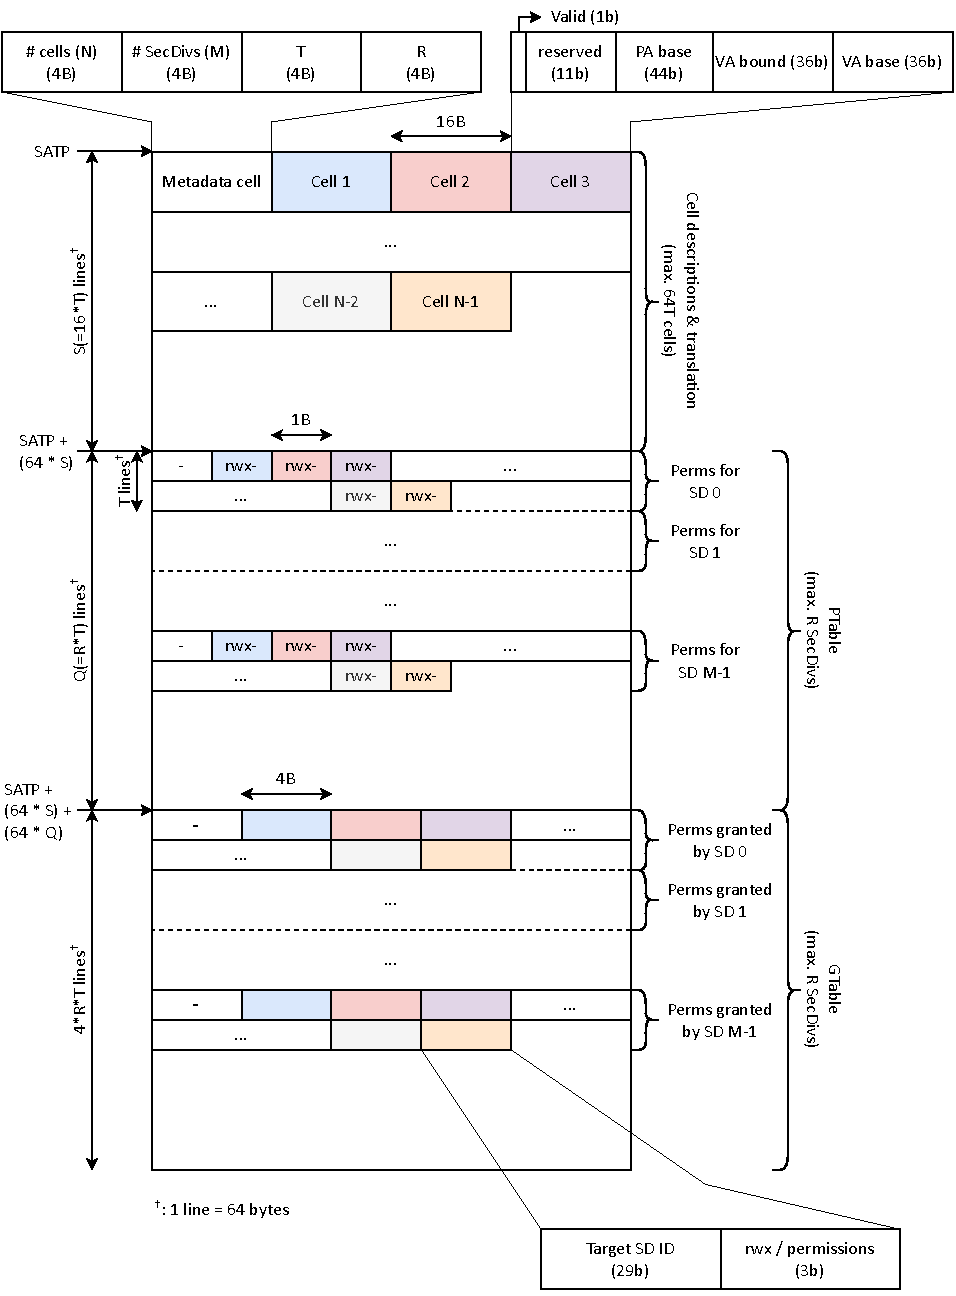
\includegraphics[height=0.95\textheight]{media/seccells/ptable_layout.pdf}
  \caption{Layout of the unified \ptable-\gtable.}
  \label{fig:ptable_layout}
  %\Description[<short description>]{<long description>}
\end{figure*}
\end{comment}

\section{Justification for \autoref{tab:req_comparison}}
\label{app:justification_table1}

\paragraph{Obj. \req{1a}}
MPK, ERIM and Donky do not check permissions for instruction fetches, 
simplifying code injection.
Under our threat model, an attacker can inject \Code{wrpkru} instructions 
to corrupt permissions.

\paragraph{Obj. \req{1b}}
Through code injection, call gates in MPK and ERIM can be bypassed.

\paragraph{Obj. \req{1c}}
CODOM requires migrating threads without context isolation.
MPK, ERIM and Donky rely on call gates if context isolation is desired.
However, MPK and ERIM cannot enforce call gates under our threat model.
Donky gives no mechanism for a compartment to restore its state without
trusting general-purpose registers. 
Further, Donky cannot adopt a \seccells-like software approach because a 
compartment has no way to identify itself.

\paragraph{Obj. \req{1d}}
CHERI allows one compartment to unilaterally send a capability to another compartment, 
unchecked by the TCB and unacknowledged by the receiver.

\paragraph{Obj. \req{1e}}
No mechanism except XPC considers the challenge of exclusive access.

\paragraph{Obj. \req{1f}}
A compartment in MPK and ERIM cannot check the value of the \Code{pkru}
register for another compartment, hindering audits.
Cross-core \Code{pkru} reads are not possible.
CHERI requires an expensive full memory scan for capabilities to perform
an audit.

\paragraph{Obj. \req{2a}}
Page-table based translation and permission checking encounter TLB-reach
limits leading to multi-cycle common case access verification for many
widely-used programs including \Code{memcached}. The mechanisms relying on
such page tables for either translation or permission checking fail this
requirement.

\paragraph{Obj. \req{2b}}
Supervisor-mediated cross-compartment calls in UNIX-like OSs,
Mondrian, lwC and CHERI require 100s or 1000s of cycles to complete.

\paragraph{Obj. \req{2c}}
Supervisor-mediated permission transfers are slow (UNIX, MMP, lwC).
MMP proposes the use of redundant mappings with different permissions
to implement a form of zero-copy transfer which is not generic.
CODOM does not really support permission transfers.
XPC restricts permission transfer to a single relay segment.

\paragraph{Obj. \req{3a}}
CODOM identifies the executing compartment by the instruction pointer, 
limiting the flexibility to share code/data regions between compartments.

\paragraph{Obj. \req{3b}}
UNIX, MMP, lwC, XPC and CHERI cannot eliminate context switching when a
permissive policy allows migrating threading between compartments.

\section{Existing mechanisms with \seccells}
\label{app:integrate_exist}
Many existing performance or security mechanisms can be integrated with
\seccells, either unmodified or with modifications described in this section.

\paragraph{Physical Memory Protections}
\seccells enforces permissions on the virtual address space, and is therefore
trivially compatible with physical memory protection schemes 
including RISC-V's Physical Memory Protection (PMP) mechanism, 
processor reserved memory for Intel's SGX
and vendor-specific protections like Qualcomm's XPU~\cite{qualcomm_ac}.
These mechanisms will apply to the physical address output by 
\seccells' MMU after \ptable access control checks.

\paragraph{Pointer authentication and capabilities}
ARM's pointer authentication code (PAC) feature and CHERI's capabilities
improve memory safety by protecting pointers from illegal 
modifications (overwriting when stored in memory and out-of-bound
increment respectively). Both mechanisms are orthogonal to,
and can integrate with \seccells, which checks accessess against \ptable
permissions when the 
pointers protected by these mechanisms are finally dereferenced, providing
another layer of protection against attacks like PACMAN~\cite{pacmanRavichandranNLY22}.

\paragraph{Hardware and Software Control Flow Integrity}
Hardware (e.g., Intel CET) and software (e.g., LLVM-CFI) control-flow
protections can integrate with \seccells, 
improving intra-compartment control-flow protection to
complement \seccells' inter-compartment call gates (\sdentry).
CET can continue to check indirect call targets for \Code{endbr} instructions. 
LLVM's and other fine-grained CFI pointer checks are implemented in software, 
orthogonal to hardware control flow checks.


\paragraph{Page-based mechanisms}
By itself, \seccells restricts popular mechanisms (e.g., guard pages, swapping)
operating on pages and page tables since translations and protections are 
tracked at \cell granularity.
However, \seccells can be integrated with upcoming intermediate address-space 
systems like Midgard re-enabling programmers to implement these crucial 
features.
Midgard couples \seccells-like range-based translation at the core with
a second level of page-granularity translations at the backside of the 
last-level cache.
Guard pages and swapping can both be implemented by unmapping the requisite pages 
in the backside translation.


\section{Speculative Side-Channel Attacks}
\label{app:sidechannel}

We consider the threat of speculative side-channel attacks like 
Spectre~\cite{KocherHFGGHHLM019}
in \seccells' design, despite omitting such attacks from our attacker model.
\seccells{} introduces additional mechanisms for changing an executing
thread's permissions, through userspace compartment switching and
permission transfers.
Fault-based attacks like Meltdown~\cite{lipp18sec} must be prevented in
implementations by preventing faulting loads from accessing memory or
forwarding their data to subsequent instructions~\cite{WeisseNLWK19}.

\seccells specifies that userspace instructions are serializing, 
precluding speculative permission changes.
An attacker cannot, for example, speculatively switch to a victim
\secdiv using an \sdswitch following a long-latency branch and read 
the victim's private data using the victim's permissions.
\seccells' permission transfer instructions are atomic, preventing visibility 
or exploitation of any intermediate permission state.
An attacker \secdiv cannot, for example, drop permissions for a \cell
using \scprot while transferring the same permissions using \sctfer in parallel.
Our firmware (and future microcode) implementation use load-linked 
store-conditional atomic operations commonly available across architectures
to ensure atomicity.
\seccells allows the pipeline to speculate as usual within a compartment's 
execution, and speculative accesses are also subject to access control 
by the MMU and cannot illegally access any \cell.
Access control, therefore, also limits the leakage potential of existing
Spectre gadgets.
Whereas a Spectre gadget on a traditional processor can address and
access any user memory in the process' address space, the same Spectre
gadget can only access memory within the compartment's \cell{}s.
\seccells also limits the code (speculatively) executable within a compartment,
further restricting the availability of Spectre gadgets.

\section{\seccells Implementation Trade-Offs}
\label{app:impl_options}

\seccells permits a range of implementations scaling from simple 
microcontrollers with firmware emulation for added userspace
instructions to server grade processors with microcode or hardware 
implementations. In this section, we describe the trade-offs and 
justify our implementation in \autoref{sec:impl}.

\paragraph{Firmware}
On the simplest side of the spectrum, instructions can be emulated
by firmware using trap-and-emulate.
Firmware is programmable code which runs in a privileged execution mode 
and uses native ISA instructions.
\seccells' instructions will trap into firmware, and be dispatched to 
the emulation code.
Firmware implementations are cheap, requiring no additional hardware, but 
slower than alternate implementations.
For the simple RISC-V RocketChip microcontroller, we choose 
firmware emulation for permission transfer instructions.
Note that the firmware can also forward traps to be emulated by
either the supervisor or even a privileged userspace library.
However, the additional security risk of emulation by less trusted
software risk and the overhead of forwarding traps makes such
implementations less attractive.

\paragraph{Hardware}
Alternatively, instructions can be implemented in hardware with 
finite-state machine circuits.
While this design option implies better performance,
designing complex hardware comes with silicon and power costs and
substantial complexity.
Hardware bug fixes incur the significant cost of the tape-out process.
Server and desktop processors generally include beefy cores with
large silicon area, where hardware implementations may match the
processor's targeted performance.
We implement the crucial \sdswitch instruction in hardware
to reap the performance advantage,
and because of the simplicity of its design.

\paragraph{Microcode}
A third option, microcode, is programmable code provided by the 
processor manufacturer, built from low level operations including ones 
not available through the ISA interface.
When a instruction implemented in microcode is encountered, a microcode
sequencer fetches microcode from an on-chip RAM and executes them in the
pipeline.
Microcode eliminates the cost of trapping and dispatch encountered in 
firmware emulation ($77\%$ of the latency of emulating \scprot),
and can also leverage hardware-specific optimizations.
Microcode is popular for implementing complicated instructions
with high performance like SGX's \Code{EENTER}/\Code{EEXIT} instructions.
Microcode also has the advantage of being programmable, and have been
leveraged to fix processor errata and bugs.
While the simple RocketChip lacks a microcode sequencer, 
we envision microcode to be ideal for implementing \seccells'
permission transfer instructions for high-performance processors.
\end{appendices}

%-------------------------------------------------------------------------------
\backmatter

\bibliographystyle{IEEEtran}
\phantomsection
\addcontentsline{toc}{chapter}{Bibliography}
\bibliography{thesis}


\end{document}
% End of Thesis CORE
%%%%%%%%%%%%%%%%%%%%%%%%%%%%%%%%%%%%%%%%%%%%%%%%%%%%%%%%%%%%%%%%%%%%%